%  LaTeX support: latex@mdpi.com 
%  For support, please attach all files needed for compiling as well as the log file, and specify your operating system, LaTeX version, and LaTeX editor.

%=================================================================
\documentclass[mathematics,article,accept,pdftex,moreauthors]{Definitions/mdpi} 
%\documentclass[preprints,article,submit,pdftex,moreauthors]{Definitions/mdpi} 
% For posting an early version of this manuscript as a preprint, you may use "preprints" as the journal. Changing "submit" to "accept" before posting will remove line numbers.

% Below journals will use APA reference format:
% admsci, behavsci, businesses, econometrics, economies, education, ejihpe, famsci, games, humans, ijcs, ijfs, journalmedia, jrfm, languages, psycholint, publications, tourismhosp, youth

% Below journals will use Chicago reference format:
% arts, genealogy, histories, humanities, jintelligence, laws, literature, religions, risks, socsci

%-
% Class Options:
%-
%-
% journal
%-
% Choose between the following MDPI journals:
% accountaudit, acoustics, actuators, addictions, adhesives, admsci, adolescents, aerobiology, aerospace, agriculture, agriengineering, agrochemicals, agronomy, ai, air, algorithms, allergies, alloys, amh, analytica, analytics, anatomia, anesthres, animals, antibiotics, antibodies, antioxidants, applbiosci, appliedchem, appliedmath, appliedphys, applmech, applmicrobiol, applnano, applsci, aquacj, architecture, arm, arthropoda, arts, asc, asi, astronomy, atmosphere, atoms, audiolres, automation, axioms, bacteria, batteries, bdcc, behavsci, beverages, biochem, bioengineering, biologics, biology, biomass, biomechanics, biomed, biomedicines, biomedinformatics, biomimetics, biomolecules, biophysica, biosensors, biosphere, biotech, birds, blockchains, bloods, blsf, brainsci, breath, buildings, businesses, cancers, carbon, cardiogenetics, catalysts, cells, ceramics, challenges, chemengineering, chemistry, chemosensors, chemproc, children, chips, cimb, civileng, cleantechnol, climate, clinbioenerg, clinpract, clockssleep, cmd, cmtr, coasts, coatings, colloids, colorants, commodities, complications, compounds, computation, computers, condensedmatter, conservation, constrmater, cosmetics, covid, crops, cryo, cryptography, crystals, csmf, ctn, curroncol, cyber, dairy, data, ddc, dentistry, dermato, dermatopathology, designs, devices, diabetology, diagnostics, dietetics, digital, disabilities, diseases, diversity, dna, drones, dynamics, earth, ebj, ecm, ecologies, econometrics, economies, education, eesp, ejihpe, electricity, electrochem, electronicmat, electronics, encyclopedia, endocrines, energies, eng, engproc, ent, entomology, entropy, environments, epidemiologia, epigenomes, esa, est, famsci, fermentation, fibers, fintech, fire, fishes, fluids, foods, forecasting, forensicsci, forests, fossstud, foundations, fractalfract, fuels, future, futureinternet, futureparasites, futurepharmacol, futurephys, futuretransp, galaxies, games, gases, gastroent, gastrointestdisord, gastronomy, gels, genealogy, genes, geographies, geohazards, geomatics, geometry, geosciences, geotechnics, geriatrics, glacies, grasses, greenhealth, gucdd, hardware, hazardousmatters, healthcare, hearts, hemato, hematolrep, heritage, higheredu, highthroughput, histories, horticulturae, hospitals, humanities, humans, hydrobiology, hydrogen, hydrology, hygiene, idr, iic, ijerph, ijfs, ijgi, ijmd, ijms, ijns, ijpb, ijt, ijtm, ijtpp, ime, immuno, informatics, information, infrastructures, inorganics, insects, instruments, inventions, iot, j, jal, jcdd, jcm, jcp, jcs, jcto, jdad, jdb, jeta, jfb, jfmk, jimaging, jintelligence, jlpea, jmahp, jmmp, jmms, jmp, jmse, jne, jnt, jof, joitmc, joma, jop, jor, journalmedia, jox, jpbi, jpm, jrfm, jsan, jtaer, jvd, jzbg, kidney, kidneydial, kinasesphosphatases, knowledge, labmed, laboratories, land, languages, laws, life, lights, limnolrev, lipidology, liquids, literature, livers, logics, logistics, lubricants, lymphatics, machines, macromol, magnetism, magnetochemistry, make, marinedrugs, materials, materproc, mathematics, mca, measurements, medicina, medicines, medsci, membranes, merits, metabolites, metals, meteorology, methane, metrics, metrology, micro, microarrays, microbiolres, microelectronics, micromachines, microorganisms, microplastics, microwave, minerals, mining, mmphys, modelling, molbank, molecules, mps, msf, mti, multimedia, muscles, nanoenergyadv, nanomanufacturing, nanomaterials, ncrna, ndt, network, neuroglia, neurolint, neurosci, nitrogen, notspecified, nursrep, nutraceuticals, nutrients, obesities, oceans, ohbm, onco, oncopathology, optics, oral, organics, organoids, osteology, oxygen, parasites, parasitologia, particles, pathogens, pathophysiology, pediatrrep, pets, pharmaceuticals, pharmaceutics, pharmacoepidemiology, pharmacy, philosophies, photochem, photonics, phycology, physchem, physics, physiologia, plants, plasma, platforms, pollutants, polymers, polysaccharides, populations, poultry, powders, preprints, proceedings, processes, prosthesis, proteomes, psf, psych, psychiatryint, psychoactives, psycholint, publications, purification, quantumrep, quaternary, qubs, radiation, reactions, realestate, receptors, recycling, regeneration, religions, remotesensing, reports, reprodmed, resources, rheumato, risks, robotics, rsee, ruminants, safety, sci, scipharm, sclerosis, seeds, sensors, separations, sexes, signals, sinusitis, siuj, skins, smartcities, sna, societies, socsci, software, soilsystems, solar, solids, spectroscj, sports, standards, stats, std, stresses, surfaces, surgeries, suschem, sustainability, symmetry, synbio, systems, tae, targets, taxonomy, technologies, telecom, test, textiles, thalassrep, therapeutics, thermo, timespace, tomography, tourismhosp, toxics, toxins, transplantology, transportation, traumacare, traumas, tropicalmed, universe, urbansci, uro, vaccines, vehicles, venereology, vetsci, vibration, virtualworlds, viruses, vision, waste, water, wem, wevj, wild, wind, women, world, youth, zoonoticdis

%-
% article
%-
% The default type of manuscript is "article", but can be replaced by: 
% abstract, addendum, article, benchmark, book, bookreview, briefcommunication, briefreport, casereport, changes, clinicopathologicalchallenge, comment, commentary, communication, conceptpaper, conferenceproceedings, correction, conferencereport, creative, datadescriptor, discussion, entry, expressionofconcern, extendedabstract, editorial, essay, erratum, fieldguide, hypothesis, interestingimages, letter, meetingreport, monograph, newbookreceived, obituary, opinion, proceedingpaper, projectreport, reply, retraction, review, perspective, protocol, shortnote, studyprotocol, supfile, systematicreview, technicalnote, viewpoint, guidelines, registeredreport, tutorial,  giantsinurology, urologyaroundtheworld
% supfile = supplementary materials

%-
% submit
%-
% The class option "submit" will be changed to "accept" by the Editorial Office when the paper is accepted. This will only make changes to the frontpage (e.g., the logo of the journal will get visible), the headings, and the copyright information. Also, line numbering will be removed. Journal info and pagination for accepted papers will also be assigned by the Editorial Office.

%-
% moreauthors
%-
% If there is only one author the class option oneauthor should be used. Otherwise use the class option moreauthors.

%-
% pdftex
%-
% The option pdftex is for use with pdfLaTeX. Remove "pdftex" for (1) compiling with LaTeX & dvi2pdf (if eps figures are used) or for (2) compiling with XeLaTeX.

%=================================================================
% MDPI internal commands - do not modify
\firstpage{1} 
\makeatletter 
\setcounter{page}{\@firstpage} 
\makeatother
\pubvolume{1}
\issuenum{1}
\articlenumber{0}
\pubyear{2026}
\copyrightyear{2026}
\externaleditor{Antanas Cenys} % More than 1 editor, please add `` and '' before the last editor name
\datereceived{11 March 2026} 
\daterevised{17 April 2026} % Comment out if no revised date
\dateaccepted{28 April 2026} 
\datepublished{ } 
%\datecorrected{} % For corrected papers: "Corrected: XXX" date in the original paper.
%\dateretracted{} % For retracted papers: "Retracted: XXX" date in the original paper.
\hreflink{https://doi.org/} % If needed use \linebreak
%\doinum{}
%\pdfoutput=1 % Uncommented for upload to arXiv.org
%\CorrStatement{yes}  % For updates
%\longauthorlist{yes} % For many authors that exceed the left citation part
%\IsAssociation{yes} % For association journals

%=================================================================
% Add packages and commands here. The following packages are loaded in our class file: fontenc, inputenc, calc, indentfirst, fancyhdr, graphicx, epstopdf, lastpage, ifthen, float, amsmath, amssymb, lineno, setspace, enumitem, mathpazo, booktabs, titlesec, etoolbox, tabto, xcolor, colortbl, soul, multirow, microtype, tikz, totcount, changepage, attrib, upgreek, array, tabularx, pbox, ragged2e, tocloft, marginnote, marginfix, enotez, amsthm, natbib, hyperref, cleveref, scrextend, url, geometry, newfloat, caption, draftwatermark, seqsplit
% cleveref: load \crefname definitions after \begin{document}
\usepackage{makecell}
\usepackage{tikz}
\usetikzlibrary{shapes.geometric,shadows,arrows.meta,positioning}

% Define styles
\tikzstyle{process} = [
  rectangle, 
  minimum width=3cm, 
  minimum height=1cm, 
  text centered, 
  draw=black, 
  fill=gray!30,
  rounded corners,
  align=center
]
\tikzstyle{decision} = [
  diamond, 
  minimum width=3cm, 
  minimum height=1cm, 
  text centered, 
  draw=black, 
  fill=gray!30,
  align=center
]
\tikzstyle{arrow} = [
  thick, 
  ->, 
  >=Stealth
]

\usepackage{svg}

\usepackage{xcolor}

% ===== CHANGES DISPLAY TOGGLE =====
% \finaloutputfalse  -> DRAFT: show all markup in colour
% \finaloutputtrue   -> FINAL: clean output, no markup (avoids etb@tempa clash)
%\newif\iffinaloutput
%\finaloutputfalse   % <- change to \finaloutputtrue for clean output
%
%\iffinaloutput
%  % Final mode: accept all additions, drop all deletions silently
%  \newcommand{\add}[1]{#1}
%  \newcommand{\remove}[1]{}
%  \newcommand{\change}[2]{#2}
%  \newcommand{\note}[2][]{}
%\else
%  % Draft mode: show tracked changes with coloured markup
%  \usepackage{changes}
%  \newcommand{\add}[1]{\added{#1}}
%  \newcommand{\remove}[1]{\deleted{#1}}
%  \newcommand{\change}[2]{\replaced{#2}{#1}}
%  \newcommand{\note}[2][]{}
%\fi
%
\definecolor{insecure}{RGB}{255,220,220}
\definecolor{humanscale}{RGB}{255,245,200}
\definecolor{supersecure}{RGB}{220,245,220}

%=================================================================
% Please use the following mathematics environments: Theorem, Lemma, Corollary, Proposition, Characterization, Property, Problem, Example, ExamplesandDefinitions, Hypothesis, Remark, Definition, Notation, Assumption
%% For proofs, please use the proof environment (the amsthm package is loaded by the MDPI class).

%=================================================================
% Full title of the paper (Capitalized)
\Title{GeoVault: Leveraging Human Spatial Memory for Secure Cryptographic Key Management}

% MDPI internal command: Title for citation in the left column
%\TitleCitation{Title}

% Author Orchid ID: enter ID or remove command
\newcommand{\orcidauthorA}{0000-0003-1679-5306} % Add \orcidA{} behind the author's name
%\newcommand{\orcidauthorB}{0000-0000-0000-000X} % Add \orcidB{} behind the author's name

% Authors, for the paper (add full first names)
\Author{Marko Corn\orcidA{} * and Primož Podržaj}
 
%\longauthorlist{yes}

% MDPI internal command: Authors, for metadata in PDF
\AuthorNames{Marko Corn and Primož Podržaj}



% Affiliations / Addresses (Add [1] after \address if there is only one affiliation.)
\address[1]{Faculty of Mechanical Engineering, University of Ljubljana, 1000 Ljubljana, Slovenia; primoz.podrzaj@fs.uni-lj.si}


% Contact information of the corresponding author
\corres{\hangafter=1 \hangindent=1.05em \hspace{-0.82em}Correspondence: marko.corn@fs.uni-lj.si}


% Current address and/or shared authorship
%\firstnote{Current address: Affiliation.}  % Placeholder removed; add real current address if applicable.
%\firstnote{\hangafter=1 \hangindent=1.05em \hspace{-0.82em}These authors contributed equally to this work.}
% The commands \thirdnote{} till \eighthnote{} are available for further notes

%\simplesumm{} % Simple summary

%\conference{} % An extended version of a conference paper

% Abstract (Do not insert blank lines, i.e. \\) 
\abstract{
%\remove{Human-centered cryptographic key management is constrained by a persistent tension between security and usability. While modern cryptographic primitives offer strong theoretical guarantees, practical failures often arise from the difficulty users face in generating, memorizing, and securely storing high-entropy secrets. Existing mnemonic approaches suffer from severe entropy collapse due to predictable human choice, while machine-generated mnemonics such as BIP-39 impose significant cognitive burden. This paper introduces \textit{GeoVault}, a spatially anchored key derivation framework that leverages human spatial memory as a cryptographic input. GeoVault derives keys from user-selected geographic locations, encoded deterministically and hardened using memory-hard key derivation functions. We develop a formal entropy model that captures semantic and clustering biases in human location choice and distinguishes nominal from effective spatial entropy under attacker-prioritized dictionaries. Through information-theoretic analysis and CPU-GPU benchmarking, we show that spatially anchored secrets provide a substantially higher effective entropy floor than human-chosen passwords under realistic attacker models. We introduce the \textit{GPU throughput advantage} $\eta(m) = R_\text{GPU}(m) \cdot T_\text{CPU}(m)$ as a metric for the defender-attacker asymmetry: at the practical reference tier of $m = 1{,}024$\,MiB, $\eta \approx 66$, meaning the attacker can test 66 candidates per one defender key derivation. KDF chaining depth $k$ does not improve $\eta$, as it scales both sides equally; only increasing $m$ toward GPU VRAM saturation drives $\eta$ downward. Crucially, the exponential search-space expansion from spatial multi-point selection ($n \geq 3$) provides security margins orders of magnitude larger than $\eta$, absorbing the residual throughput advantage entirely. Under a demographically targeted attacker prior (anchor entropy $\approx 27.4$\,bits), selecting $n \geq 3$ spatial points is necessary and sufficient to maintain cryptographic-strength resistance; single-point configurations remain in the Insecure zone regardless of computational hardening.}
{Practical failures of cryptographic key management rarely stem from weak algorithms: they arise from the difficulty users face in memorizing and reliably recalling high-entropy secrets. Password-based and brainwallet approaches collapse under selection bias, while machine-generated mnemonics such as BIP-39 impose a significant memory burden. This paper introduces \textit{GeoVault}, a key derivation framework that uses remembered geographic locations as the cryptographic input. Keys are derived from a small set of user-selected map points, encoded deterministically using a geospatial scheme and hardened with the Argon2id memory-hard function. We develop a formal entropy model that distinguishes nominal from effective spatial entropy under attacker-prioritized geographic dictionaries and quantifies the additional reduction caused by demographic selection bias. Through information-theoretic analysis and CPU-GPU benchmarking, we show that spatial secrets carry a substantially higher effective entropy floor than human-chosen passwords, and that Argon2id creates a strong asymmetry between legitimate users and offline adversaries: at a memory cost of 1\,GiB, an attacker using a high-end GPU can test approximately 66 candidate secrets per one defender key derivation. This residual throughput advantage is, however, overwhelmed by the exponential growth of the search space when multiple locations are selected. Selecting $n \geq 3$ geographic points is necessary and sufficient to achieve cryptographic-strength brute-force resistance under the global attacker prior across all evaluated Argon2id configurations. Against a demographically targeted attacker with city-level knowledge of the user, $n=3$ maintains Human-Scale Secure resistance; $n=4$ with a chaining depth of $k=6$ restores the Super Secure zone at an $\approx$8\,s user-side wait. Single-point configurations remain insecure regardless of memory cost hardening.}}


% Keywords
\keyword{cryptographic key management; spatial memory; mnemonic security; entropy modeling; memory-hard key derivation; Argon2; brainwallet security; human-centered cryptography}


% The fields PACS, MSC, and JEL may be left empty or commented out if not applicable
%\PACS{J0101}
\MSC{94A17; 94A60; 68P25}
%\JEL{}

%%%%%%%%%%%%%%%%%%%%%%%%%%%%%%%%%%%%%%%%%%
% Only for the journal Diversity
%\LSID{\url{http://}}

%%%%%%%%%%%%%%%%%%%%%%%%%%%%%%%%%%%%%%%%%%
% Only for the journal Applied Sciences
%\featuredapplication{Authors are encouraged to provide a concise description of the specific application or a potential application of the work. This section is not mandatory.}
%%%%%%%%%%%%%%%%%%%%%%%%%%%%%%%%%%%%%%%%%%

%%%%%%%%%%%%%%%%%%%%%%%%%%%%%%%%%%%%%%%%%%
% Only for the journal Data
%\dataset{DOI number or link to the deposited data set if the data set is published separately. If the data set shall be published as a supplement to this paper, this field will be filled by the journal editors. In this case, please submit the data set as a supplement.}
%\datasetlicense{License under which the data set is made available (CC0, CC-BY, CC-BY-SA, CC-BY-NC, etc.)}

%%%%%%%%%%%%%%%%%%%%%%%%%%%%%%%%%%%%%%%%%%
% Only for the journal Toxins
%\keycontribution{The breakthroughs or highlights of the manuscript. Authors can write one or two sentences to describe the most important part of the paper.}

%%%%%%%%%%%%%%%%%%%%%%%%%%%%%%%%%%%%%%%%%%
% Only for the journal Encyclopedia
%\encyclopediadef{For entry manuscripts only: please provide a brief overview of the entry title instead of an abstract.}

%%%%%%%%%%%%%%%%%%%%%%%%%%%%%%%%%%%%%%%%%%
% Only for the journal Advances in Respiratory Medicine, Smart Cities and Sensors
%\addhighlights{yes}
%\renewcommand{\addhighlights}{%
%
%\noindent This is an obligatory section in “Advances in Respiratory Medicine'' and ``Smart Cities”, whose goal is to increase the discoverability and readability of the article via search engines and other scholars. Highlights should not be a copy of the abstract, but a simple text allowing the reader to quickly and simplified find out what the article is about and what can be cited from it. Each of these parts should be devoted up to 2~bullet points.\vspace{3pt}\\
%\textbf{What are the main findings?}
% \begin{itemize}[labelsep=2.5mm,topsep=-3pt]
% \item First bullet.
% \item Second bullet.
% \end{itemize}\vspace{3pt}
%\textbf{What is the implication of the main finding?}
% \begin{itemize}[labelsep=2.5mm,topsep=-3pt]
% \item First bullet.
% \item Second bullet.
% \end{itemize}
%}

%%%%%%%%%%%%%%%%%%%%%%%%%%%%%%%%%%%%%%%%%%
\begin{document}

%%%%%%%%%%%%%%%%%%%%%%%%%%%%%%%%%%%%%%%%%%
% \setcounter{section}{} %% Remove this when starting to work on the template.
% \section{
% How to Use this Template}

% The template details the sections that can be used in a manuscript. Note that the order and names of article sections may differ from the requirements of the journal (e.g., the positioning of the Materials and Methods section). Please check the instructions on the authors' page of the journal to verify the correct order and names. For any questions, please contact the editorial office of the journal or support@mdpi.com. For LaTeX-related questions please contact latex@mdpi.com.

%\endnote{This is an endnote.} % To use endnotes, please un-comment \printendnotes below (before References). Only journal Laws uses \footnote.

% The order of the section titles is different for some journals. Please refer to the "Instructions for Authors” on the journal homepage.

\section{Introduction}

%\remove{Secure cryptographic key management remains one of the most persistent usability challenges in modern security systems. While cryptographic primitives themselves have achieved a high degree of mathematical maturity, real-world security failures are frequently caused not by algorithmic weaknesses, but by the difficulty humans face in generating, storing, and reliably recalling high-entropy secrets. This mismatch between human cognitive capabilities and cryptographic requirements has motivated a wide range of mnemonic key storage approaches, including password-based systems, brainwallets, and standardized mnemonic phrases such as BIP-39.}
{Cryptographic algorithms rarely fail in isolation; real-world security breaches are far more often caused by the difficulty humans face in generating, storing, and reliably recalling high-entropy secrets~\cite{Adams1999}. This constraint has driven two decades of research into mnemonic key storage: password managers, brainwallets, and standardized phrase lists such as BIP-39 each represent a different point in the trade-off space between entropy \mbox{and memorability.}}

Brainwallets and passphrase-derived keys attempt to eliminate the need for external storage by relying entirely on human memory. However, extensive empirical research has shown that such approaches fail under realistic offline attacker models due to severe entropy collapse caused by predictable human choice~\cite{Bonneau2012,Vasek2017}. Large-scale studies of real-world password datasets demonstrate that users consistently select secrets with strong linguistic and cultural bias, resulting in effective entropy levels far below theoretical estimates~\cite{Bonneau2012,Kuo2006}. Analyses of funded brainwallets further confirm that passphrase-derived keys are often compromised shortly after use, sometimes within minutes~\cite{Vasek2017,Yang2016}. Even mnemonic-friendly strategies fail to provide durable protection once human selection bias is taken into account.

In contrast, machine-generated mnemonic schemes such as BIP-39 offer strong cryptographic guarantees by selecting words uniformly from a fixed dictionary, yielding well-defined entropy budgets. A standard 12-word BIP-39 mnemonic provides 128 bits of nominal entropy, making exhaustive brute-force attacks computationally infeasible under conventional assumptions. However, these schemes impose a significant cognitive burden on users, who must reliably store or back up the mnemonic phrase. In practice, this often leads to insecure storage practices or irreversible loss of access, effectively shifting the problem from entropy generation to key retention and recovery.

%\remove{A key limitation shared by most existing mnemonic systems is their dependence on linguistic or abstract symbolic memory, which is known to be fragile and error-prone over long time horizons~\cite{Pals2018,Akaygun2014}. In contrast, decades of research in cognitive psychology and neuroscience have established that humans possess a robust capacity for spatial memory. Spatial representations are encoded, organized, and retrieved using dedicated cognitive mechanisms centered around landmarks and reference frames, and are retained accurately even after long periods without rehearsal~\cite{Montello1998,McNamara2003,McNamara2012}. Neurobiological evidence further supports this distinction: the hippocampus plays a central role in both spatial navigation and long-term memory formation, suggesting a deep functional link between spatial awareness and memory encoding~\cite{McNaughton1991}.}
{Despite their differences, password-based and brainwallet approaches share a common dependency: linguistic or abstract symbolic memory, a form of recall that degrades measurably over months and years~\cite{Pals2018,Akaygun2014}. Spatial memory follows a strikingly different retention profile. Layouts of familiar places, routes, and personal landmarks are encoded through hippocampal circuits that govern long-term spatial navigation and are retained with high fidelity even after long intervals without rehearsal~\cite{Montello1998,McNamara2003,McNamara2012,McNaughton1991}. The difference is not incidental: it reflects distinct cognitive mechanisms, with verbal recall rapidly susceptible to interference and spatial recall comparatively stable.}

%\remove{These findings have motivated prior work exploring graphical and spatially inspired authentication mechanisms~\cite{Tari2006,Golla2017}. While such systems demonstrate improved memorability compared to textual passwords, they typically suffer from limited entropy, susceptibility to observation attacks, or strong user bias toward predictable choices. As a result, spatial memory has not yet been systematically integrated into cryptographic key derivation frameworks with explicit entropy modeling and hardware-aware offline threat assumptions.}
{Prior authentication research has drawn on related intuitions, exploring graphical and map-based schemes~\cite{Tari2006,Golla2017,Sun2012,Thorpe2013}. User studies confirm improved recall, but the security question has been handled qualitatively: none of these systems couples spatial selection to a formal entropy model, quantifies the reduction caused by demographic selection bias, or evaluates the resulting work factor against a GPU-class offline adversary with access to attacker-prioritized spatial dictionaries.}

In parallel, advances in cryptographic key derivation functions have made it possible to impose strong, hardware-enforced asymmetries between legitimate users and offline adversaries. Memory-hard functions such as Argon2 were explicitly designed to resist massively parallel GPU and ASIC attacks by binding performance to memory bandwidth and capacity rather than raw compute throughput~\cite{7467361,Wetzels2016}. Empirical studies have shown that such functions significantly reduce attacker advantage and allow defenders to trade modest increases in computation time for large increases in brute-force resistance~\cite{Choe2019}.

This paper introduces \textit{GeoVault}, a key management framework that combines these insights. GeoVault derives cryptographic keys from one or more user-selected spatial locations, encoded deterministically using geospatial encoding schemes and hardened through memory-hard key derivation. By anchoring secrets in spatial memory and amplifying their security through computational hardness, GeoVault aims to mitigate the security--usability limitations inherent in brainwallet-style systems under offline attack models.

%\remove{The contributions of this work are threefold:}
{The main contributions of this work are as follows:}
\begin{itemize}
\item We introduce a formal entropy model for spatially anchored secrets that distinguishes nominal spatial entropy from effective entropy under attacker-prioritized spatial dictionaries, capturing realistic semantic and clustering biases in human \mbox{location choice.}
\item We analyze and quantify the security limits of spatial memory under realistic human selection behavior, showing how clustering and semantic constraints reduce effective entropy and how multi-point spatial selection mitigates this effect.
\item We empirically evaluate the defender--attacker asymmetry induced by memory-hard key derivation using Argon2id, demonstrating that modest multi-point spatial selection combined with memory-hard derivation can achieve attacker-adjusted work factors that approach or, under certain configurations, exceed those of 12-word BIP-39 mnemonics, while single-point configurations provide meaningful offline resistance with reduced cognitive burden. We further characterize the effect of KDF chaining depth $k$ as an independent security axis, provide projected latency estimates across server, consumer laptop and smartphone hardware classes, and analyze GeoVault's security margins under quantum (Grover) and ASIC adversary models.
\end{itemize}



%\remove{The remainder of this paper is organized as follows. Section~2 reviews related work on brainwallets, mnemonic-based key storage, human memory limitations, spatial cognition, and geospatial encoding systems, highlighting the shortcomings of existing approaches and motivating the use of spatial memory as a cryptographic primitive. Section~3 introduces the theoretical foundations of the proposed approach, including formal entropy models for linguistic and spatial secrets, effective entropy under attacker-prioritized dictionaries, and the role of computational entropy boosting. Section~4 presents the design of the \textit{GeoVault} protocol, detailing the spatial selection process, geospatial encoding, entropy-boosting mechanisms, and the attacker-defender security evaluation methodology. Section~5 reports empirical results, including spatial entropy analysis, CPU-GPU asymmetry benchmarks, and the impact of memory-hard key derivation on attacker work factors under realistic hardware constraints. Section~6 discusses the implications of the results, examines limitations and threat model assumptions, and positions GeoVault within the broader landscape of human-centered key management. Finally, Section~7 concludes the paper and outlines directions for future research.}
{The paper is structured as follows. Section~\ref{sec2} reviews related work on brainwallets, mnemonic-based key storage, spatial cognition, and geospatial encoding. Section~\ref{sec3} develops the theoretical foundations, including formal entropy models, attacker-prioritized spatial dictionaries, and computational hardening. Section~\ref{sec4} presents the GeoVault protocol design. Section~\ref{sec5} reports the empirical benchmarks. Section~\ref{sec6} discusses implications and limitations. Section~\ref{sec7} concludes.}

\section{Related Work\label{sec2}}

\subsection{Brainwallets and Their Weaknesses\label{sec2.1}}

Brainwallets represent a class of deterministic cryptocurrency wallets in which private keys are derived directly from user-chosen passwords or passphrases. The underlying assumption is that users can reliably memorize sufficiently complex secrets, thereby eliminating the need for physical or digital storage of private keys~\cite{Das2019, Vasek2017}. In practice, however, extensive empirical research has demonstrated that this assumption is rarely satisfied, leading to severe security and usability limitations.

The core vulnerability of brainwallets stems from the predictable nature of human-chosen passwords and passphrases. Vasek et al.~\cite{Vasek2017} conducted a large-scale empirical analysis of funded brainwallets and showed that users overwhelmingly select easily guessable phrases, resulting in a dramatic reduction in effective entropy. Their findings revealed that the majority of brainwallets were compromised shortly after being funded, often within minutes, underscoring the practicality of offline dictionary attacks against passphrase-derived keys.

Earlier work by Kuo et al.~\cite{Kuo2006} identified similar weaknesses in mnemonic phrase-based passwords, demonstrating that users frequently rely on common phrases sourced from online material. Yang et al.~\cite{Yang2016} further confirmed that mnemonic-based password strategies, despite their perceived memorability benefits, produce secrets that remain highly vulnerable to statistical guessing attacks.

These vulnerabilities are compounded by fundamental cognitive limitations in human memory. Bonneau~\cite{Bonneau2012} demonstrated that, despite repeated efforts to promote stronger password practices, most users fail to achieve sufficient entropy in practice. Adams and Sasse~\cite{Adams1999, Sasse2001} explained this phenomenon from a usability perspective, arguing that increasing password complexity requirements directly conflicts with human memory constraints and predictably leads users toward insecure coping strategies.

Attempts to mitigate these weaknesses through user education have shown limited effectiveness. Kävrestad and Nohlberg~\cite{Kavrestad2020} found that context-based security training failed to produce meaningful improvements in real-world passphrase strength, highlighting the persistent tension between security requirements and human cognitive limitations.

Alternative authentication schemes that seek to exploit human visual memory have similarly encountered structural weaknesses. Tari et al.~\cite{Tari2006} and Golla et al.~\cite{Golla2017} investigated graphical and emoji-based password systems, identifying vulnerabilities such as susceptibility to shoulder-surfing and strong user bias toward predictable choices. While such approaches can improve memorability, they do not eliminate the fundamental problem of low effective entropy under targeted attack models.

To address the inherent weaknesses of brainwallets, alternative key management approaches have been proposed, including hierarchical deterministic (HD) wallets~\cite{DiLuzio2020, Gutoski2015} and hardware-based wallets, commonly referred to as cold wallets~\cite{Das2019,8726762}. HD wallets, standardized in BIP32, derive large key hierarchies from a single master seed, simplifying backup and recovery. However, Di Luzio et al.~\cite{DiLuzio2020} identified privilege escalation vulnerabilities in multi-user settings, while Gutoski and Stebila~\cite{Gutoski2015} demonstrated that partial key leakage can enable recovery of the master secret, exposing the entire wallet hierarchy.

Cold wallets mitigate network-based attacks by storing private keys offline, but they introduce distinct attack surfaces. Das et al.~\cite{Das2019} analyzed the hot/cold wallet paradigm and formalized conditions under which such systems remain secure. Nevertheless, Guri~\cite{8726762} experimentally demonstrated that air-gapped wallets can be compromised through physical side channels, including electromagnetic, acoustic, optical, and thermal leakage, challenging the assumption that hardware isolation alone provides absolute security.

In summary, brainwallets and mnemonic-based password schemes consistently suffer from two fundamental weaknesses: low effective entropy caused by predictable human-chosen secrets, and usability constraints rooted in cognitive limitations~\cite{Kuo2006, Vasek2017, Yang2016}. While HD wallets and cold wallets mitigate certain risks, they introduce additional complexity and new failure modes, such as master-key leakage~\cite{Gutoski2015, DiLuzio2020} or physical side-channel exfiltration~\cite{Das2019,8726762}. These limitations motivate the exploration of alternative approaches that align more closely with human cognitive strengths. In particular, leveraging spatial memory—an ability known for its robustness and long-term retention—offers a promising foundation for secure and user-friendly key management.

\subsection{Human Spatial Memory as a Cryptographic Asset}

%\remove{Human memory is notoriously unreliable when it comes to memorizing abstract information such as complex alphanumeric strings or passphrases~\cite{Pals2018, Akaygun2014}. However, decades of cognitive psychology research have shown that humans exhibit a disproportionately strong ability to encode, recall, and retain spatial information~\cite{montello1998new, McNamara2003}. This observation underpins the “method of loci,” an ancient memory technique that leverages imagined spatial environments to recall information by placing memories at physical locations within a mental map~\cite{Yates2013}.}

{Human memory is notoriously unreliable when it comes to memorizing abstract information such as complex alphanumeric strings or passphrases~\cite{Pals2018, Akaygun2014}. However, decades of cognitive psychology research have shown that humans exhibit a disproportionately strong ability to encode, recall, and retain spatial information~\cite{Montello1998, McNamara2003}. This observation underpins the ``method of loci,'' an ancient memory technique that leverages imagined spatial environments to recall information by placing memories at physical locations within a mental map~\cite{Yates2013}.}

Neurological evidence also supports the unique role of spatial memory in human cognition. The hippocampus, a brain structure critical for memory formation, is also central to spatial navigation~\cite{McNaughton1991}. The dual-use of this brain region suggests a strong evolutionary and functional link between spatial awareness and memory encoding. Studies in cognitive neuroscience confirm that people can recall spatial configurations with high accuracy even after long periods, particularly when these memories are grounded in visual or map-based stimuli~\cite{Konkle2010, Lukavsky2017}.

%\remove{More recently, spatial interfaces have been proposed in password systems and digital authentication~\cite{Bauer1993}. Although graphical passwords do not directly translate to geographic locations, their effectiveness demonstrates that spatially anchored memory cues are more durable than abstract password recall. In usability studies, users retained spatially-based authentication secrets for longer durations and with fewer errors compared to textual passphrases~\cite{Garden2002}.}

%\remove{These findings suggest that spatial memory may provide a superior foundation for cryptographic key storage and retrieval mechanisms. Unlike traditional brainwallets that rely on memorized strings, a system that anchors a seed derivation process to a spatial coordinate or map location would naturally exploit this cognitive strength. Such systems could offer both better security and usability, reducing the cognitive load while maintaining high entropy—especially when combined with computational functions that bind access to the correct location and effort.}

{Map-based authentication has been explored since at least \textit{PassMap}~\cite{Sun2012} and \textit{GeoPass}~\cite{Thorpe2013}, which showed that geographic secrets are retained for 3--5~weeks with fewer errors than alphanumeric passphrases. \textit{GeoPassNotes}~\cite{MacRae2016} further showed that personally meaningful landmarks improve recall by activating episodic memory cues.}

{Despite these advantages, prior work in map-based authentication has identified severe entropy collapse caused by predictable human selection. Users consistently exhibit strong semantic bias toward residential locations (home/work), major urban centers, and famous global landmarks~\cite{Sun2012, Thorpe2013, AlAmeen2014}. A comprehensive usability and security evaluation by Al-Ameen and Wright~\cite{AlAmeen2014} further quantified the degree to which user selection distributions concentrate around personally and culturally salient locations, confirming that an adversary with even limited contextual knowledge of the user can substantially reduce the effective search space below the nominal geographic entropy. These selection patterns reduce the effective search space in ways that purely geographic dictionaries do not capture. While these studies establish the memorability of spatial secrets, they have not yet been integrated into a cryptographic key derivation framework that explicitly mitigates selection bias through memory-hardening and hardware-aware offline threat modeling.}

{These findings suggest that spatial memory may provide a superior foundation for cryptographic key storage and retrieval mechanisms. Unlike traditional brainwallets that rely on memorized strings, a system that anchors a seed derivation process to a spatial coordinate or map location naturally exploits this cognitive strength. By combining the robustness of spatial recall with computational functions that bind access to the correct location and effort, it is possible to achieve both higher security and improved usability.}

\subsection{Geospatial Encoding Systems}

Geospatial encoding systems provide a structured way to represent geographic locations using codes or identifiers, facilitating applications such as navigation, logistics, and, in the context of this research, secure mnemonic storage based on spatial memory. These systems translate physical locations into a format that can be easily shared and processed, making them a critical component of the proposed \textit{GeoVault} protocol.

A widely recognized example is What3Words (w3w), which partitions the globe into 3~m $\times$
 3~m squares, each assigned a unique three-word identifier. This system excels in usability due to its intuitive word-based format, reducing errors compared to traditional coordinates, and supports multiple languages \cite{Jiang2018a}. However, its fixed resolution limits its flexibility for applications requiring finer granularity or three-dimensional encoding, such as indoor environments \cite{Lee2009}. Moreover, recent critiques highlight potential confusion between similar word triplets, posing risks in critical applications like emergency response or secure storage \cite{Arthur2023}. These limitations are particularly relevant to \textit{GeoVault}, where precise and unambiguous location encoding directly impacts mnemonic security.

Alternative systems include Geohash, Google's Open Location Code (OLC), and Google S2. Geohash employs a hierarchical grid with alphanumeric codes, offering variable precision but suffering from complexity and potential user confusion due to its base32 encoding \cite{Mai2022}. Open Location Code, designed for offline use, provides a more accessible alphanumeric approach, balancing usability and scalability \cite{Mai2022}. Google S2, optimized for spatial indexing, uses a cell-based structure that supports efficient querying and could enhance the protocol's computational efficiency \cite{Mai2022}. Each system presents distinct characteristics: Geohash and OLC prioritize flexibility, while S2 emphasizes performance in large-scale applications.

The choice of a geospatial encoding system for \textit{GeoVault} involves several trade-offs. Usability is critical for enabling users to recall and input locations accurately, favoring systems like What3Words \cite{Jiang2018a}. Granularity, or the size of the encoded area, affects the entropy of the system---a finer grid increases the number of possible locations, strengthening security against brute-force attacks. Encoding precision also influences the integration with computation-hard derivation functions like Argon2, as higher precision demands greater computational effort to protect the mnemonic seed. Additionally, reliability and accuracy are paramount, as geocoding errors can compromise the protocol's integrity. Studies reveal significant variability in geocoding accuracy across services and regions, necessitating robust validation frameworks \cite{Goldberg2013, Zandbergen2008a}.

In this research, geospatial encoding systems underpin the spatial anchoring of mnemonic seeds. While What3Words offers a compelling balance of usability and precision, its proprietary nature and potential for confusion \cite{Arthur2023} necessitate the exploration of open-source alternatives like Open Location Code for fully offline-resolvable implementations. Alternatives like Google S2 could improve scalability and precision, while custom schemes might better align with the protocol's security requirements \cite{Mai2022}. Furthermore, address extraction and matching techniques from web data, as explored in \cite{Efremova2018}, could enhance location selection, ensuring users choose memorable yet secure spatial anchors.

Ultimately, the selected system must integrate seamlessly with the protocol's threat model, resisting attacks such as map scanning or brute-forcing while maintaining user-friendliness. Future work will explore hybrid approaches, potentially combining What3Words' simplicity with S2's flexibility, and evaluate their performance in real-world mnemonic recovery scenarios.

\subsection{%\remove{Encryption Techniques for Burying Secrets} 
{Encryption Techniques for Hardening Secrets}}

%\remove{Secure storage of mnemonic seeds in the \textit{GeoVault} protocol relies on cryptographic techniques that impose significant computational barriers to unauthorized recovery while ensuring practical access for legitimate users. This section examines four mechanisms-memory-hard key derivation functions (KDFs), verifiable delay functions (VDFs), time-lock puzzles, and proofs of sequential work (PoSW)-that protect against brute-force attacks by leveraging memory, time, or sequential computation. Each technique is illustrated with a scientific example to demonstrate its role in securing spatially anchored mnemonic seeds.}

%\remove{Memory-hard KDFs, such as Argon2, transform inputs like spatial coordinates into cryptographic keys through processes that require substantial memory resources, thereby resisting optimization by hardware accelerators such as ASICs or GPUs~\cite{7467361,Wetzels2016}. For instance, Argon2d with parameters set to use 1 GB of memory and 10,000 iterations generates a 256-bit key from coordinates (e.g., 40.7128$^{\circ}$ N, 74.0060$^{\circ}$ W) by filling a 1 GB array with pseudorandom values and iteratively referencing it in a dependent pattern. An adversary with only 100 MB of memory must recompute missing blocks, increasing their runtime by a factor of 10,000 compared to a system with the full 1 GB. This memory-computation trade-off ensures that brute-forcing keys across multiple locations is resource-intensive, making large-scale attacks impractical. However, emerging compute-capable memory technologies, such as near-data processing, may reduce memory access costs, potentially weakening memory-hard functions like scrypt~\cite{Choe2019}, underscoring the need for adaptable KDFs.}

%\remove{Verifiable delay functions (VDFs) enforce a fixed number of sequential computational steps, with efficient verification of the result~\cite{Boneh2018,Wesolowski2019}. Consider a VDF based on repeated squaring: computing \( y = x^{2^t} \mod N \), where \( N \) is a 2048-bit RSA modulus, \( x \) is derived from the coordinates, and \( t = 10^6 \). On a 3 GHz CPU, each squaring takes approximately 1 microsecond, totaling 1 second for 1 million squarings. Even with 1,000 parallel CPUs, the sequential dependency ensures the computation still takes 1 second. Verification, however, is a single modular exponentiation, completed in milliseconds. This property is ideal for \textit{GeoVault}, as it imposes a mandatory delay on seed derivation, preventing rapid attacks while allowing quick validation. Recent VDF constructions achieve tight efficiency and reduce prover storage via incremental computation~\cite{Dottling2020,Dottling2019}, though their reliance on groups of unknown order may complicate implementation~\cite{Wesolowski2019}.}

%\remove{Time-lock puzzles encrypt data, such as a mnemonic seed, to be unlocked only after a predefined computational effort, typically through sequential operations~\cite{Mahmoody2011}. For example, a puzzle requiring \( t = 10^9 \) squarings modulo a 2048-bit \( N \) takes approximately 17 minutes on a high-end CPU performing 1 million squarings per second. The encryption might be structured as \( c = m + H(k)^{2^t} \mod N \), where \( m \) is the seed and \( H(k) \) is a hash of the coordinates. Decryption requires computing \( H(k)^{2^t} \) sequentially, with no parallelization benefit. This ensures that the seed remains inaccessible until the full computational effort is expended, mirroring the burial of a secret in \textit{GeoVault}. While constructions using repeated squaring or bilinear pairings offer provable security, they are vulnerable to advances in factoring or quantum attacks~\cite{Mahmoody2011,Cheon2008}. Non-interactive timed-release encryption schemes avoid server dependency but often rely on identity-based encryption, introducing additional complexity~\cite{Cathalo2005,Choi2020}.}

%\remove{Proofs of sequential work (PoSW) enable verification of sequential computational effort, with applications in blockchain consensus and time-stamping~\cite{Cohen2018,Abusalah2019}. Consider a PoSW where a sequence of hashes is computed: \( h_0 = H(\text{coordinates}) \), \( h_1 = H(h_0) \), ..., \( h_{10^6} = H(h_{10^5}) \), using SHA-256, taking approximately 1 second. A Merkle tree over this sequence allows the prover to present a compact proof (the root and a path to \( h_{10^6} \)), which can be verified in microseconds. This proves that the solver performed 1 million sequential hashes tied to the coordinates, ensuring that only users at the correct location who complete the required work can retrieve the seed. Efficient PoSW designs reduce prover space to logarithmic levels using hash-based structures in the random oracle model~\cite{Cohen2018,Abusalah2019}, enhancing \textit{GeoVault}'s defenses against map-scanning attacks.}

%\remove{Collectively, these techniques address the cryptographic needs of \textit{GeoVault}: memory-hard KDFs resist hardware-accelerated attacks, VDFs enforce sequential delays, time-lock puzzles provide temporal protection, and PoSW verify location-specific computational effort. Challenges remain, including calibrating computational difficulty to match the 128-bit entropy of a 12-word BIP-39 mnemonic and mitigating risks from hardware advancements~\cite{Choe2019, Nguyen2019}. Future work could explore hybrid approaches that combine these mechanisms to optimize security, usability, and resistance to parallelized attacks in spatially anchored mnemonic storage.}

{VDFs~\cite{Boneh2018, Wesolowski2019}, time-lock puzzles~\cite{Mahmoody2011}, and proofs of sequential work (PoSW)~\cite{Cohen2018} each provide forms of sequentially enforced delay; GeoVault instead uses memory-hard KDFs, which enforce a hardware-bound asymmetry between defenders and offline adversaries without requiring interaction or trusted setup.}

{Memory-hard KDFs, such as Argon2, transform inputs like spatial coordinates into cryptographic keys through processes that require substantial memory resources, thereby resisting optimization by hardware accelerators such as ASICs or GPUs~\cite{7467361, Wetzels2016}. Unlike compute-bound hashes, Argon2d binds attacker performance to memory bandwidth and capacity. This ensures that even high-end GPU clusters face a non-linear reduction in throughput once the memory requirements of the KDF approach the physical VRAM limits of the device. Although emerging compute-capable memory technologies may eventually reduce access costs for older functions like scrypt~\cite{Choe2019}, Argon2id remains the current standard for mitigating both side-channel and time--memory trade-off attacks in human-centered key management.}

{Together, Argon2id converts modest user-side latency into a disproportionately large attacker work factor. Hybrid combinations with PoSW remain an open direction for further hardening against parallelized map-scanning attacks.}

\section{Theoretical Background\label{sec3}}

\subsection{Entropy in Mnemonic and Password-Based Secure Storage}

Cryptographic key management systems frequently derive secret keys from human-memorable inputs, including machine-generated mnemonics, user-chosen passwords, and passphrases, collectively referred to as brainwallet-based constructions. The security of such systems is commonly expressed in terms of entropy, which characterizes the size of the underlying search space available to an offline attacker. Shannon entropy~\cite{Shannon1948} provides a fundamental measure of uncertainty in this context and is defined in Equation~\eqref{eq:shannon_entropy}.
%MDPI comment resolved: variable consistency checked (Comment 5)
\begin{equation}
H(\mathcal{A}) = -\sum_{a_i \in \mathcal{A}} P(a_i)\log_2 P(a_i),
\label{eq:shannon_entropy}
\end{equation}
where $\mathcal{A}$ denotes the alphabet of possible secrets and $P(a_i)$ is the probability of selecting element $a_i$.

While Shannon entropy provides a useful conceptual measure, resistance to offline guessing attacks is ultimately governed by the effective size of the attacker’s prioritized search space. In practice, this corresponds to the entropy remaining once human selection bias and attacker-adaptive guessing strategies are taken into account.

In the BIP-39 standard, mnemonic phrases are generated algorithmically by selecting words uniformly and independently from a fixed dictionary. A standard 12-word BIP-39 mnemonic uses a dictionary of 2048 entries and yields exactly \(128\) bits of nominal entropy, corresponding to \(2^{128}\) possible mnemonic combinations. Under the assumption of uniform random generation, this construction provides strong cryptographic resistance against exhaustive brute-force attacks.

To illustrate the scale implied by 128 bits of nominal entropy, consider an offline attacker equipped with modern GPU hardware optimized for hashing operations. A high-end consumer GPU can evaluate on the order of $10^{9}$ candidate keys per second under lightweight hashing assumptions~\cite{Choi2024,Qiu2016,Durmuth2015}. Under this assumption, the expected time required to exhaustively search the full mnemonic space is given by Equation \eqref{eq:bip39_bruteforce_time}.
\begin{equation}
T = \frac{2^{128}}{10^{9}} \text{ s} \approx 3.4 \times 10^{29} \text{ s},
\label{eq:bip39_bruteforce_time}
\end{equation}
\noindent This corresponds to approximately $1.08 \times 10^{22}$ years, vastly exceeding the age of the universe. Consequently, uniformly generated BIP-39 mnemonics are effectively immune to brute-force attacks under realistic computational assumptions.


In contrast, password- and passphrase-based brainwallets derive cryptographic keys directly from user-chosen secrets. From a theoretical perspective, if a password or passphrase was selected uniformly at random from a dictionary of size $N$, each symbol would contribute $\log_2 N$ bits of nominal entropy. The minimum length $L$ required to reach a target of 128 bits of nominal entropy is given by Equation \eqref{eq:password_length_entropy}.
\begin{equation}
L = \Bigl\lceil \frac{128}{\log_2 N} \Bigr\rceil .
\label{eq:password_length_entropy}
\end{equation}


Table~\ref{tab:words_for_entropy} summarizes this relationship for several representative selection sets.

\begin{table}[H]
\caption{Required length to achieve at least 128 bits of nominal entropy under uniform random selection.}
\label{tab:words_for_entropy}
\begin{tabularx}{\linewidth}{cCC}
\toprule
\textbf{Selection Set (\boldmath{$N$})} & \textbf{Entropy per Unit} & \textbf{Length Required (\boldmath{$L$})} \\
\midrule
Alphanumeric (62 chars)      & 5.95 bits/char           & 22 characters                  \\
Standard ASCII (94 chars)    & 6.55 bits/char           & 20 characters                  \\
BIP-39 Wordlist (2048 words) & 11.0 bits/word           & 12 words                       \\
Diceware (7776 words)        & 12.9 bits/word           & 10 words                       \\
\bottomrule
\end{tabularx}
\end{table}

While Table~\ref{tab:words_for_entropy} describes the entropy achievable under idealized uniform selection, extensive empirical evidence shows that human-generated passwords and passphrases violate these assumptions in practice. Large-scale analyses of real-world password datasets reveal that user choice introduces significant linguistic, cultural, and structural biases, resulting in a dramatic reduction in effective entropy under realistic attacker models.

Bonneau~\cite{Bonneau2012}, analyzing an anonymized corpus of nearly 70 million passwords, showed that typical user-chosen passwords provide fewer than 10 bits of resistance against online guessing attacks and on the order of 20 bits against optimized offline dictionary attacks. Vasek et al.~\cite{Vasek2017} similarly observed that brainwallet passphrases are highly predictable and frequently compromised shortly after funding. Earlier studies by Kuo et al.~\cite{Kuo2006} and subsequent work by Yang et al.~\cite{Yang2016} further corroborate that mnemonic and passphrase-based strategies, despite increased length or apparent complexity, remain vulnerable to statistical guessing due to human selection bias. Collectively, these results establish entropy collapse as a fundamental limitation of password- and passphrase-based brainwallets and motivate security models that explicitly distinguish nominal entropy from effective entropy under attacker-adaptive guessing strategies.

\subsection{Entropy in Spatial Memory-Based Systems\label{sec3.2}}

The cryptographic strength of spatially anchored mnemonic systems, such as \textit{GeoVault}, derives from the discretization of a continuous spatial domain into a finite set of selectable cells. Each cell constitutes a mnemonic element analogous to a word in a linguistic dictionary. The entropy provided by such systems is therefore determined by the resolution of the spatial discretization and by the effective size of the attacker’s prioritized spatial \mbox{search space.}

\subsubsection{Nominal Spatial Entropy}

Let $\mathcal{M}$ denote a spatial domain with total surface area $A_{\mathcal{M}}$, discretized into cells of area $A_{\text{cell}}$. Under uniform random selection, the nominal entropy of a single spatial choice is defined in Equation \eqref{eq:spatial_entropy_nominal}.
\begin{equation}
H_{\text{nominal}} = \log_2\!\left(\frac{A_{\mathcal{M}}}{A_{\text{cell}}}\right).
\label{eq:spatial_entropy_nominal}
\end{equation}

For the Earth’s surface ($A_{\mathcal{M}} \approx 510.1 \times 10^{12}\,\text{m}^2$) and a discretization with $A_{\text{cell}} = 9\,\text{m}^2$, the nominal entropy of a single spatial cell is given by Equation \eqref{eq:entropy_single_w3w}.
\begin{equation}
H_{\text{global}} = \log_2\!\left(\frac{510.1 \times 10^{12}}{9}\right) \approx 45.7~\text{bits}.
\label{eq:entropy_single_w3w}
\end{equation}

Achieving a target of $128$ bits of entropy via a single spatial cell would require an unrealistically small cell area, as shown in Equation \eqref{eq:cell_area_128bit}.
\begin{equation}
A_{\text{cell}} = \frac{A_{\mathcal{M}}}{2^{128}} \approx 1.5 \times 10^{-24}\,\text{m}^2,
\label{eq:cell_area_128bit}
\end{equation}
which is infeasible in practice. Consequently, spatial systems must rely on either multiple spatial selections or computational entropy-boosting mechanisms.


\subsubsection{Effective Entropy and Spatial Dictionaries}

Nominal spatial entropy assumes uniform random selection across the spatial domain $\mathcal{M}$. However, extensive research in spatial cognition shows that human spatial memory is hierarchically structured around landmarks, reference frames, and semantically meaningful regions, rather than represented as a uniform metric space~\cite{Montello1998,McNamara2012}. As a result, realistic offline attackers can prioritize large portions of the search space by exploiting predictable human spatial behavior.

\textls[-15]{To model such attacks, we introduce the concept of \emph{spatial dictionaries}, defined as attacker-prioritized subsets $\mathcal{D} \subseteq \mathcal{M}$ that reflect semantic, geographic, or contextual constraints on likely user choices. This abstraction captures coarse-grained attacker strategies, such as restricting guesses to landmasses, urban areas, coastlines, or other salient regions, without assuming knowledge of user-specific preferences or fine-grained \mbox{popularity rankings.}}

Let $A_{\text{eff}}(\mathcal{D})$ denote the total area covered by a spatial dictionary $\mathcal{D}$. The effective entropy of a single spatial selection under this attacker prior is given by Equation \eqref{eq:spatial_dict_entropy}.
\begin{equation}
H_{\text{eff}}(\mathcal{D}) = \log_2\!\left(\frac{A_{\text{eff}}(\mathcal{D})}{A_{\text{cell}}}\right).
\label{eq:spatial_dict_entropy}
\end{equation}

The corresponding entropy collapse relative to the global nominal case is defined in Equation \eqref{eq:entropy_collapse}.
\begin{equation}
\Delta H(\mathcal{D}) = H_{\text{global}} - H_{\text{eff}}(\mathcal{D}).
\label{eq:entropy_collapse}
\end{equation}

{Equation~\eqref{eq:spatial_dict_entropy} models the attacker's \emph{geographic} prior---which dictionary stratum is targeted---but treats selection \emph{within} the targeted stratum as uniform. Empirical studies of geographic authentication systems demonstrate that this uniformity assumption overstates effective entropy: users disproportionately choose home addresses, workplaces, frequently visited venues, and culturally salient landmarks, concentrating realistic choices over a sub-fraction of the dictionary's nominal coverage area~\cite{Sun2012,Thorpe2013,AlAmeen2014}. To incorporate this within-dictionary behavioral bias, we introduce a selection fraction $f_s \in (0,1]$, representing the proportion of cells in $\mathcal{D}$ that attract non-negligible probability mass under a demographically informed prior. The corrected effective entropy is
\begin{equation}
H_{\text{eff,biased}}(\mathcal{D},\,f_s)
  = \log_2\!\left(\frac{f_s \cdot A_{\text{eff}}(\mathcal{D})}{A_{\text{cell}}}\right)
  = H_{\text{eff}}(\mathcal{D}) + \log_2 f_s \;\leq\; H_{\text{eff}}(\mathcal{D}).
\label{eq:biased_entropy}
\end{equation}
Setting $f_s = 1$ recovers the uniform selection model. Because the empirical literature does not yet provide a universal estimate of $f_s$ applicable across all geographies and user populations, all security evaluations in subsequent sections treat $H_{\text{eff}}(\mathcal{D})$ as an upper bound on true effective entropy: actual effective entropy is lower whenever $f_s < 1$, i.e.,\ whenever user selection within the targeted stratum is non-uniform. All security zone classifications in Section~\ref{sec5} are therefore optimistic for the defender and should be interpreted as best-case estimates pending empirical calibration of $f_s$. The targeted attacker scenario is addressed by selecting the appropriate fine-grained dictionary (e.g., the urban-scale stratum with $H_{\text{eff}} \approx 27.4$\,bits), which already encodes significant behavioral prior knowledge; $H_{\text{eff,biased}}$ provides the formal mechanism for analysts to apply further within-stratum corrections as empirical data become available.}


\subsubsection{Clustering Bias and Localized Collapse}
\label{sec:clustering}

A particularly severe form of entropy collapse arises when users select multiple locations within a familiar local context. If an initial anchor point $p_1$ is selected freely, but subsequent points $p_i$ are constrained to lie within a radius $r$ of $p_1$, the entropy contribution of each additional point is bounded by the area of the surrounding neighborhood. Under this proximity constraint, the entropy contribution per additional point is given by \mbox{Equation \eqref{eq:local_entropy_bound}}.
\begin{equation}
H_{\text{local}}(r) = \log_2\!\left(\frac{\pi r^2}{A_{\text{cell}}}\right).
\label{eq:local_entropy_bound}
\end{equation}

The total effective entropy for $n$ spatial selections under this proximity-constrained model can then be approximated as shown in Equation \eqref{eq:clustering_bias}.
\begin{equation}
H_{\text{spatial}}(n,r) \approx H_{\text{anchor}} + (n-1)\,H_{\text{local}}(r).
\label{eq:clustering_bias}
\end{equation}

{The term $H_{\text{anchor}}$ denotes the effective entropy of the first (anchor) point and is bounded above by the entropy of the spatial dictionary $\mathcal{D}$ from which the user selects, i.e.,\ $H_{\text{anchor}} \le H_{\text{eff}}(\mathcal{D})$. Under a geographically uninformed attacker prior, $H_{\text{anchor}} = H_{\text{global}} \approx 45.7$ bits. However, as documented in geographic password research~\cite{Sun2012, Thorpe2013, AlAmeen2014}, a demographically informed attacker who knows the user's city of residence may restrict the search to an urban-scale dictionary, reducing $H_{\text{anchor}}$ to $\approx$27.4 bits. This anchor entropy collapse propagates into all subsequent $n$-point entropy estimates: the total loss relative to the uninformed model is $H_{\text{global}} - H_{\text{anchor}}$ regardless of $n$, making the anchor the dominant security-relevant factor against a targeted adversary.}

For clustering at the city scale (e.g., $r = 20~\text{km}$), this model shows that even multiple spatial selections fail to approach a 128-bit entropy target under realistic attacker assumptions. This observation demonstrates that spatial entropy alone is insufficient to guarantee cryptographic-strength security in the presence of predictable clustering behavior and motivates the integration of computational entropy-boosting mechanisms.


\subsection{Entropy Boosting Techniques}

Given the practical limits of spatial entropy, spatially anchored mnemonic systems such as \textit{GeoVault} rely on entropy-boosting techniques to increase resistance against offline brute-force attacks. Rather than increasing the number or resolution of spatial elements, these techniques amplify security by increasing the computational cost of each guess.

Key derivation functions (KDFs) transform low-entropy or biased inputs into cryptographically strong keys by imposing configurable time and memory costs per evaluation. Memory-hard KDFs such as Argon2 are particularly effective in this role, as they bind attacker performance to memory bandwidth and capacity rather than raw parallel compute throughput, thereby reducing the advantage of GPUs and ASICs. When combined with spatial mnemonics, memory-hard KDFs allow systems to achieve high attacker-adjusted work factors despite predictable human selection behavior.


\section{Materials and Methods\label{sec4}}

\subsection{Protocol Design\label{sec4.1}}

The GeoVault protocol derives cryptographic keys from one or more user-chosen spatial locations by combining deterministic geospatial encoding with memory-hard key derivation. The design goal is to anchor secrets in human spatial memory while ensuring that key derivation remains fully reproducible and verifiable in an offline setting.

At a high level, the protocol consists of four conceptual stages: spatial selection, geospatial encoding, entropy boosting, and key extraction. First, the user selects a finite set of spatial points within a predefined spatial domain. These selections are made deliberately and are assumed to be recallable by the user without external storage. Second, each selected point is deterministically mapped to a discrete spatial cell using a geospatial encoding scheme, transforming continuous coordinates into a finite and reproducible representation that can be evaluated offline.

Third, the encoded spatial identifiers are combined and processed using a memory-hard key derivation function. This entropy-boosting stage is implemented as a single invocation of a memory-hard KDF with configurable time and memory parameters. It does not introduce additional information, but instead increases the computational and memory cost associated with evaluating each candidate secret, thereby reducing the feasibility of large-scale offline brute-force attacks, particularly on GPU-class hardware.

Finally, the output of the key derivation function is used directly as a cryptographic key or as input to a higher-level key management mechanism, depending on the \linebreak{}\mbox{application context.}

The protocol makes no assumptions about secrecy of the geospatial encoding scheme or obscurity of the spatial discretization. All security derives from the unpredictability of the user’s spatial choices and the computational hardness imposed by the key derivation function. By separating human-memorable input selection from computational hardening, GeoVault allows the security--usability trade-off to be adjusted through two independent parameters: the number of spatial selections and the cost parameters of the key \mbox{derivation function.}


\subsection{Spatial Selection}

GeoVault assumes that a user selects a finite set of geographic points. {Selection is performed by clicking or tapping a location on a digital map interface; no GPS or device location service is involved. The geospatial encoding scheme (Section \ref{sec:spatial_models}) immediately snaps any selected coordinate to the nearest discrete cell, so sub-cell coordinate imprecision is absorbed by design. GPS-induced drift is therefore not a concern in the GeoVault threat model.} Formally, the set of selected locations is defined in Equation \eqref{eq:spatial_points}.
\begin{equation}
    \mathcal{P} = \{p_1, p_2, \dots, p_n\}, \qquad p_i = (\varphi_i, \lambda_i) \in \mathcal{M},
    \label{eq:spatial_points}
\end{equation}
Here, $\mathcal{M} \subset \mathbb{R}^2$ denotes the spatial domain of the application, and each point $p_i$ is represented by its coordinates within that domain.

In the baseline instantiation, $\mathcal{M}$ corresponds to the WGS-84 model of the Earth’s surface. However, the definition is deliberately abstract: $\mathcal{M}$ may also represent a fictional continent, a virtual environment, or any other two-dimensional world equipped with a well-defined coordinate system. No randomness, salting, or grid quantization is imposed at this stage; each point $p_i$ is treated as an exact element of $\mathcal{M}$ prior to encoding.

The cardinality $n$ of $\mathcal{P}$ is user-defined and represents a primary degree of freedom in the security--usability trade-off. Selecting more points increases the available spatial entropy but also increases the cognitive burden during recall. This trade-off is analyzed quantitatively in later sections through entropy modeling and attacker-adjusted work \mbox{factor evaluation.}

{GeoVault exposes two primary security axes and one fine-tuning lever. The two primary axes are qualitatively different in kind: one grows the search space \emph{exponentially}, the other collapses attacker throughput \emph{non-linearly} via a hardware bottleneck. The fine-tuning lever scales costs \emph{linearly} on both sides and belongs to a fundamentally different~class.}

{(1) Number of spatial points $n$---exponential axis. The attacker's search space grows \emph{exponentially} in $n$ (as $|\mathcal{D}|^n$), while the legitimate user's key derivation cost remains \emph{constant}---a single Argon2id invocation regardless of how many points are selected. Each additional memorable location multiplies the attacker's workload by $|\mathcal{D}| \approx 2^{45.7}$ under a uniform prior, at zero additional computational cost to the user. This is the dominant security axis: it is the only mechanism capable of reaching the Super Secure zone and the only one that provides a strictly improving defender--attacker ratio as the parameter increases.}

{(2) Memory parameter $m$---non-linear hardware axis. Increasing the Argon2id memory cost raises the per-candidate evaluation cost for both parties, but the attacker's throughput collapses \emph{non-linearly} once $m$ exceeds available GPU VRAM, enforcing a hardware-bound bottleneck that compute parallelism cannot bypass. This axis is analyzed empirically in Section~\ref{sec5}. It cannot reach the Super Secure zone for $n=1$ under any evaluated $m$, but it determines the security zone for borderline configurations and sets the absolute work factor floor.}

{(3) KDF chaining depth $k$---linear fine-tuning lever. A user may chain $k$ Argon2id invocations in series, where each call's output becomes the \emph{password input} of the next (Equation~\eqref{eq:kdf_chaining}). Unlike axes (1) and (2), chaining scales \emph{both} defender and attacker costs by exactly the same factor $k$: the defender waits $k\times$ longer, but the attacker's throughput drops to $R_\text{GPU}/k$. Because the scaling is symmetric and linear, $k$ does not change the defender--attacker ratio $\eta$, cannot rescue a configuration that is already in the wrong security zone, and cannot substitute for $n$ or $m$. Its role is narrow but practical: it allows a user whose $(n, m)$ configuration lands just below a zone boundary to cross that threshold by accepting a proportionally longer wait, without memorizing additional locations or changing system parameters. The three parameters are orthogonal and can be combined freely, but should be sized in priority order: first fix $n$, then $m$, then optionally tune $k$.}
\begin{equation}
K_0 = X, \qquad K_i = \mathsf{Argon2id}(K_{i-1},\,\text{salt},\,t,\,m,\,p), \quad i = 1, \dots, k.
\label{eq:kdf_chaining}
\end{equation}


\subsection{Geospatial Encoding}
\label{sec:spatial_models}

After the user selects a set of spatial points $\mathcal{P} = \{p_1, p_2, \dots, p_n\} \subset \mathcal{M}$, GeoVault deterministically maps each point to a discrete spatial cell and produces a corresponding identifier. The purpose of geospatial encoding is to transform continuous spatial coordinates into a finite, reproducible representation that can be evaluated offline by both legitimate users and adversaries.

\textls[-15]{We formalize a geospatial encoding scheme as the composition defined in Equation \eqref{eq:encode_composition}.}
\begin{equation}
    E = \mathsf{code} \circ \mathsf{snap},
    \label{eq:encode_composition}
\end{equation}
Here, $\mathsf{snap}: \mathcal{M} \rightarrow \mathcal{C}$ partitions the spatial domain into equal-area cells and returns the cell containing a point $p_i$, while $\mathsf{code}: \mathcal{C} \rightarrow \Sigma^{*}$ assigns each cell a deterministic identifier over a finite alphabet. The mapping $E$ is applied independently to each $p_i \in \mathcal{P}$, yielding a multiset of identifiers
\begin{equation}
    \mathcal{I} = \{E(p_1), E(p_2), \dots, E(p_n)\}.
    \label{eq:identifier_multiset}
\end{equation}

The identifier strings themselves are not assumed to contribute cryptographic entropy; GeoVault relies exclusively on the unpredictability of the underlying spatial selections. Consequently, the encoding scheme must satisfy three core properties. First, \emph{injectivity}: distinct spatial cells must map to distinct identifiers. Second, \emph{determinism}: the same spatial point must always yield the same identifier. Third, \emph{offline resolvability}: the encoding must be computable without access to a trusted online service. Beyond these requirements, the encoding need not be cryptographically random or secret and may be designed primarily for human usability.

\subsubsection{Baseline Encoder (What3Words)}
In the reference implementation, both $\mathsf{snap}$ and $\mathsf{code}$ are instantiated using the \emph{What3Words} grid and lexicon. The spatial domain is partitioned into $3 \times 3\,\mathrm{m}$ cells, each mapped to a unique three-word phrase. For a single unconstrained cell, substituting the Earth’s surface area $A_{\mathcal{M}} \approx 5.1 \times 10^{14}\,\mathrm{m}^2$ and cell area $A_{\mathrm{cell}} = 9\,\mathrm{m}^2$ yields a nominal entropy of approximately $45.7$ bits, as derived previously in Equation \eqref{eq:entropy_single_w3w}. This value reflects the size of the global cell index and is independent of the linguistic structure of the identifier.

Because a single encoded cell does not provide sufficient entropy for high-security applications, GeoVault supports aggregation of multiple encoded spatial points and introduces additional computational hardening in subsequent stages. Importantly, the cryptographic core of GeoVault remains encoder-agnostic: any geospatial encoding scheme that satisfies the above properties may replace the What3Words system without altering the security model or attacker assumptions.

\subsubsection{Offline Resolvability and Open Alternatives} 
{The word-to-coordinate resolution of What3Words depends on a proprietary algorithm and, in standard deployments, requires the What3Words API or a bundled SDK---a tension with the offline resolvability requirement above. For strictly offline deployments, \emph{Open Location Code} (OLC/Plus\,Codes)~\cite{Mai2022} is the recommended alternative: fully open, requiring no external service, and satisfying all three encoder properties. At precision level~11 \mbox{(cell footprint $\approx 9\,\mathrm{m}^2$)}, OLC achieves a nominal single-point entropy comparable to the What3Words baseline. The What3Words instantiation is retained here as a usability reference; the security model and all quantitative results are independent of encoder choice.}

\subsection{Entropy Boosting}
\label{sec:entropy_boosting}

\textls[-25]{The entropy provided by spatial selection alone is insufficient to guarantee cryptographic-}strength security under realistic offline attacker models, particularly in the presence of semantic bias and spatial clustering (Section~\ref{sec3.2}). GeoVault therefore incorporates an explicit entropy-boosting stage based on a memory-hard key derivation function (KDF), which increases the computational cost of each candidate evaluation without introducing additional information entropy.

This mechanism does not increase Shannon entropy, but instead amplifies the \emph{computational hardness} faced by an attacker by enforcing substantial time and memory costs per guess. As a result, brute-force resistance depends jointly on the effective spatial entropy and the hardware-bound cost of key derivation.

\subsubsection{Key Derivation Function}
\label{sec:argon2_parameters}

GeoVault employs Argon2id, the hybrid variant of the Argon2 memory-hard KDF~\cite{7467361}. Argon2id was selected for its resistance to GPU- and ASIC-accelerated attacks, combining data-independent memory access (Argon2i) with data-dependent access (Argon2d) to mitigate both side-channel and time--memory trade-off attacks.

Unlike legacy KDFs such as PBKDF2, Argon2id binds attacker performance to memory bandwidth and capacity rather than raw compute throughput, enabling strong defender--attacker asymmetry through tunable time, memory, and parallelism parameters.

\paragraph*{Parameter Selection Rationale} 

{The reference protocol uses $(t=1, m=1024\,\text{MiB}, p=1)$, derived from two constraints. \emph{Usability constraint:} The defender latency must remain below a practical interactive threshold. The empirical benchmarks of Section~\ref{sec:hardware_benchmarks} confirm that a single Argon2id invocation at $m=1024$\,MiB completes in $T_\text{CPU} \approx 1.26$\,s on a commodity server CPU within the sub-two-second budget widely cited as acceptable for authentication operations~\cite{nielsen1994usability}. \emph{Security constraint:} The memory cost must exhaust the GPU's high-bandwidth memory per instance to eliminate parallelism gains. At $m=1024$\,MiB the GPU can sustain at most $\lfloor 48{,}539\,\text{MiB}/1024\,\text{MiB} \rfloor = 47$ parallel instances, yielding an attacker throughput of $R_\text{GPU} \approx 53.7$\,H/s (Section~\ref{sec:hardware_benchmarks}).
Setting $t=1$ follows the Argon2 specification's recommendation that a single pass with high $m$ provides stronger memory hardness guarantees than multiple passes with reduced $m$~\cite{7467361}. Setting $p=1$ is appropriate for a single-thread defender on commodity hardware; increasing $p$ beyond the available CPU cores would not reduce defender latency and would only benefit attackers with wide SIMD parallelism. The parameter range $m \in [64\,\text{MiB},\, 32\,\text{GiB}]$ is evaluated empirically in Section~\ref{sec:hardware_benchmarks} to characterize the full defender--attacker trade-off space.}

\subsubsection{Input Construction}

Let $\mathcal{I} = \{I_1, I_2, \dots, I_n\}$ denote the set of deterministic identifiers produced by geospatial encoding (Section~\ref{sec:spatial_models}). These identifiers are concatenated in a fixed canonical order:
\begin{equation}
S = I_1 \parallel \texttt{||} \parallel I_2 \parallel \texttt{||} \parallel \dots \parallel \texttt{||} \parallel I_n ,
\label{eq:spatial_concat}
\end{equation}
and hashed to obtain a fixed-length KDF input
\begin{equation}
X = H(S),
\label{eq:spatial_hash}
\end{equation}
where $H$ denotes SHA-256 in the reference implementation.

\paragraph*{Canonical Ordering and Usability} 

{The concatenation is order-sensitive: swapping two identifiers produces a different $S$ and therefore a different key. This preserves the $n!$ permutation space as part of the secret, at the cost of requiring the user to recall both the locations \emph{and} their entry order. Entering the same locations out of order silently yields the wrong key. Lexicographic sorting would remove this requirement at a cost of $\log_2 n!$ bits of entropy (e.g., $\approx$1.6~bits for $n=3$); the ordered construction is the reference throughout this paper.}

\subsubsection{Argon2id Hardening}

The spatial hash $X$ is processed using Argon2id as defined in Equation~\eqref{eq:argon2}:
\begin{equation}
K = \mathsf{Argon2id}(X, \text{salt}, t, m, p),
\label{eq:argon2}
\end{equation}
where $t$ is the iteration count, $m$ the memory cost, and $p$ the degree of parallelism. The salt is fixed and public and does not contribute entropy.

All parameters $(t,m,p)$ are assumed to be known to the attacker, consistent with Kerckhoffs’ principle. Security arises from the enforced memory footprint of Equation~\eqref{eq:argon2}, which bounds attacker parallelism by available high-bandwidth memory. The resulting defender--attacker asymmetry and its impact on offline brute-force resistance are quantified empirically in Section~\ref{sec5}.

\paragraph*{Fixed Salt and Rainbow Table Resistance} 

{A fixed, public salt follows established practice: BIP-39 does the same, deriving keys via $\mathsf{PBKDF2}(\textit{mnemonic},\,\texttt{``mnemonic''},\,2048)$. Rainbow tables are infeasible for two reasons. First, each $\mathsf{Argon2id}$ evaluation at $m=4\,\mathrm{GiB}$ occupies $4\,\mathrm{GiB}$ of high-bandwidth memory, making a table over even $2^{40}$ entries physically unrealizable. Second, the KDF input space reaches $45.7n$~bits for $n$ points, far beyond any feasible precomputation budget. The fixed salt introduces no exploitable weakness beyond what the entropy model and KDF cost parameters already account for.}

\paragraph*{Protocol-Fixed Parameters and User Cognitive Load}

{$(t, m, p)$ are protocol-level constants---analogous to BIP-39's fixed 2048-iteration \linebreak{}count---and are never recalled by the user. The only user-facing parameter is the chaining depth $k$, which defaults to $k=1$ and is expressed as a single integer. The complete derivation state the user must retain is therefore (1)~their spatial point(s), and (2)~$k$ if non-default. Section~\ref{sec5} surveys the full $(t, m, p)$ spectrum to characterize attacker throughput; the reference parameters are chosen from this spectrum to target a $\approx$1\,s defender latency on \mbox{commodity hardware.}}


\subsection{Security Evaluation Methodology}
\label{sec:security_evaluation}

The goal of our evaluation is to quantify how much practical protection a user gains from a given key derivation cost when the defender derives keys on a CPU while the attacker mounts an offline brute-force attack using GPU-class hardware. In particular, we seek to answer questions of the form: ``if a user is willing to spend $T_{\text{CPU}}$ seconds on a memory-hard key derivation function, what level of brute-force resistance does this provide against a realistic GPU-equipped attacker?''

Our methodology decomposes the problem into three components: a defender (user) cost model, an attacker cost model, and a derived security metric that combines both into a single, comparable quantity.

\subsubsection{Defender (User) Cost Model}

On the defender side, we assume that the user derives keys using Argon2 on a commodity CPU. For a given choice of Argon2 parameters $(t, m, p)$, where $t$ denotes the number of iterations, $m$ the memory cost, and $p$ the degree of parallelism, and a chaining depth $k \geq 1$ (Section~\ref{sec4.1}), the total wall-clock time required for key derivation is defined in Equation \eqref{eq:cpu_runtime}.
\begin{equation}
T_{\text{CPU}}(t, m, p, k) = k \cdot T_{\text{CPU}}^{(1)}(t, m, p),
\label{eq:cpu_runtime}
\end{equation}
where $T_{\text{CPU}}^{(1)}(t, m, p)$ denotes the runtime of a single Argon2id invocation. {The factor $k$ scales the defender latency linearly; the empirical evaluation in Section~\ref{sec5} benchmarks the $k=1$ case and all $k > 1$ results follow by multiplication.} This quantity directly captures the usability cost: larger values increase resistance to brute-force attacks but also increase the delay experienced by legitimate users. In our evaluation, we restrict attention to parameter sets and chaining depths for which $T_{\text{CPU}}$ remains within an acceptable latency budget for interactive use.

\subsubsection{Attacker (GPU) Cost Model}

On the attacker side, we assume access to parallel computing resources typical of modern GPUs and distinguish between two fundamentally different classes of operations.
\begin{itemize}
\item Fast hash evaluations (e.g., SHA-256) are compute-bound and highly parallelizable, and are relevant for attacking mnemonic schemes without additional computational hardening, such as raw BIP-39 verification.
\item Memory-hard KDF evaluations (Argon2id) are constrained by memory bandwidth and capacity rather than raw compute throughput, and are relevant for attacking spatial mnemonics protected by a memory-hard key derivation function. In this case, the attacker is assumed to evaluate the same Argon2 parameter set $(t, m, p)$ as \mbox{the defender.}
\end{itemize}

For each class of operations, we characterize the attacker by an effective guess rate, defined in Equations \eqref{eq:gpu_hash_rate} and \eqref{eq:gpu_argon2_rate}.
\vspace{-5pt}
\begingroup\makeatletter\def\f@size{9.2}\check@mathfonts
\def\maketag@@@#1{\hbox{\m@th\fontsize{10}{10}\selectfont\normalfont#1}}
\begin{align}
R_{\text{GPU,hash}} &= \text{hash evaluations per second for a fast hash function (e.g., SHA-256)}, \label{eq:gpu_hash_rate} \\
R_{\text{GPU,Argon2}}(t,m,p) &= \text{Argon2 evaluations per second with parameters }(t,m,p). \label{eq:gpu_argon2_rate}
\end{align}
\endgroup

A key distinction between the two cases lies in their scalability under parallelism. Fast hash functions scale primarily with available compute resources and can exploit massive parallelism efficiently. In contrast, parallelism for memory-hard KDFs is intrinsically bounded by available high-bandwidth memory. For an attacker with total memory capacity $M$, the maximum number of fully independent parallel KDF instances is upper-\mbox{bounded by}
\[
P_{\max} = \left\lfloor \frac{M}{m} \right\rfloor ,
\]
where $m$ denotes the per-instance memory cost. Once this bound is reached, additional compute units cannot be exploited to increase throughput, and attacker performance becomes memory-bound rather than compute-bound.

\subsubsection{Derived Security Metric: Attacker-Adjusted Work Factor}

To compare the brute-force resistance of mnemonic- and spatial-based schemes under realistic adversarial capabilities, we employ a unified security metric termed the \emph{attacker-adjusted work factor}, denoted $\mathcal{W}_{\text{attacker}}$. This metric captures the expected time required for an offline adversary to exhaust the effective search space of candidate secrets under the assumed attacker model.

Let $H$ denote the effective entropy of the scheme, so that the total number of candidates is $N = 2^{H}$. Let $C$ represent the computational cost required to evaluate a single guess, expressed in hash-equivalent operations, and let $R$ denote the attacker’s sustained guess rate in evaluations per second. The expected attacker work factor is given by Equation \eqref{eq:work_factor_attacker}.
\begin{equation}
\mathcal{W}_{\text{attacker}} = \frac{N \cdot C}{R} = \frac{2^{H} \cdot C}{R}.
\label{eq:work_factor_attacker}
\end{equation}

\paragraph*{Empirical Instantiation}
In practice, the attacker’s guess rate $R$ is instantiated using measured GPU throughput, while $C$ is determined by the cost of the key derivation function (KDF) or hash evaluation used by the scheme. For constructions employing a memory-hard KDF such as Argon2 with parameters $(t, m, p)$ and chaining depth $k$, the attacker must perform $k$ sequential Argon2id invocations per candidate (Section~\ref{sec4.1}, Equation~\eqref{eq:kdf_chaining}), yielding the attacker-adjusted work factor in Equation \eqref{eq:empirical_workfactor}.
\begin{equation}
\mathcal{W}_{\text{attacker}}(H, t, m, p, k) \approx \frac{k \cdot 2^{H}}{R_{\text{GPU,Argon2}}(t, m, p)}.
\label{eq:empirical_workfactor}
\end{equation}
{Since the serial data dependency in Equation~\eqref{eq:kdf_chaining} prevents the attacker from parallelizing across the $k$ rounds for a single candidate, the effective GPU throughput for a chained evaluation is $R_{\text{GPU,Argon2}}(t,m,p)/k$, and the work factor scales linearly with $k$. All results reported in Section~\ref{sec5} correspond to $k=1$; the work factor for any $k > 1$ is obtained by multiplying the reported values by $k$.}

For baseline schemes without computational hardening—such as BIP-39 mnemonics or single-point spatial secrets verified using a single cryptographic hash—the work factor reduces to Equation \eqref{eq:empirical_workfactor_baseline}.
\begin{equation}
\mathcal{W}_{\text{attacker}}^{\text{baseline}}(H) \approx \frac{2^{H}}{R_{\text{GPU,hash}}}.
\label{eq:empirical_workfactor_baseline}
\end{equation}

\paragraph*{Interpretation via Security Zones}
To aid interpretation of attacker-adjusted work factors, we categorize security outcomes into three qualitative zones based on the expected offline attack time. These zones are not intended as strict security guarantees, but as interpretive reference points commonly used in password security and cryptographic practice \cite{Bonneau2012a}.
\begin{itemize}
\item Insecure ($\mathcal{W}_{\text{attacker}} < 10^{10}$\,s). Configurations for which $\mathcal{W}_{\text{attacker}}$ corresponds to attack times on the order of hours, days, or weeks on commodity GPU hardware.
\item Human-Scale Secure ($10^{10}$\,s\,$\le \mathcal{W}_{\text{attacker}} < 10^{32}$\,s). Configurations for which $\mathcal{W}_{\text{attacker}}$ corresponds to attack times on the order of years to centuries under the assumed attacker model, reflecting security levels commonly considered sufficient for systems relying on human-memorable secrets.
\item Super Secure ($\mathcal{W}_{\text{attacker}} \ge 10^{32}$\,s). Configurations for which $\mathcal{W}_{\text{attacker}}$ approaches or exceeds the effective brute-force resistance of uniformly generated 128-bit secrets, such as standard BIP-39 mnemonics, and are widely regarded as computationally infeasible even for highly resourced adversaries.
\end{itemize}

{The two threshold values are derived as follows. The lower boundary of $10^{10}$\,s ($\approx$317~years) represents a conservative upper bound on the sustained effort a highly resourced adversary---including a nation-state actor---could plausibly dedicate to a single targeted brute-force campaign~\cite{Bonneau2012a}. A secret with $\mathcal{W}_{\text{attacker}} < 10^{10}$\,s is considered practically breakable, since even a prolonged but finite multi-year investment by such an adversary would exhaust the search space within a realistic operational horizon. The upper boundary of $10^{32}$\,s is anchored to the standard 128-bit security level. Using the empirically measured SHA-256 attacker throughput $R_{\text{GPU,hash}} \approx 1.3 \times 10^{7}$\,H/s (reported in Section~\ref{sec:hardware_benchmarks}), exhausting a $2^{128}$-candidate search space requires
\begin{equation}
\mathcal{W}^{128} = \frac{2^{128}}{1.3 \times 10^{7}} \approx 3.3 \times 10^{31}\,\text{s} \approx 10^{32}\,\text{s}.
\label{eq:w128_threshold}
\end{equation}
This matches the brute-force resistance implied by the BIP-39 standard's 128-bit entropy target and is consistent with widely adopted guidelines for symmetric cryptographic security~\cite{Bonneau2012a}. Secrets above this threshold are considered cryptographically equivalent to uniformly random 128-bit keys under the evaluated attacker model.}

The Results Section uses this attacker-adjusted work factor and the associated security zones to interpret empirical measurements across different spatial entropy levels and key derivation parameter choices.

\subsection{Construction of Spatial Dictionaries}

All spatial dictionaries use a fixed cell resolution of $3\times3~\text{m}$, corresponding to a cell area of $A_{\text{cell}} = 9 \times 10^{-6}\,\text{km}^2$. To account for tolerance in human spatial recall and imprecision in location memory, semantic features are expanded using an orientable buffer of width $w = 100~\text{m}$. This buffer models the fact that users may recall locations approximately rather than with exact geometric precision.

For areal regions, including the global surface, terrestrial land, habitable land, and urban boundaries, the effective area $A_{\text{eff}}$ is set directly to the reported surface area of the corresponding region, as obtained from established geographic datasets~\cite{FAO_GLC,Venter2016}. These dictionaries represent attacker strategies that restrict guesses to broad but semantically meaningful regions.

For linear features such as coastlines and rivers, the effective area is approximated by buffering the feature along its total length. For a feature of total length $L$ (in km), the effective area is given by Equation \eqref{eq:linear_dictionary_area}.
\begin{equation}
A_{\text{eff}}^{\text{linear}} \approx L \cdot w_{\text{km}},
\label{eq:linear_dictionary_area}
\end{equation}
\textls[-15]{where $w_{\text{km}} = 0.1~\text{km}$ denotes the buffer width expressed in kilometers. For rivers, buffers are applied symmetrically to both banks, yielding the effective area defined in Equation \eqref{eq:river_dictionary_area}.}
\begin{equation}
A_{\text{eff}}^{\text{rivers}} \approx L_{\text{rivers}} \cdot 2 w_{\text{km}}.
\label{eq:river_dictionary_area}
\end{equation}

For point-like semantic anchors such as UNESCO World Heritage sites or major mountain peaks, each anchor is modeled as a disk of radius $w$. For a dictionary containing $N_{\text{anc}}$ such anchors, the effective area is approximated by Equation \eqref{eq:point_dictionary_area}.
\begin{equation}
A_{\text{eff}}^{\text{points}} \approx N_{\text{anc}} \cdot \pi w_{\text{km}}^2.
\label{eq:point_dictionary_area}
\end{equation}

Overlaps between buffered regions are ignored in all cases, yielding conservative, attacker-favoring estimates of effective area and corresponding entropy.


\subsection{Experimental Setup}
\label{sec:experimental_setup}

All measurements in this paper, including BIP-39 and Argon2id, were obtained on a single controlled workstation and software environment to ensure methodological consistency. The purpose of this setup is to empirically characterize both defender-side computation costs and attacker-side throughput under realistic CPU and GPU execution models. No parameter tuning beyond vendor- or implementation-recommended defaults was applied unless explicitly stated.

Table~\ref{tab:exp_setup} summarizes the hardware platform, operating system, GPU driver stack, and cryptographic benchmarking tools used throughout the study. Hashcat was used for both PBKDF2 (mode 12100) and Argon2id (mode 8200) benchmarks to ensure comparability across key derivation functions.

\begin{table}[H]
\caption{Hardware and software configuration used for all KDF benchmarks (PBKDF2-HMAC-SHA512 and Argon2id).}
\label{tab:exp_setup}
\begin{tabularx}{\linewidth}{ll}
\toprule
\textbf{Category} & \textbf{Specification} \\
\midrule
\multicolumn{2}{c}{Hardware} \\
\midrule
CPU & Intel Xeon Gold 6338 (Ice Lake), 32 cores @ 2.0\,GHz \\
GPU & NVIDIA RTX A6000 (GA102GL), 48\,GB GDDR6 \\
System Memory & 128\,GB DDR4 ECC \\
Storage & NVMe SSD \\
\midrule
\multicolumn{2}{c}{Operating System \& Drivers} \\
\midrule
OS & Ubuntu 24.04 LTS \\
Kernel & Linux 6.x (distribution default) \\
NVIDIA Driver & CUDA 12.4/driver 550.xx \\
OpenCL (CPU) & PoCL 5.0 (LLVM 16) \\
\midrule
\multicolumn{2}{c}{Software Tools} \\
\midrule
Hashcat & v6.2.6 (benchmark mode) \\
Benchmark mode (PBKDF2) & \texttt{-b -m 12100} \\
Benchmark mode (Argon2id) & \texttt{-b -m 8200} \\
OpenSSL & v3.x (reference PBKDF2 implementation) \\
Shell environment & GNU bash 5.x \\
\midrule
\multicolumn{2}{c}{Benchmark Configuration} \\
\midrule
PBKDF2 algorithm & PBKDF2-HMAC-SHA512 (BIP-39 standard) \\
PBKDF2 iteration baseline & 999 (hashcat default) \\
PBKDF2 target scaling & 2048 iterations (BIP-39 specification) \\
Argon2 algorithm & Argon2id \\
Argon2 parameters & $(t,m,p)$ selected as described in Section~\ref{sec:argon2_parameters} \\
Salt (PBKDF2) & \texttt{``mnemonic''} (BIP-39 standard) \\
Password input & Fixed test vectors for reproducibility \\
Backend selection & CPU-only: \texttt{-D 1}; GPU: default CUDA device \\
\bottomrule
\end{tabularx}
\end{table}

%\remove{Attacker-side benchmarks were conducted on a high-end GPU representative of a realistic, well-provisioned offline adversary, consistent with the attacker model defined in Section~\ref{sec:security_evaluation}. For fast hash functions such as SHA-256, attacker throughput is primarily compute-bound and scales efficiently with available parallel execution units. In contrast, for memory-hard key derivation functions such as Argon2id, scalability is fundamentally constrained by available high-bandwidth device memory. Given a per-instance memory cost $m$ and total GPU memory $M_{\text{GPU}}$, the maximum number of fully independent parallel Argon2 evaluations is upper-bounded by $P_{\max} = \lfloor M_{\text{GPU}}/m \rfloor$. Once this bound is reached, additional compute resources cannot be exploited to increase throughput, and attacker performance becomes memory-bound rather than compute-bound. All attacker-side measurements therefore reflect configurations chosen to maximize effective guess throughput, corresponding to a near-worst-case attacker from the defender’s perspective.}%
{Attacker-side benchmarks used configurations maximizing effective guess throughput under the memory-bound parallelism constraint of Section~\ref{sec:security_evaluation}.}

Benchmark configurations were selected to reflect canonical settings of the evaluated schemes while ensuring reproducibility and a clear separation between defender and attacker constraints. For PBKDF2-HMAC-SHA512, the BIP-39 specification was followed using 2048
 iterations and the fixed salt string \texttt{``mnemonic''}. Benchmark tools that internally employ reduced iteration counts were used only to measure raw throughput, and reported attacker rates were scaled linearly to correspond to the full BIP-39 iteration count.

For Argon2-based spatial mnemonics, the Argon2id variant was evaluated using parameter triples $(t,m,p)$, where $t$ denotes the number of passes, $m$ the memory cost per instance, and $p$ the degree of parallelism. Defender-side measurements were obtained using fixed parameter sets to characterize user-perceived latency under interactive constraints. Attacker-side measurements, in contrast, were obtained under maximal-throughput configurations in which available GPU parallelism and memory allocation were selected to saturate device resources and maximize the measured guess rate $R_{\text{GPU,Argon2}}(t,m,p)$. All benchmarks were executed under sustained load and repeated across multiple runs to mitigate transient system effects, yielding optimistic attacker throughput estimates that are used in subsequent sections to compute attacker-adjusted work factors.


%%%%%%%%%%%%%%%%%%%%%%%%%%%%%%%%%%%%%%%%%%



\section{Results\label{sec5}}
\label{sec:results}


In this section, we instantiate the analytical framework of Section~\ref{sec:security_evaluation} for concrete mnemonic schemes. We quantify resistance against offline brute-force attacks by separating (i) the effective search space size, expressed via input entropy $H$ (so $N = 2^{H}$), from (ii) empirically measured attacker throughput $R$ on representative GPU hardware.


% =================================================================
% 4.1 SPATIAL ENTROPY FLOORS (Defining N)
% =================================================================
\subsection{Effective Spatial Entropy Under Attacker Priors}
\label{sec:entropy_floors}

We first establish the effective search space ($N$) for spatial inputs under attacker-prioritized priors. Using the spatial dictionary construction defined in Section~\ref{sec:spatial_models}, we evaluate the effective entropy $H_{\text{eff}}$ for increasingly pessimistic spatial dictionaries.

Table~\ref{tab:entropy_dictionaries} summarizes the results. The ``Omnibus HPZ'' dictionary represents a pessimistic upper bound on attacker knowledge, assuming the user selects a semantically salient region within a broad human-preferred zone (HPZ), operationalized as the union of habitable land, coastlines, rivers, and dense urban regions.

\begin{table}[H]
\caption{Effective entropy of a single spatial cell under attacker-prioritized spatial dictionaries.}
\label{tab:entropy_dictionaries}
\begin{tabularx}{\linewidth}{l CCC}
\toprule
\textbf{Dictionary} & \textbf{Area (\boldmath{$\text{km}^2$})} & \textbf{Entropy (bits)} & \textbf{Collapse (bits)} \\
\midrule
Global Nominal & $5.10\times10^{8}$ & 45.69 & 0.00 \\
Habitable HPZ & $2.50\times10^{7}$ & 41.34 & 4.35 \\
Global Coastline & $1.16\times10^{5}$ & 33.59 & 12.10 \\
Global Rivers & $7.00\times10^{5}$ & 36.18 & 9.51 \\
UNESCO Sites & $3.77\times10^{1}$ & 22.00 & 23.69 \\
Major Peaks & $3.14\times10^{3}$ & 28.38 & 17.31 \\
Omnibus HPZ & $2.58\times10^{7}$ & 41.38 & 4.30 \\
Urban (London) & $1.57\times10^{3}$ & 27.38 & 18.31 \\
{Targeted (home city known)} & {$\le$$1.57\times10^{3}$} & {$\le$$27.38$} & {$\ge$$18.31$} \\
\bottomrule
\end{tabularx}
\end{table}

Crucially, even under the pessimistic Omnibus prior, the effective entropy remains $\approx$41.4 bits, substantially higher than typical human-chosen passwords, which empirical studies frequently place below $\approx$20 effective bits under adaptive guessing models~\cite{Bonneau2012}. {The 41.38-bit Omnibus value refers to \emph{spatial} entropy alone and does not determine security zone membership. Zone classification in GeoVault is based on the attacker-adjusted work factor $\mathcal{W}$, which incorporates the Argon2id cost. As shown in Section~\ref{sec:defense_in_depth},
an $n=1$ secret with Omnibus spatial entropy reaches the Human-Scale Secure zone at \mbox{$m \geq 1024$\,MiB}, and at \mbox{$m=4096$\,MiB}, $\mathcal{W} > 10^{16}$\,s---more than six orders of magnitude above the \mbox{Insecure threshold.}}

{Across all spatial dictionaries evaluated in Table~\ref{tab:entropy_dictionaries}, the effective per-point entropy spans the range $[27.38,\;41.38]$\,bits, bounded below by the Urban (city-scale) prior and above by the Omnibus HPZ prior. For an $n$-point secret under independent-point selection, the total effective entropy therefore satisfies
\begin{equation}
H_{\text{eff}}(n) \in [27.4\,n,\;41.38\,n]\;\text{bits},
\label{eq:entropy_bracket}
\end{equation}
where the lower bound corresponds to a demographically informed attacker with city-level knowledge of the user's location, and the upper bound corresponds to a geographically uninformed attacker restricted to the broadest realistic human-preferred zone. No attacker prior evaluated in this work contracts the per-point entropy below 27.4\,bits without sub-neighborhood-scale knowledge of the user's location, confirming that this bracket spans the full range of evaluated threat models.}

\subsubsection*{Radius Constraints on Multi-Point Selection}
For scenarios involving multiple spatial points, the total spatial entropy is constrained by geographic clustering. Figure~\ref{fig:entropy_radius} visualizes the total effective entropy $H_{\mathrm{spatial}}(n,r)$ as a function of the clustering radius $r$ under the proximity model defined in Section~\ref{sec:clustering}. For small radii, additional points contribute limited independent entropy due to spatial correlation, whereas increasing dispersion increases the effective search space.

\begin{figure}[H]
    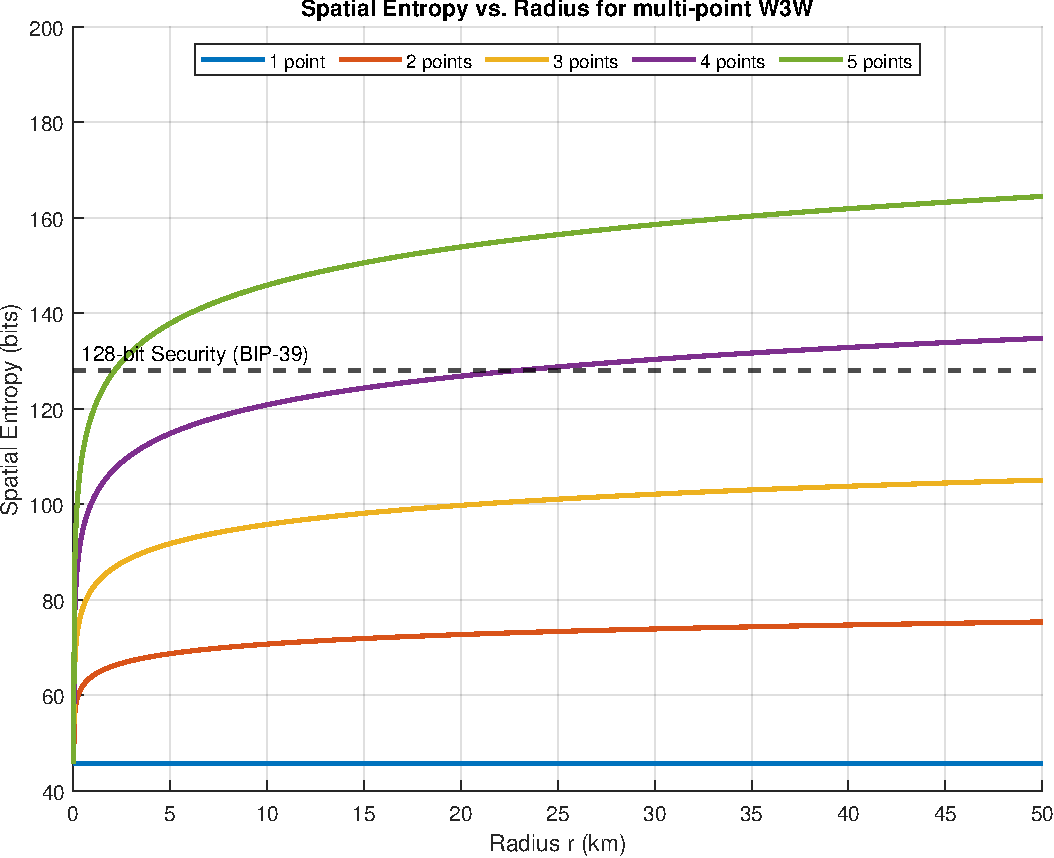
\includegraphics[scale=0.7]{img/w3w_entropy_vs_radius.pdf}
    \caption{Spatial entropy $H_{\mathrm{spatial}}(n,r)$ for multi-point selection under the proximity model.}
    \label{fig:entropy_radius}
\end{figure}

The figure further illustrates that for $n=2$, the achievable entropy saturates below the 128-bit target even under maximal geographic dispersion, as the second point contributes at most the global single-cell entropy.



Table~\ref{tab:raw_radius_entropy} reports the raw entropy limits and the dispersion radius required to reach the 128-bit spatial entropy target defined in Section~\ref{sec:security_evaluation} for increasing numbers of selected points under the proximity model of Section~\ref{sec:clustering}.

\begin{table}[H]
\caption{Raw radius and entropy calculations for multi-point spatial selection under the proximity~model.}
\label{tab:raw_radius_entropy}
\begin{tabularx}{\linewidth}{cCc}
\toprule
\textbf{Points (\boldmath{$n$})} & \textbf{Radius for 128-bit ($r$)} & \textbf{Max Entropy (bits)} \\
 & \textbf{(km)} & \\
\midrule
1 & $\infty$ & 45.70 \\
2 & $4.13 \times 10^{9}$ & 92.69 \\
3 & $2643.86$ & 139.68 \\
4 & $22.79$ & 186.67 \\
5 & $2.12$ & 233.65 \\
\bottomrule
\end{tabularx}
\end{table}

The entropy values in Table~\ref{tab:raw_radius_entropy} are bounded by a maximum feasible dispersion radius corresponding to the Earth’s circumference (approximately $20{,}000$ km). For configurations in which the required radius exceeds this bound, the 128-bit entropy target defined in Section~\ref{sec:security_evaluation} cannot be achieved through geographic dispersion alone. This Earth-scale constraint defines a hard upper limit on the entropy contribution of additional spatial points under the proximity model of Section~\ref{sec:clustering} and explains the saturation behavior observed for small $n$ in Figure~\ref{fig:entropy_radius}.





% =================================================================
% 4.2 HARDWARE BENCHMARKS (Defining R and C)
% =================================================================
\subsection{Key Derivation Cost: Defender Latency vs. Attacker Throughput}
\label{sec:hardware_benchmarks}

To instantiate attacker-adjusted work factors (Section~\ref{sec:security_evaluation}), we measured defender-side latency on CPU and attacker-side throughput on GPU. These measurements instantiate the attacker rates $R_{\text{GPU,hash}}$ and $R_{\text{GPU,Argon2}}(t,m,p)$ in Equations~\eqref{eq:empirical_workfactor_baseline} and~\eqref{eq:empirical_workfactor}.

\subsubsection{Defender-Side Key Derivation Latency}
\label{sec:defender_performance}

A legitimate user (defender) performs a single key derivation event during vault decryption. To quantify the user-visible cost, we measured key derivation latency on the CPU platform specified in Section~\ref{sec:experimental_setup}.

For the unhardened baseline (SHA-256), computational overhead was negligible ($<$0.01\,ms). The BIP-39 baseline, which uses PBKDF2-HMAC-SHA512 with 2048 iterations, exhibited a median latency of 3.57\,ms, a delay that is effectively imperceptible to users. The full latency distribution is reported in Table~\ref{tab:defender_cost_bip39}.

\begin{table}[H]
\caption{Empirical defender benchmark for BIP-39 PBKDF2-HMAC-SHA512 (CPU).}
\label{tab:defender_cost_bip39}
\begin{tabularx}{\linewidth}{CCCCC}
\toprule
\textbf{Iterations} & \textbf{Median (ms)} & \textbf{P90 (ms)} & \textbf{P95 (ms)} & \textbf{P99 (ms)} \\
\midrule
2048 & 3.57 & 3.68 & 3.74 & 4.18 \\
\bottomrule
\end{tabularx}
\end{table}

In contrast, GeoVault applies Argon2id to deliberately impose a hardware-bound delay on key derivation. Table~\ref{tab:argon2_defender_cost} reports defender-side latency as a function of the Argon2id memory parameter $m$ (with $t=1$ and $p=1$). Configurations up to 1024\,MiB remain within a few seconds and are suitable for interactive use, whereas extreme configurations at 16-32\,GiB incur minute-scale delays consistent with archival or cold-storage usage.

\begin{table}[H]
\caption{Empirical Argon2id CPU latency for single invocation ($k=1$, $t=1$, $p=1$, $n=50$ reps).} 
\label{tab:argon2_defender_cost}
\begin{tabularx}{\linewidth}{lm{2.1cm}<{\raggedleft}m{2.1cm}<{\raggedleft}m{2.4cm}<{\raggedleft}m{2.5cm}<{\raggedleft}}
\toprule
\textbf{Memory Setting} & \textbf{Mean (ms)} & \textbf{\boldmath{$\sigma$} (ms)} & \textbf{P50 (ms)} & \textbf{P95 (ms)} \\
\midrule
64 MiB   & 74.0        & 5.2         & 72.4        & 87.1        \\
256 MiB  & 303.2       & 3.3         & 303.4       & 308.5       \\
1024 MiB & 1234.9   & 47.1        & 1219.8   & 1391.5   \\
8192 MiB & 10{,}534.3  & 620.9       & 10{,}269.6  & 12{,}063.0  \\
\bottomrule

\end{tabularx}
\noindent{\footnotesize {CV\,$=$\,3.0--7.0\% (memory bandwidth jitter under OS scheduling; see text).}}
\end{table}

\paragraph*{Consumer Hardware Extrapolation}
{The latencies in Table~\ref{tab:argon2_defender_cost} were measured on a server-class platform (Intel Xeon Gold 6338, quad-channel DDR4, $\approx$204\,GB/s peak memory bandwidth). Since Argon2id throughput is dominated by memory bandwidth rather than compute, defender latency scales approximately inversely with available bandwidth~\cite{7467361}. A typical consumer laptop CPU (e.g., Intel Core i7 12th-generation with dual-channel DDR5~\cite{JEDEC2020DDR5}) delivers approximately 50\% of the Xeon Gold 6338 peak bandwidth, yielding an estimated scaling factor of $\approx$$2\times$. Mobile devices (e.g., ARM Cortex-X class SoC with LPDDR5x, $\approx$$65$\,GB/s peak bandwidth~\cite{JEDEC2022LPDDR5x}) deliver approximately 32\% of the server platform bandwidth, yielding a scaling factor of $\approx$$4\times$ and an estimated latency of $\approx$$4.9$\,s at $m=1024$\,MiB---within a tolerable range for infrequent cold-storage key derivation. Memory tiers above $m=1024$\,MiB may exceed the available RAM on many smartphones (typically 8--12\,GiB) and should not be used on mobile devices without verifying available system memory. Table~\ref{tab:argon2_defender_cost_consumer} reports the projected latency for all evaluated memory tiers across defender hardware classes.}

\begin{table}[H]
\caption{Projected Argon2id defender latency on consumer and mobile hardware ($t=1$, $p=1$, $k=1$). Laptop estimate uses a $\approx$$2\times$ bandwidth scaling factor; smartphone estimate uses a $\approx$$4\times$ scaling factor relative to the Intel Xeon Gold 6338 server platform. Entry marked with --- exceeds typical smartphone RAM.}
\label{tab:argon2_defender_cost_consumer}
\begin{tabularx}{\linewidth}{lm{3.4cm}<{\raggedleft}m{3.4cm}<{\raggedleft}m{3.4cm}<{\raggedleft}}
\toprule
\textbf{Memory \boldmath{$m$}} & \textbf{T\textsubscript{server} (s)} & \textbf{T\textsubscript{laptop} (s)} & \textbf{T\textsubscript{phone} (s)} \\
\midrule
64\,MiB      & 0.07  & 0.15          & 0.28          \\
256\,MiB     & 0.30  & 0.63          & 1.20          \\
1024\,MiB & 1.23  & \textbf{{2.6}}  & \textbf{{4.9}}  \\
8192\,MiB & 10.5  & 22.1          & ---           \\
\bottomrule
\end{tabularx}

\noindent{\footnotesize {Reference configuration ($m=1024$\,MiB, bold) is within tolerable range on both laptop and phone for cold-storage~use.}}
\end{table}

{Table~\ref{tab:argon2_defender_cost} reports single-invocation latency ($k=1$). When the user applies KDF chaining at depth $k$ (Equation~\eqref{eq:kdf_chaining}), the total key derivation time scales linearly as $T_\text{CPU}(k) = k \cdot T_\text{CPU}^{(1)}$. Table~\ref{tab:kchain_empirical} reports empirically measured chain latency for all powers-of-two depths at the \mbox{$m=1024$\,MiB} reference configuration ($n=50$ reps each). The measured ratios $T(k)/(k\cdot T(1))$ lie within~2\% of unity across all $k\in\{1,2,4,8,16,32,64\}$, confirming linearity.}

\begin{table}[H]
\caption{KDF chain latency by depth ($m=1024$\,MiB, $t=1$, $p=1$, $n=50$ reps each). All rows empirically measured; ratio $= T(k)/(k\cdot T(1))$ confirms linearity to within~2\%.}
\label{tab:kchain_empirical}
\begin{tabularx}{\linewidth}{m{3cm}<{\raggedleft}m{3cm}<{\raggedleft}m{3cm}<{\raggedleft}m{3cm}<{\raggedleft}}
\toprule
\textbf{Depth \boldmath{$k$}} & \textbf{Mean (s)} & \textbf{\boldmath{$\sigma$} (s)} & \textbf{Ratio} \\
\midrule
 1 &  1.255 & 0.006 & 1.000 \\
 2 &  2.526 & 0.046 & 1.006 \\
 4 &  5.051 & 0.053 & 1.006 \\
 8 & 10.099 & 0.098 & 1.007 \\
16 & 20.281 & 0.221 & 1.011 \\
32 & 41.200 & 0.651 & 1.027 \\
64 & 82.499 & 1.213 & 1.029 \\
\bottomrule
\end{tabularx}
\noindent{\footnotesize {$n=50$ reps each; ratio $= T(k)/(k\cdot T(1))$; $T(1)=1.255$\,s.}}
\end{table}

{From the attacker's perspective, the serial data dependency of the chaining construction (Equation~\eqref{eq:kdf_chaining}) prevents evaluating multiple rounds in parallel for a single candidate: call $i+1$ cannot begin until the output of call $i$ is known. Direct GPU measurement of k-chained throughput is not possible with standard benchmarking tools, as Hashcat (mode 34000)
supports only single, independent Argon2id invocations and has no mechanism to chain outputs as inputs within a single pass. The attacker throughput under k-chaining is therefore derived analytically as $R_\text{GPU}^{(k)} = R_\text{GPU}^{(1)}/k$. This derivation is validated by the CPU linearity measurements in Table~\ref{tab:kchain_empirical}: the empirical ratios $T(k)/(k \cdot T(1))$ lie in the range $[1.000, 1.029]$ for all $k \in \{1,2,4,8,16,32,64\}$, confirming that each additional chain call adds at least as much latency as the first. Because the true per-chain overhead on the GPU is at least as large as on the CPU (both are dominated by memory-bound Argon2id computation), using $R_\text{GPU}^{(1)}/k$ as the attacker rate overestimates the attacker by at most 3\% at $k=64$. All time-to-compromise values derived from this formula are therefore conservative lower bounds.}


\subsubsection{Attacker-Side Guess Throughput}
\label{sec:attacker_performance}

Attacker-side capabilities were benchmarked using Hashcat under the attacker model defined in Section~\ref{sec:security_evaluation}. We distinguish between \emph{compute-bound} primitives, which scale efficiently with GPU parallelism (SHA-256, PBKDF2), and \emph{memory-bound} primitives, for which throughput is fundamentally constrained by available high-bandwidth memory (Argon2id).

\paragraph*{BIP-39 Throughput (PBKDF2)}
For linguistic mnemonics, an offline attacker evaluates candidate phrases using PBKDF2-HMAC-SHA512 as specified by the BIP-39 standard. Hashcat benchmarks were scaled to the full 2048-iteration configuration. The measured sustained throughput is reported in Table~\ref{tab:attacker_cost}:
\[
R_{2048} \approx 6.40 \times 10^{5} \ \text{H/s}.
\]

\begin{table}[H]
\caption{Empirical attacker benchmark for BIP-39 PBKDF2-HMAC-SHA512 (GPU).}
\label{tab:attacker_cost}
\begin{tabularx}{\linewidth}{C CC}
\toprule
\textbf{Runs (\boldmath{$n_{\text{rep}}$})} & \textbf{Mean Time per Guess} & \textbf{Throughput \boldmath{$R_{2048}$} (H/s)} \\
\midrule
30 & $1.56~\upmu\mathrm{s}$ & $6.40 \times 10^{5}$ \\
\bottomrule
\end{tabularx}
\end{table}

\paragraph*{Fast Hash Throughput (SHA-256)}
For unhardened secrets verified using a single cryptographic hash, the attacker employs raw SHA-256. Benchmarks indicate a sustained throughput of approximately
\[
R_{\text{GPU,hash}} \approx 1.3 \times 10^{7} \ \text{H/s},
\]
with only minor degradation as input length increases. This rate serves as the baseline attacker capability for raw spatial and password-based secrets without computational hardening.

\paragraph*{Argon2id Throughput (Memory-Hard Regime)}
To characterize attacker performance against GeoVault-style hardened secrets, we measured Argon2id throughput across a wide range of memory costs $m$ with fixed parameters $(t=1, p=1)$. Table~\ref{tab:argon2_spectrum} reports the resulting attacker throughput as a function of~$m$.

\begin{table}[H]
\caption{Empirical attacker Argon2id throughput as a function of memory cost $m$ ($t=1$).}
\label{tab:argon2_spectrum}
\begin{tabularx}{\linewidth}{r CCC}
\toprule
\textbf{Memory (MiB)} & \textbf{Median (H/s)} & \textbf{P95 (H/s)} & \textbf{P99 (H/s)} \\
\midrule
64    & 4985.50 & 4988.50 & 4988.50 \\
128   & 2339.00 & 2341.00 & 2341.00 \\
256   & 802.00  & 803.00  & 803.00  \\
512   & 212.00  & 212.00  & 212.00  \\
\midrule
1024  & 53.66   & 53.80   & 53.80   \\
2048  & 13.56   & 13.56   & 13.56   \\
4096  & 2.70    & 2.70    & 2.70    \\
8192  & 0.54    & 0.54    & 0.54    \\
\midrule
16,384 & 0.11    & 0.11    & 0.11    \\
32,768 & 0.03    & 0.03    & 0.03    \\
\bottomrule
\end{tabularx}

\noindent{\footnotesize{GPU throughput is highly deterministic: P95\,$=$\,median for all tiers at or above 2048\,MiB; CV\,$<$\,0.1\% for all rows. No explicit $\sigma$ column is needed for attacker-side measurements.}} 
\end{table}

\clearpage
The results show a sharp, non-linear collapse in attacker throughput as the memory cost approaches and exceeds the GPU’s available VRAM. At $m = 1024$\,MiB, throughput is already reduced by more than five orders of magnitude relative to SHA-256. At 16--32\,GiB, attacker throughput falls below one guess per second, indicating entry into a hardware-capacity regime in which GPU parallelism is no longer exploitable and brute-force attacks become effectively serialized.

\paragraph*{Defender--Attacker Throughput Asymmetry}
{To separate the two primary security axes of GeoVault---memory cost $m$ and spatial dimensionality $n$---and isolate the KDF's standalone contribution, we define the \emph{GPU throughput advantage}:}
\begin{equation}
    \eta(m) = R_\text{GPU}(m) \cdot T_\text{CPU}(m)
    \label{eq:eta}
\end{equation}
where $R_\text{GPU}(m)$ is the attacker GPU guess rate (H/s) and $T_\text{CPU}(m)$ is the defender CPU key derivation latency (s). The quantity $\eta(m)$ is the number of attacker guesses that can be tested in the time it takes the legitimate user to perform one key derivation. Its value as a design metric lies in decomposing the security problem: $\eta$ characterizes the residual attacker advantage after $m$ is fixed, independently of the search space size set by $n$. Table~\ref{tab:eta} reports $\eta$ for the measured Argon2id tiers.


\begin{table}[H]
\caption{GPU throughput advantage $\eta(m) = R_\text{GPU}(m)\cdot T_\text{CPU}(m)$: attacker guesses per one defender authentication event. KDF chaining depth $k$ does not change $\eta$; only $m$ drives it downward. Defender latencies from Table~\ref{tab:argon2_defender_cost}; attacker rates from Table~\ref{tab:argon2_spectrum}.}
\label{tab:eta}
\begin{tabularx}{\linewidth}{lm{3.3cm}<{\raggedleft}m{3.3cm}<{\raggedleft}m{3.3cm}<{\raggedleft}}
\toprule
\textbf{Memory \boldmath{$m$}} & \textbf{\boldmath{$R_\text{GPU}$} (H/s)} & \textbf{\boldmath{$T_\text{CPU}$} (s)} & \textbf{\boldmath{$\eta$}} \\
\midrule
64\,MiB       & 4985  & 0.074       & 369           \\
256\,MiB      & 802   & 0.303       & 243           \\
1024\,MiB  & 53.7  & 1.235       &  66           \\
8192\,MiB  & 0.54  & 10.53       & 5.7           \\
32{,}768\,MiB & 0.03  & $\approx$82 & $\approx$2.5  \\
\bottomrule
\end{tabularx}

\noindent{\footnotesize{$k$-chaining leaves $\eta$ unchanged; spatial points $n$ add entropy without affecting $\eta$.}}
\end{table}


Two structural properties follow directly from this decomposition.
First, \emph{KDF chaining depth $k$ leaves $\eta$ unchanged.} Since $R_\text{GPU}^{(k)} = R_\text{GPU}^{(1)}/k$ and $T_\text{CPU}^{(k)} = k\cdot T_\text{CPU}^{(1)}$, the product $\eta(m,k) = R_\text{GPU}^{(1)}\cdot T_\text{CPU}^{(1)} = \eta(m,1)$. Chaining raises the absolute cost of each guess symmetrically but cannot change the ratio; it belongs to the $m$-axis, not to a third independent axis.
Second, \emph{spatial dimensionality $n$ is orthogonal to $\eta$.} Adding a spatial point multiplies the search space by $\approx\!2^{26.8}$ per point (Table~\ref{tab:raw_radius_entropy}) without affecting either $R_\text{GPU}$ or $T_\text{CPU}$. Consequently, $\eta$ can be read directly as the fraction of the security budget that must be covered by the search space rather than by the KDF: at $\eta = 66$, the search space must be at least $66\,	imes$ larger than the KDF work factor to clear any given security threshold, a condition met with wide margin at $n \geq 3$.



\paragraph*{Argon2id Throughput Under KDF Chaining}
{Table~\ref{tab:argon2_kchain_attacker} reports derived attacker throughput under KDF chaining at the $m=1024$\,MiB reference tier, computed as $R_\text{GPU}^{(k)} = R_\text{GPU}^{(1)}/k$ with $R_\text{GPU}^{(1)} = 53.7$\,H/s (Section~\ref{sec:defender_performance}; CPU linearity validates the formula, Table~\ref{tab:kchain_empirical}; all time-to-compromise values are conservative lower bounds).}

\begin{table}[H]
\setlength{\tabcolsep}{12.56mm}
\caption{Derived attacker Argon2id throughput under KDF chaining ($m=1024$\,MiB, $t=1$, $p=1$). Values computed as $R^{(k)} = R^{(1)}/k$ with $R^{(1)}=53.7$\,H/s; conservative upper bound on true attacker rate (CPU linearity ratios $\leq 1.029$, Table~\ref{tab:kchain_empirical}).}
\label{tab:argon2_kchain_attacker}
\begin{tabularx}{\linewidth}{rrl}
\toprule
\textbf{Depth \boldmath{$k$}} & \textbf{\boldmath{$R^{(k)}$} (H/s)} & \textbf{Basis} \\
\midrule
 1 & 53.70 & measured \\
 2 & 26.85 & derived ($R^{(1)}/k$) \\
 4 & 13.43 & derived \\
 8 &  6.71 & derived \\
16 &  3.36 & derived \\
32 &  1.68 & derived \\
64 &  0.84 & derived \\
\bottomrule
\end{tabularx}

{\footnotesize CPU ratios confirm true $R^{(k)} \leq R^{(1)}/k$; time-to-compromise values are lower bounds.}
\end{table}


\paragraph*{ASIC Attack Resistance}
{A natural concern is whether purpose-built application-specific integrated circuits (ASICs) could exceed the measured GPU attacker throughput and invalidate the work factor estimates. For Argon2id, this is fundamentally limited by the memory bandwidth bottleneck rather than compute throughput. The Argon2 specification formally establishes that any implementation allocating less than the nominal memory $m$ incurs an exponential time penalty through mandatory data-dependent recomputation, precluding any space--time trade-off~\cite{7467361}. A hypothetical Argon2id ASIC must therefore provision high-bandwidth memory comparable to the target GPU; savings come only from eliminating general-purpose execution overhead in the compute fabric, which the Argon2 designers estimate yields a practical speedup of approximately $2$--$4\times$ over GPU-class hardware for realistic ASIC implementations~\cite{7467361,Wetzels2016}. Applying a conservative $10\times$ ASIC advantage to the reference attacker rate ($R_{\text{GPU}} = 53.7$\,H/s at $m=1024$\,MiB) yields $R_{\text{ASIC}} \leq 537$\,H/s. This reduces all reported Argon2id attacker-adjusted work factors by at most $\log_2(10) \approx 3.3$\,bits. At $n=3$ spatial points, the baseline work factor exceeds $10^{39}$\,s (Super Secure zone, Section~\ref{sec:defense_in_depth});
a 3.3-bit reduction leaves it at $>$$10^{38}$\,s, well within the same zone. For the $n=1$ case at $m=1024$\,MiB, the work factor remains in the Human-Scale Secure zone even under this pessimistic ASIC bound. The GPU benchmark therefore provides a conservative upper bound on adversarial throughput under memory-hard protection, and ASIC-specific threats do not materially alter the security conclusions of Sections~\ref{sec:hardened_analysis}--\ref{sec:defense_in_depth}.}

\subsection{Baseline Brute-Force Resistance Under Fast Hashing}
\label{sec:unhardened_analysis}

We analyze the security of linguistic and spatial mnemonics in their \emph{raw} state, assuming an attacker utilizes a standard fast hash primitive (SHA-256) without memory-hard protection. In this setting, entropy is treated as a fixed input parameter, and security is evaluated exclusively via the attacker-adjusted work factor $\mathcal{W}$ defined in Equation~\eqref{eq:work_factor_attacker}. Following Section~\ref{sec:security_evaluation}, we categorize security into three qualitative zones based on $\mathcal{W}$: Insecure ($<$$10^{10}$ s), Human-Scale Secure ($10^{10}$--$10^{32}$ s), and Super Secure ($\ge$$10^{32}$ s).

\subsubsection{Brute-Force Resistance of Linguistic Secrets}

For typical human passwords, brute-force resistance under fast hashing is determined by the effective entropy implied by alphabet size and length. As established in Section~\ref{sec2.1}, human-chosen passwords frequently collapse to approximately $20$ bits of effective entropy under adaptive guessing models. Using the baseline attacker work factor formulation for fast hashing given in Equation~\eqref{eq:empirical_workfactor_baseline}, the expected time to compromise such a secret is
\begin{equation}
\mathcal{W}_{\text{password}} \approx \frac{2^{20}}{1.32 \times 10^7} \approx 0.08 \ \text{s}.
\end{equation}

To transition from the Insecure zone into the Super Secure (BIP-39) regime without computational hardening, a user would need to memorize a truly random ASCII-94 string. The required string length $L$ follows directly from the entropy target:
\begin{equation}
L = \left\lceil \frac{128}{\log_2(94)} \right\rceil = \left\lceil \frac{128}{6.55} \right\rceil = 20 \ \text{characters}.
\end{equation}
Such strings (e.g., \texttt{7\&y\#B9@q!x2\$LpZ*5mW1})
substantially exceed typical human cognitive limits for reliable recall, illustrating the well-known usability barrier of high-entropy linguistic secrets.

\subsubsection{Brute-Force Resistance of Spatial Secrets}

In contrast, spatial mnemonics exhibit substantially higher baseline brute-force resistance due to their higher effective entropy. Applying the same baseline work factor model of Equation~\eqref{eq:empirical_workfactor_baseline} to a single unhardened What3Words location ($n=1$) yields an expected attack time of approximately $4.34 \times 10^{6}$ s (about $50$ days). While this remains within the Insecure zone, it represents roughly a seven-order-of-magnitude improvement over typical human-chosen passwords.

Figure~\ref{fig:resultsNoKDF} visualizes this equivalence in brute-force resistance between spatial and linguistic secrets across the three defined security zones under fast hashing.

\vspace{-10pt}
\begin{figure}[H]
    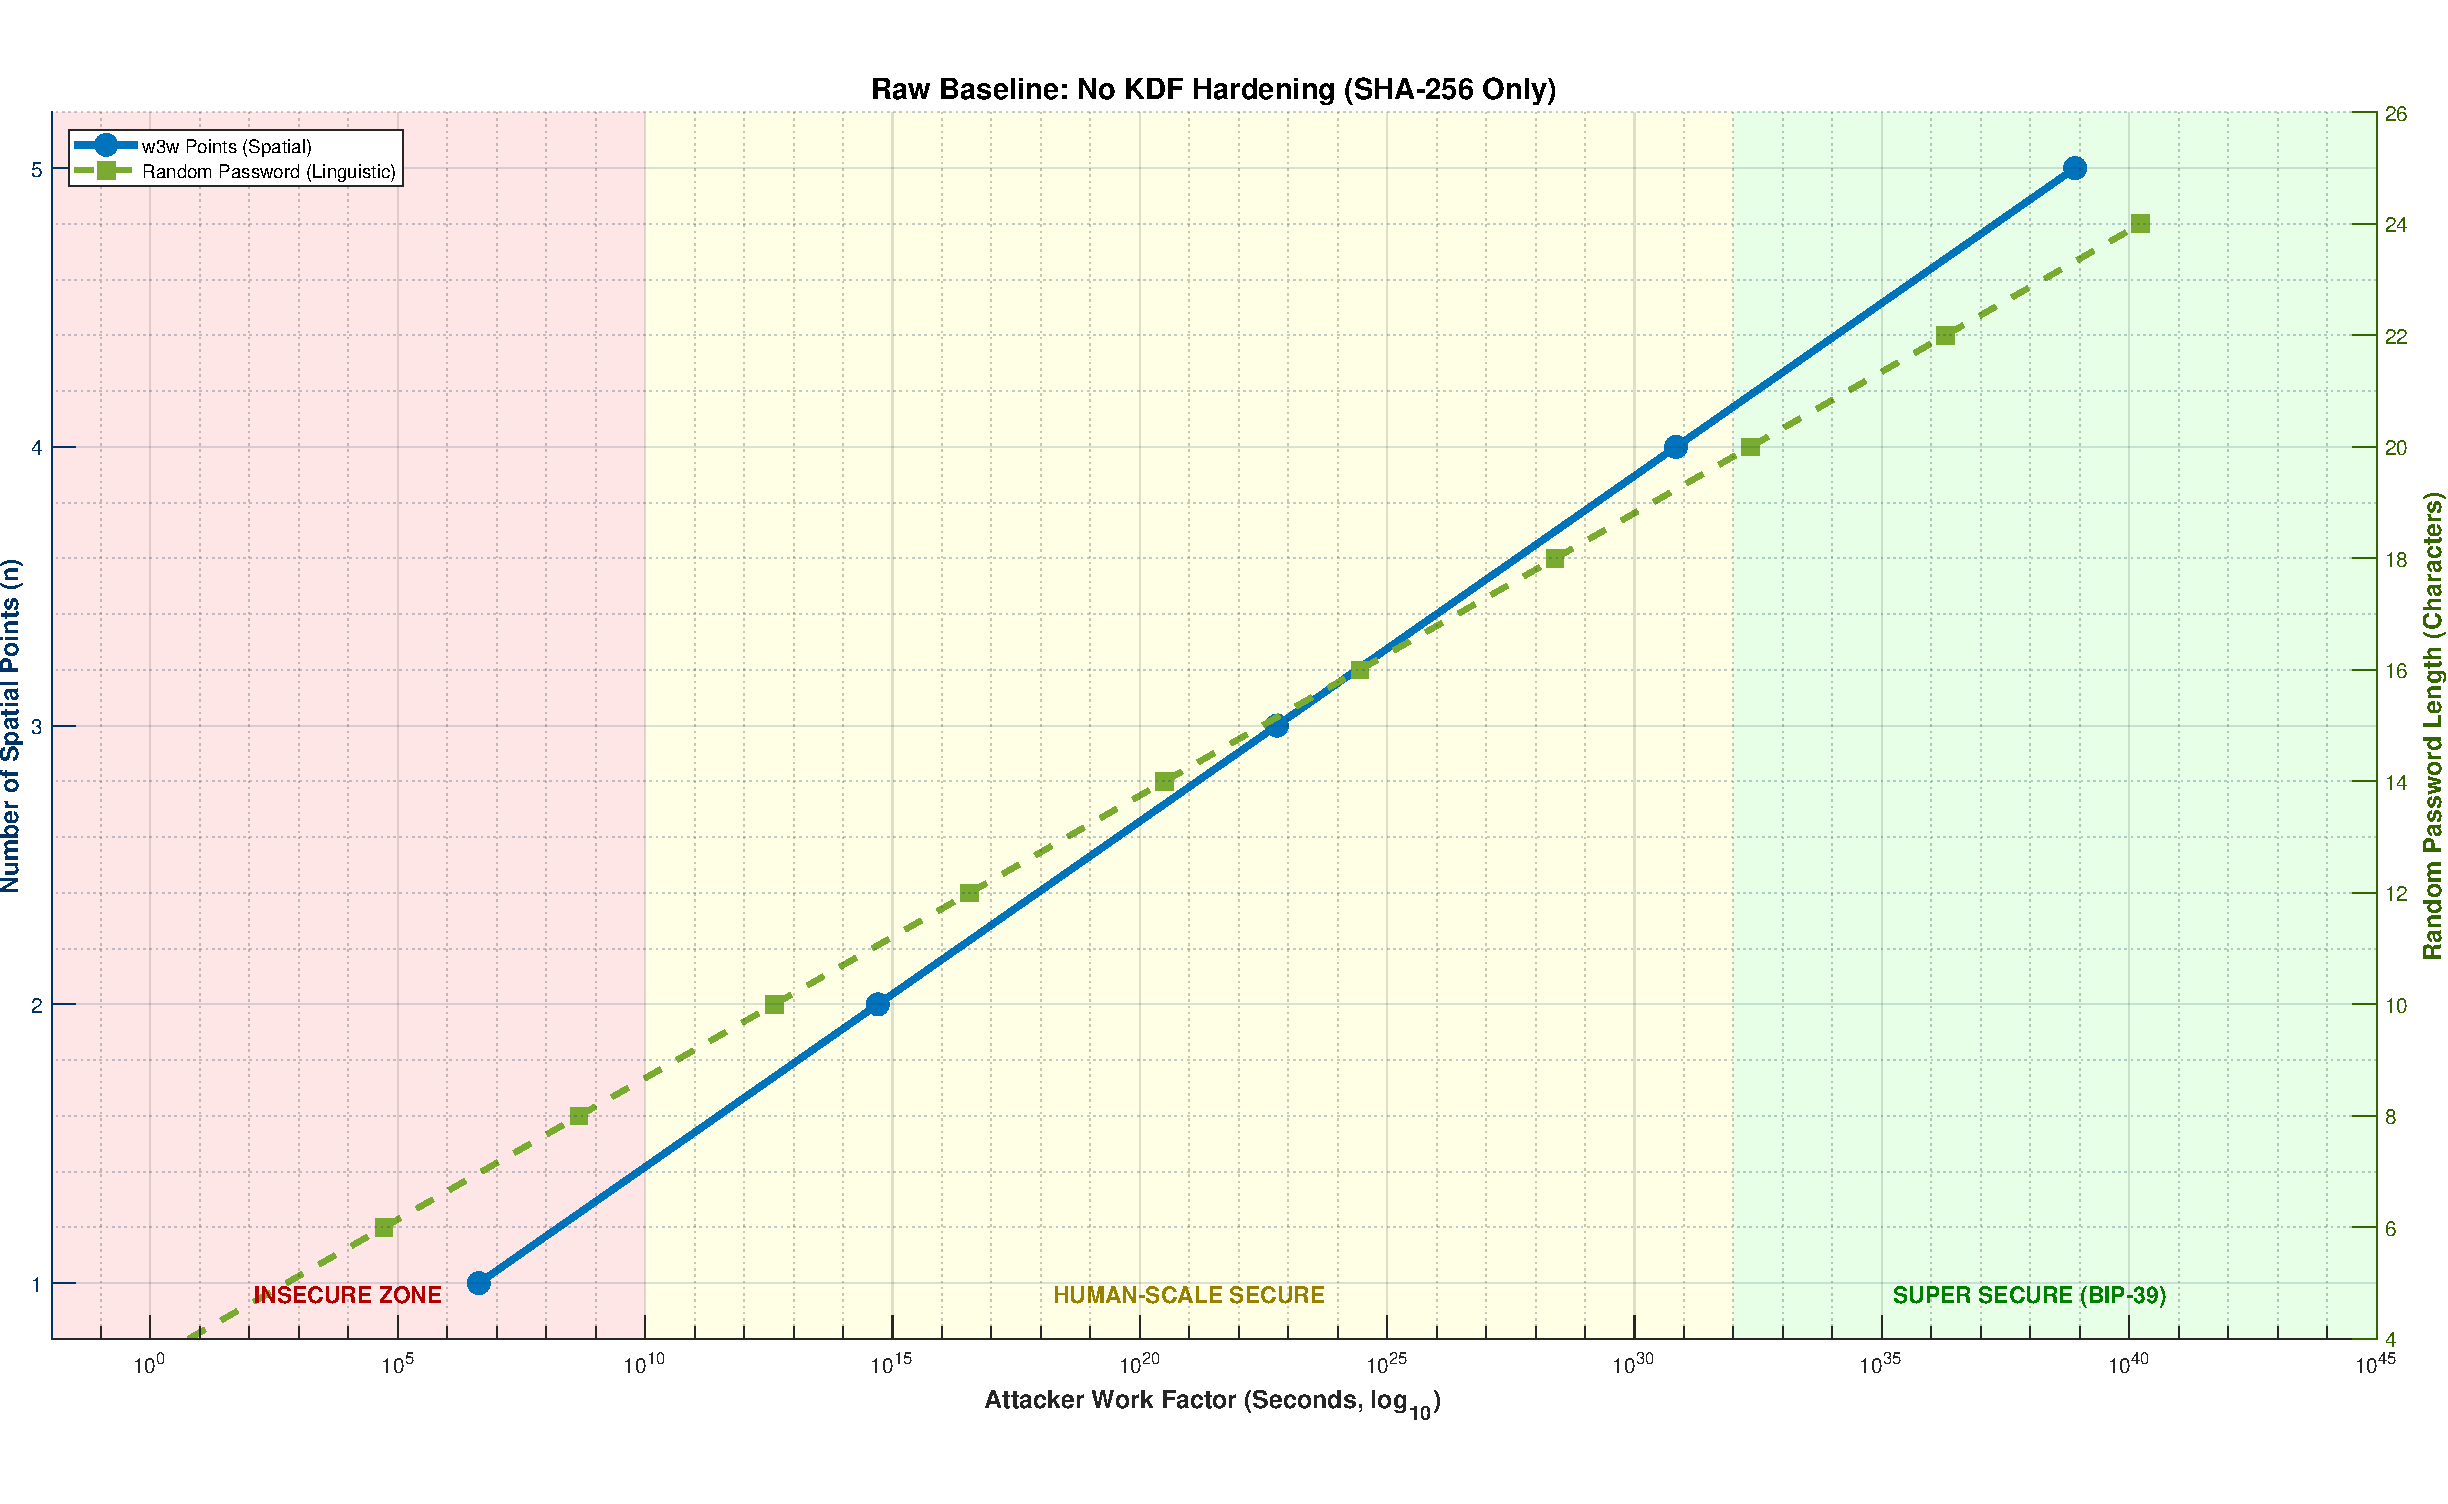
\includegraphics[width=0.98\textwidth]{img/resultsNoKDF_II.pdf}
    \vspace{-10pt}
    \caption{Raw baseline brute-force resistance under SHA-256 hashing: spatial points versus random password length. Shaded regions indicate the defined security zones: Insecure (red), Human-Scale Secure (yellow), and Super Secure/BIP-39 (green).}
    \label{fig:resultsNoKDF}
\end{figure}

As the number of spatial points increases, the total search space expands sufficiently for spatial mnemonics to exceed the 128-bit security threshold even without computational hardening. Table~\ref{tab:w3w_breakeven} reports the geographic dispersion required for the baseline work factor of Equation~\eqref{eq:empirical_workfactor_baseline} to enter the Super Secure regime under SHA-256.

These results highlight the fundamental advantage of spatial mnemonics under fast hashing: achieving super-secure brute-force resistance requires either memorizing approximately $20$ random characters (cognitively impractical) or recalling a small number of geographically meaningful locations (cognitively feasible).


\begin{table}[H]
\caption{Breakeven analysis required spatial dispersion to achieve 128-bit brute-force resistance using SHA-256.}
\label{tab:w3w_breakeven}
\begin{tabularx}{\linewidth}{cClC}
\toprule
\textbf{Points (\boldmath{$n$})} & \textbf{Radius (\boldmath{$r$})} & \textbf{Feasibility} & \textbf{Security Zone} \\
\midrule
1 & Impossible & Exceeds Earth's area & Insecure \\
2 & Impossible & Exceeds Earth's area & Insecure \\
3 & $5396$ km & Continental scale & Human-Scale \\
\textbf{4} & \textbf{36.4 km} & \textbf{City scale} & \textbf{Super Secure} \\
5 & 3.0 km & Neighborhood scale & Super Secure \\
\bottomrule
\end{tabularx}
\end{table}


\subsection{Brute-Force Resistance Under Memory-Hard KDFs}
\label{sec:hardened_analysis}

We analyze the impact of memory-hard key derivation on brute-force resistance by applying Argon2id across a wide range of memory costs, including extreme configurations (16~GiB and 32~GiB) that approach or exceed the physical VRAM limits of professional-grade GPU hardware. As in the previous subsection, entropy is treated as a fixed input parameter, and security is evaluated via the attacker-adjusted work factor $\mathcal{W}$ defined in Equation~\eqref{eq:work_factor_attacker}. Throughout this analysis, BIP-39--equivalent security is defined as a time-to-compromise exceeding $10^{32}$ s, consistent with Section~\ref{sec:security_evaluation}.

Table~\ref{tab:spectrum_comparison} reports the corresponding time-to-compromise values for a representative linguistic secret (approximately $20$ bits of effective entropy) and a single spatial point ($n=1$, approximately $45.7$ bits), derived from the attacker throughput measurements reported in Section~\ref{sec:hardware_benchmarks}. All values are computed using the Argon2id work factor model of Equation~\eqref{eq:empirical_workfactor}.


\begin{table}[H]
\caption{Time-to-compromise
 under Argon2id hardening for linguistic ($\approx$20 bits) and single-point spatial secrets ($n=1$, $\approx$45.7 bits).}
\label{tab:spectrum_comparison}
\begin{tabularx}{\linewidth}{r CCC}
\toprule
\textbf{Memory} & \textbf{Attacker Rate} & \textbf{Password Time} & \textbf{Spatial Time (\boldmath{$n=1$})} \\
\textbf{(MiB)} & \textbf{(\boldmath{$R$})} & \textbf{(\boldmath{$\approx$20} bits)} & \textbf{(\boldmath{$\approx$45.7} bits)} \\
\midrule
64    & 4986 H/s & 3.5 min & $360$ years \\
128   & 2339 H/s & 7.5 min & $768$ years \\
256   & 802 H/s  & 22.0 min & $2240$ years \\
512   & 212 H/s  & 1.4 h & $8480$ years \\
1024  & 53.7 H/s & 5.4 h & $33{,}400$ years \\
2048  & 13.6 H/s & 21.5 h & $132{,}000$ years \\
4096  & 2.7 H/s  & 4.5 days & $665{,}000$ years \\
8192  & 0.54 H/s & 22.5 days & $3.3$ million years \\
\noalign{\hrule height 0.5pt}
\rowcolor[gray]{0.9} 16,384 (16 G) & 0.115 H/s & 105 days & $15.5$ million years \\
\rowcolor[gray]{0.9} 32,768 (32 G) & 0.026 H/s & 1.2 years & $68.6$ million years \\
\noalign{\hrule height 1.0pt}
\end{tabularx}
\end{table}


The results demonstrate a pronounced hardware-enforced non-linearity in attacker cost as the Argon2id memory parameter approaches the GPU’s available VRAM. In particular, at 16–32~GiB, attacker throughput collapses due to the inability to parallelize memory-bound computations, effectively serializing brute-force attempts.

For linguistic secrets, even extreme 32~GiB hardening—while imposing substantial defender-side latency—remains vulnerable to compromise on the order of one year under the attacker model considered. In contrast, a single spatial point ($n=1$) under the same hardening parameters achieves an expected time-to-compromise of approximately $6.9 \times 10^{7}$ years. Although this remains below the $10^{32}$ second BIP-39 threshold, it comfortably exceeds human and geological timescales, corresponding to the Human-Scale+ regime.


\clearpage
These results confirm that combining spatial entropy with high-memory KDF hardening fundamentally alters the brute-force landscape by enforcing hardware-level constraints on the attacker, thereby breaking the traditional security–usability trade-off observed for linguistic secrets.

% =================================================================
% 5.5 KDF CHAINING DEPTH k
% =================================================================
\subsection{Effect of KDF Chaining Depth on Brute-Force Resistance}
\label{sec:kchain_analysis}
\label{sec:kchain_spectrum}

{KDF chaining (Equation~\eqref{eq:kdf_chaining}) provides a user-controlled work factor multiplier that scales both sides of the security equation linearly. Because each invocation reuses the full $m$-byte memory footprint and the serial data dependency prevents per-candidate parallelism, attacker throughput drops to $R_\text{GPU}^{(k)} = R_\text{GPU}^{(1)} / k$ (Table~\ref{tab:argon2_kchain_attacker}; conservative upper bound-CPU linearity ratios $\leq 1.029$ confirm that the true attacker rate satisfies $R^{(k)} \leq R^{(1)}/k$) while defender latency grows to $T_\text{CPU}(k) = k \cdot T_\text{CPU}^{(1)}$ (Table~\ref{tab:kchain_empirical}). Table~\ref{tab:k_chaining_effect} quantifies this trade-off at two memory tiers ($m=1024$\,MiB and $m=4096$\,MiB); all attacker time-to-compromise values are lower bounds on actual security.}

\begin{table}[H]
\setlength{\tabcolsep}{4.23mm}
\caption{Effect of KDF chaining depth $k$ on attacker time-to-compromise and defender wait time, at $m=1024$\,MiB ($R^{(1)}\approx53.7$\,H/s, $T_\text{CPU}^{(1)}\approx1.3$\,s) and $m=4096$\,MiB ($R^{(1)}\approx2.70$\,H/s, $T_\text{CPU}^{(1)}\approx10$\,s). Defender wait = $k\times T_\text{CPU}^{(1)}$; attacker columns derived from $R(k)=R(1)/k$. Cell shading indicates security zone.}
\label{tab:k_chaining_effect}
\begin{tabularx}{\linewidth}{rrrrrr}
\toprule
\textbf{Chaining} & \multicolumn{2}{c}{\textbf{Defender Wait}} & \textbf{Password} & \multicolumn{2}{c}{\textbf{Spatial, \boldmath{$n=1$ ($\approx$}45.7 bits)}} \\
\cmidrule{2-6}
\textbf{Depth \boldmath{$k$}} & \textbf{1\,GiB} & \textbf{4\,GiB} & \textbf{($\approx$20 bits)} & \textbf{1\,GiB} & \textbf{4\,GiB} \\
\noalign{\hrule height 0.5pt}
 1 &  1.3\,s &  10\,s & \cellcolor{insecure}5.4\,h    & \cellcolor{humanscale}$3.3\times10^{4}$\,yr & \cellcolor{humanscale}$6.7\times10^{5}$\,yr \\
 2 &  2.5\,s &  20\,s & \cellcolor{insecure}10.8\,h   & \cellcolor{humanscale}$6.6\times10^{4}$\,yr & \cellcolor{humanscale}$1.3\times10^{6}$\,yr \\
 4 &  5.1\,s &  40\,s & \cellcolor{insecure}21.7\,h   & \cellcolor{humanscale}$1.3\times10^{5}$\,yr & \cellcolor{humanscale}$2.7\times10^{6}$\,yr \\
 8 & 10.1\,s & 1.3\,min & \cellcolor{insecure}1.8\,days  & \cellcolor{humanscale}$2.6\times10^{5}$\,yr & \cellcolor{humanscale}$5.4\times10^{6}$\,yr \\
16 & 20.3\,s & 2.7\,min & \cellcolor{insecure}3.6\,days  & \cellcolor{humanscale}$5.3\times10^{5}$\,yr & \cellcolor{humanscale}$1.1\times10^{7}$\,yr \\
32 & 41.2\,s & 5.3\,min & \cellcolor{insecure}7.2\,days  & \cellcolor{humanscale}$1.1\times10^{6}$\,yr & \cellcolor{humanscale}$2.1\times10^{7}$\,yr \\
64 & 82.5\,s & 10.7\,min & \cellcolor{insecure}14.5\,days & \cellcolor{humanscale}$2.1\times10^{6}$\,yr & \cellcolor{humanscale}$4.3\times10^{7}$\,yr \\
\noalign{\hrule height 1.0pt}

\end{tabularx}
\noindent{\footnotesize Password column uses 1\,GiB attacker rate; 4\,GiB values are $20\times$ larger but remain in the Insecure zone.}
\end{table}

{Three conclusions follow. First, for low-entropy linguistic secrets ($\approx$20 bits), chaining provides no practical rescue at either memory tier: even at $k=64$, the expected time-to-compromise remains below $10^{10}$\,s (Insecure zone) because the entropy deficit is too large for a linear multiplier to overcome. Second, for single-point spatial secrets, increasing $m$ from 1\,GiB to 4\,GiB multiplies the work factor by $\approx\!20\times$ at every $k$ level-a direct consequence of the $20\times$ reduction in attacker throughput---yet all entries remain in the Human-Scale Secure zone. No combination of $k$ and $m$ evaluated here lifts an $n=1$ configuration to the Super Secure zone;
 that threshold requires additional spatial points (Section~\ref{sec:defense_in_depth}). Third, the 4\,GiB column makes the defender cost explicit: the 10\,s per-invocation wait is acceptable for cold-storage or archive scenarios, but is above the interactive 2\,s budget at $k>1$. Users with a strict latency constraint should prefer $m=1024$\,MiB with higher $k$, or add a second spatial point, over increasing $m$ to 4\,GiB.}


% =================================================================
% 5.6 KDF CHAINING AND MULTI-POINT SELECTION (BIP-39 EQUIVALENCE)
% =================================================================
\subsection{Brute-Force Resistance via Combined Spatial and Computational Hardening}
\label{sec:defense_in_depth}

%\remove{We analyze the combined effect of spatial multi-point selection and memory-hard key derivation on brute-force resistance.}
{We analyze the joint effect of KDF chaining depth $k$, multi-point spatial selection, and memory-hard key derivation on brute-force resistance. Since each factor independently multiplies the attacker work factor, their combination yields compounding security gains without additional memorization burden.} As in the preceding subsections, spatial entropy is treated as a fixed input parameter (Section~\ref{sec:clustering}), and security is evaluated exclusively via the attacker-adjusted work factor $\mathcal{W}$ defined in Equation~\eqref{eq:work_factor_attacker}.

Figure~\ref{fig:hardening_spectrum} visualizes the combined effect: the Y-axis encodes the number of spatial points $n$ (top panel) or password length in characters (bottom panel), the X-axis is the attacker work factor on a log scale, and each colored line corresponds to a different Argon2id memory tier. The figure instantiates Equation~\eqref{eq:empirical_workfactor} using the empirically measured throughput values of Section~\ref{sec:hardware_benchmarks}.

\begin{figure}[H]
    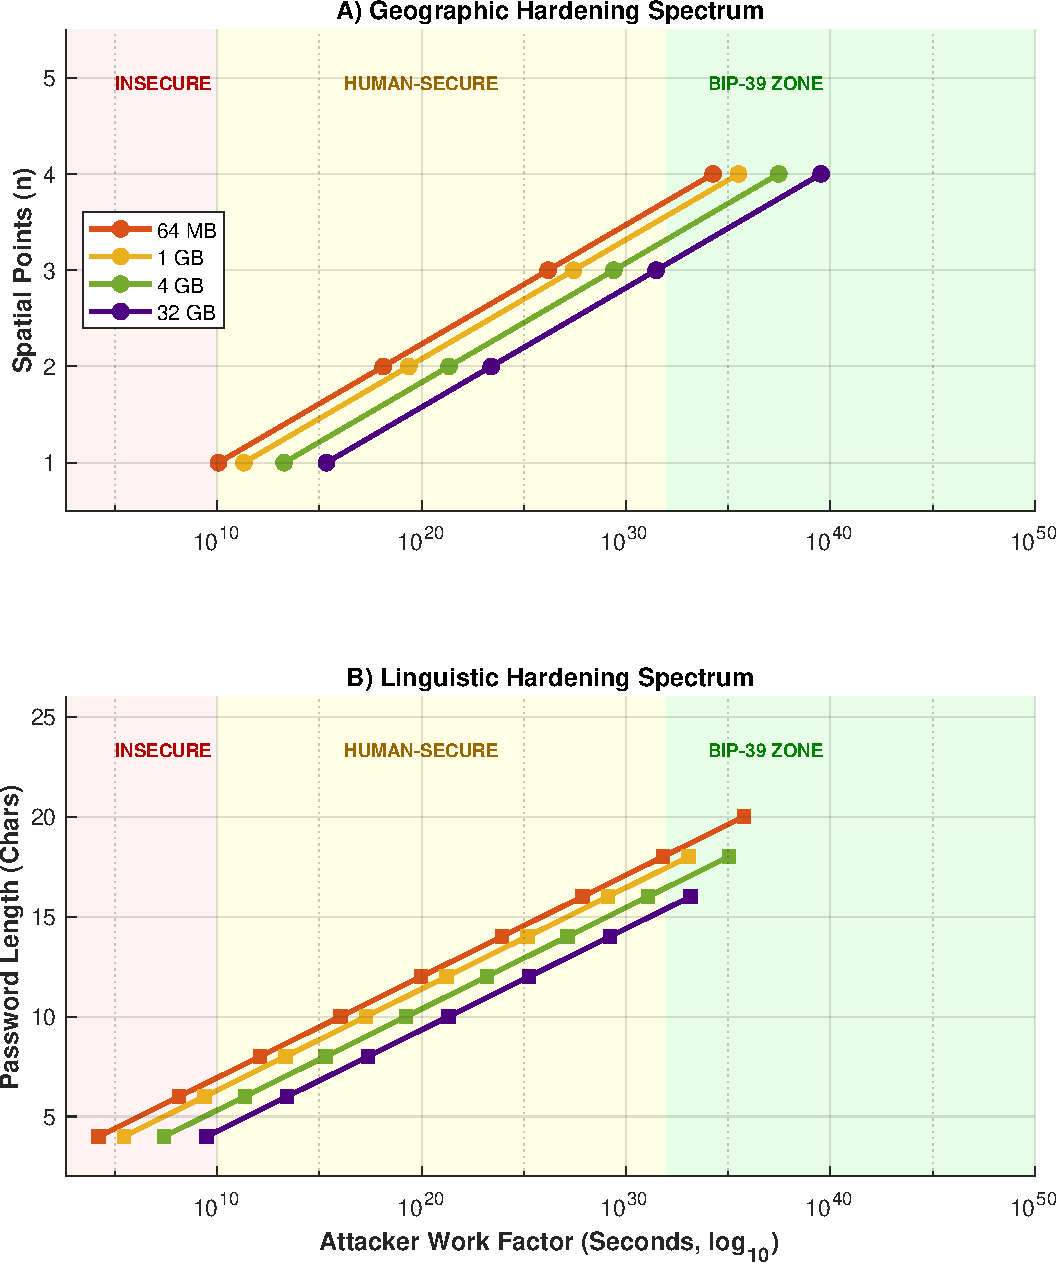
\includegraphics[width=0.9\textwidth]{img/Hardening_Spectrum_No16G.pdf}
    \caption{Attacker-adjusted brute-force resistance under Argon2id hardening. Top: Spatial points $n$ (Y-axis) vs.\ attacker work factor; bottom: password length (Y-axis) vs.\ attacker work factor. Each line is a memory tier $m$; security zones are shaded.}
    % TODO: Update image file img/Hardening_Spectrum_No16G.pdf - subfigure labels should use (A) format instead of A). Also check whether overlapping content in figure affects readability.
    \label{fig:hardening_spectrum}
\end{figure}

Table~\ref{tab:combined_spatial_computational} reports defender-side latency and attacker time-to-compromise for spatial secrets with increasing numbers of points $n$, evaluated across Argon2id memory settings ranging from 64~MiB to 8~GiB. Spatial entropy values for each point count are taken from Table~\ref{tab:raw_radius_entropy}. Defender latency corresponds to CPU-side Argon2id execution, while attacker time-to-compromise reflects single-GPU brute-force attempts under the assumed \mbox{attacker model.}


The reported values show that increasing the number of spatial points rapidly dominates brute-force resistance, such that modest Argon2id memory settings already yield extremely large attacker work factors for $n \ge 3$. At the same time, defender-side latency increases only linearly with the Argon2id memory parameter, remaining below one second for memory settings up to 256~MiB and below five seconds at 2~GiB.

\begin{table}[H]
\setlength{\tabcolsep}{3.96mm}
\caption{Combined brute-force resistance for multi-point spatial secrets under Argon2id hardening. Cell shading indicates security zone (Section~\ref{sec:security_evaluation}).}
\label{tab:combined_spatial_computational}
\begin{tabularx}{\linewidth}{rccccc}
\toprule
\textbf{Memory} & \textbf{Defender} & \multicolumn{4}{c}{\textbf{Time-to-Compromise (s)}} \\
\textbf{(MiB)} & \textbf{Latency (s)} & \textbf{\boldmath{$n=1$}} & \textbf{\boldmath{$n=2$}} & \textbf{\boldmath{$n=3$}} & \textbf{\boldmath{$n=4$}} \\
\noalign{\hrule height 0.5pt}
64   & 0.14 &
\cellcolor{humanscale}$1.1\times10^{10}$ &
\cellcolor{humanscale}$2.3\times10^{24}$ &
\cellcolor{supersecure}$4.1\times10^{37}$ &
\cellcolor{supersecure}$7.5\times10^{50}$ \\

128  & 0.29 &
\cellcolor{humanscale}$2.3\times10^{10}$ &
\cellcolor{humanscale}$4.9\times10^{24}$ &
\cellcolor{supersecure}$8.6\times10^{37}$ &
\cellcolor{supersecure}$1.6\times10^{51}$ \\

256  & 0.62 &
\cellcolor{humanscale}$6.7\times10^{10}$ &
\cellcolor{humanscale}$1.4\times10^{25}$ &
\cellcolor{supersecure}$2.5\times10^{38}$ &
\cellcolor{supersecure}$4.6\times10^{51}$ \\

512  & 1.22 &
\cellcolor{humanscale}$2.5\times10^{11}$ &
\cellcolor{humanscale}$5.3\times10^{25}$ &
\cellcolor{supersecure}$9.6\times10^{38}$ &
\cellcolor{supersecure}$1.8\times10^{52}$ \\

1024 & 2.43 &
\cellcolor{humanscale}$9.9\times10^{11}$ &
\cellcolor{humanscale}$2.1\times10^{26}$ &
\cellcolor{supersecure}$3.8\times10^{39}$ &
\cellcolor{supersecure}$7.1\times10^{52}$ \\

2048 & 4.92 &
\cellcolor{humanscale}$3.9\times10^{12}$ &
\cellcolor{humanscale}$8.3\times10^{26}$ &
\cellcolor{supersecure}$1.5\times10^{40}$ &
\cellcolor{supersecure}$2.8\times10^{53}$ \\

4096 & 10.0 &
\cellcolor{humanscale}$1.6\times10^{13}$ &
\cellcolor{humanscale}$3.4\times10^{27}$ &
\cellcolor{supersecure}$6.0\times10^{40}$ &
\cellcolor{supersecure}$1.1\times10^{54}$ \\

8192 & 20.5 &
\cellcolor{humanscale}$6.5\times10^{13}$ &
\cellcolor{humanscale}$1.4\times10^{28}$ &
\cellcolor{supersecure}$2.4\times10^{41}$ &
\cellcolor{supersecure}$4.4\times10^{54}$ \\

\noalign{\hrule height 0.5pt}
16,384 & 46.9 &
\cellcolor{humanscale}$2.6\times10^{14}$ &
\cellcolor{humanscale}$5.6\times10^{28}$ &
\cellcolor{supersecure}$9.5\times10^{41}$ &
\cellcolor{supersecure}$1.8\times10^{55}$ \\

32,768 & 104.0 &
\cellcolor{humanscale}$1.0\times10^{15}$ &
\cellcolor{humanscale}$2.2\times10^{29}$ &
\cellcolor{supersecure}$3.8\times10^{42}$ &
\cellcolor{supersecure}$7.2\times10^{55}$ \\
\noalign{\hrule height 1.0pt}
\end{tabularx}


\noindent{\footnotesize{\textbf{Shading legend:}
\cellcolor{insecure}Insecure ($<$$10^{10}$ s),
\cellcolor{humanscale} Human-Scale ($10^{10}$--$10^{32}$ s),
\cellcolor{supersecure} Super-Secure/BIP-39 ($\ge$$10^{32}$ s).}}
\end{table}



Relative to the BIP-39 equivalence criterion defined in Section~\ref{sec:security_evaluation} (time-to-compromise exceeding $10^{32}$ s), the table demonstrates that combined spatial and computational hardening achieves cryptographic-strength brute-force resistance without requiring extreme KDF parameters. This illustrates how spatial expansion of the search space reduces reliance on aggressive computational hardening, enabling strong security guarantees while preserving practical usability.

\subsubsection*{Targeted Attacker Scenario} 

{\textls[-25]{The values in Table~\ref{tab:combined_spatial_computational} assume the global nominal spatial entropy ($H_{\text{anchor}} \approx 45.7$ bits}). For a demographically informed attacker who knows the user's city of residence---a scenario supported by findings in~\cite{Sun2012, Thorpe2013, AlAmeen2014}---the anchor entropy collapses to $\approx$$27.4$ bits (Urban dictionary, Table~\ref{tab:entropy_dictionaries}), a reduction of $\approx$$18.3$ bits. For $n=1$, this brings the unaided spatial entropy below any practically secure threshold. However, the Argon2id hardening layer compensates: at $m = 256$~MiB, the attacker time-to-compromise for a single-point secret under the targeted prior is $\approx$$6.7 \times 10^{10} / 2^{18.3} \approx 1.7 \times 10^{5}$~s ($\approx$$2$~days), which falls in the Insecure zone. Increasing to $n = 3$ points restores the combined entropy to $\approx$$108$ bits even under the urban anchor, placing the work factor firmly in the Human-Scale Secure zone at all memory settings $\ge$$64$~MiB. This confirms that multi-point selection is essential for security against targeted adversaries.}



%%%%%%%%%%%%%%%%%%%%%%%%%%%%%%%%%%%%%%%%%%
\section{Discussion\label{sec6}}

%\remove{The results presented in this work show that spatial memory, when combined with modern memory-hard key derivation functions, can meaningfully reshape the traditional security-usability trade-off in cryptographic key management. Rather than attempting to force users to reliably generate or retain abstract high-entropy secrets, GeoVault leverages a cognitive domain in which humans demonstrate strong and durable recall. The empirical and analytical results indicate that spatially anchored secrets exhibit a substantially higher effective entropy floor than human-chosen passwords under realistic offline attacker models, and that this advantage can be amplified through hardware-bound computational hardening.}
{GeoVault rests on a concrete premise: instead of forcing users to memorize abstract symbol sequences, derive keys from places they already know. The results confirm that this shift is quantitatively meaningful. Spatially anchored secrets carry a substantially higher effective entropy floor than human-chosen passwords under the same attacker priors, and Argon2id hardening amplifies this margin non-linearly as memory costs approach GPU VRAM capacity.}

\subsection{Effective Entropy of Spatial Mnemonics}

%\remove{A central finding of this study is that spatial mnemonics provide a higher baseline of effective entropy than linguistic secrets selected by humans.}
{Spatial mnemonics provide a measurably higher baseline of effective entropy than linguistic secrets selected by humans.} As shown in Section~\ref{sec:entropy_floors}, even pessimistic attacker models that restrict guesses to semantically meaningful spatial dictionaries, such as habitable land, coastlines, or urban regions, retain effective entropy levels on the order of $40$--$42$ bits for a single spatial cell. This stands in contrast to human-chosen passwords and passphrases, which empirical studies consistently place well below $20$ effective bits under realistic offline guessing strategies.

However, spatial entropy is not immune to demographic reduction. Research on geographic password systems~\cite{Sun2012, Thorpe2013, AlAmeen2014} documents that a targeted attacker who knows the user's city of residence can restrict the search to an urban-scale dictionary, collapsing the anchor-point entropy from $\approx\!45.7$ bits to $\approx\!27.4$ bits---a reduction of $18.3$ bits. This finding applies to the \emph{anchor point} (the first selected location) and propagates into every subsequent point's contribution: the total $n$-point entropy shifts downward by the same fixed offset regardless of $n$. Critically, this does not eliminate the utility of multi-point selection. As demonstrated in the targeted attacker analysis of Section~\ref{sec:defense_in_depth}, $n=3$ points under the urban prior still reach approximately $108$ bits of combined spatial entropy, placing the work factor firmly in the Human-Scale Secure zone at all evaluated Argon2id settings. The 27.4-bit figure therefore reinforces rather than undermines the paper's core recommendation: a minimum of $n \geq 3$ spatial points is required to maintain adequate security margins against a demographically informed adversary,
 regardless of the computational hardening applied.

%\remove{This higher entropy floor alters the practical boundary of what can be considered usable for human-memorable secrets. While linguistic recall rapidly collapses under selection bias, spatial recall preserves a larger and more evenly distributed search space. The results indicate that a small number of spatial selections, even under conservative attacker assumptions, provide substantially greater resistance to offline attacks than traditional password-based constructions, while remaining compatible with human memory capabilities.}
{This higher entropy floor directly shifts what is practically achievable with human-memorable secrets. Verbal recall collapses under selection bias; spatial recall preserves a larger and more evenly distributed search space. A small number of spatial selections---even under conservative attacker prior assumptions---provides substantially greater offline attack resistance than password-based constructions, with no requirement to memorize abstract symbol strings.}

\subsection{Impact of Memory-Hard Key Derivation}

%\remove{While spatial entropy alone is insufficient to guarantee cryptographic-strength security under all attacker assumptions, the application of memory-hard key derivation functions substantially increases resistance to brute-force attacks. The Argon2id benchmarks reported in Section~\ref{sec:hardware_benchmarks} demonstrate a pronounced asymmetry between defender and attacker capabilities as memory costs increase.}
{Spatial entropy alone does not reach the 128-bit security baseline for single-point configurations under a demographically informed attacker; Argon2id hardening is required to close this gap. The benchmarks in Section~\ref{sec:hardware_benchmarks} reveal a pronounced defender--attacker asymmetry as memory costs increase.} Attacker throughput decreases non-linearly once per-instance memory requirements approach available GPU memory, while remaining feasible, though intentionally costly, for legitimate users operating on commodity CPUs.

This asymmetry arises because Argon2id binds performance to memory bandwidth and capacity rather than raw compute throughput. Under the evaluated attacker model, increasing parallelism does not efficiently compensate for memory exhaustion, resulting in sharp reductions in effective guess rates. %\remove{Consequently, GeoVault converts modest user-side latency into a disproportionate increase in attacker work, allowing spatially anchored secrets to achieve levels of brute-force resistance that approach or exceed established cryptographic security baselines when combined with sufficient effective entropy.}
{Combined, spatial entropy and Argon2id hardening allow GeoVault to reach attacker-adjusted work factors at or above established cryptographic baselines with user-side latencies under 3~s on commodity hardware.}

{Hardware generalizability is quantified in Section~\ref{sec:hardware_benchmarks} (Table~\ref{tab:argon2_defender_cost_consumer}): consumer laptops incur a $1.7\times$--$2.5\times$ latency penalty, placing $m=1024$\,MiB at 2--3\,s. On the attacker side, a four-GPU RTX~4090 cluster raises $\eta$ to $\approx$$264$ at $m=1024$\,MiB---a $\log_2 4 = 2$\,bit reduction in work factor that does not alter the security zone classification for any $n \geq 2$ configuration.}

\subsection{Security Gains from Multi-Point Spatial Selection}

The combination of multiple spatial selections and computational hardening produces rapid growth in attacker-adjusted work factors. As shown in Section~\ref{sec:defense_in_depth}, a small number of spatial points within a realistic dispersion radius, combined with modest Argon2id memory settings, yields work factors that approach or exceed the 128-bit security baseline. These gains come at sub-second to second-scale user-side latency, making the approach practical for interactive use.

Users can trade spatial complexity against computational hardness according to their threat model: more points reduce reliance on extreme KDF parameters, while higher $m$ compensates for fewer points in low-$n$ configurations.

{A useful way to see this flexibility is to ask the following: For each value of $n$, what KDF chaining depth $k$ is needed to reach the Super Secure zone ($\mathcal{W} \geq 10^{32}$\,s), and is the corresponding user-side wait time ($k \times 1.3$\,s) practical? Under the global attacker prior (45.7 bits per point), the answer for $n=1$ is $k \approx 10^{20}$, and for $n=2$, it is $k \approx 5 \times 10^5$ (a wait of roughly 7.5~days)---both completely infeasible. At $n=3$, the search space already exceeds the Super Secure threshold at $k=1$ with a 1.3\,s wait, so no chaining is needed. Under the worst-case urban prior (27.4 bits per point, full demographic leakage of all selected locations), the $n=3$ work factor drops to $\approx\!10^{23}$\,s, which is solidly Human-Scale Secure but below Super Secure; bringing it above the $10^{32}$\,s threshold via chaining alone would require $k \approx 10^9$, again infeasible. However, adding a fourth location keeps the defender burden identical (a single Argon2id invocation over four cell identifiers) and raises the base work factor to $2^{109.6}/53.7 \approx 1.83 \times 10^{31}$\,s. At this point, a chaining depth of only $k=6$ (user-side wait: $6 \times 1.3 \approx 7.8$\,s) crosses the Super Secure threshold: $\mathcal{W}(4, k=6) \approx 1.1 \times 10^{32}$\,s. The practical implication is that users who face the worst-case demographic prior---where a targeted attacker can infer even the secondary and tertiary locations from public data---can compensate with one extra spatial point and a single-digit chaining depth, incurring less than 8\,s of additional wait, without changing any other system parameter.}

\subsection{Threat Model and Limitations}

The security properties of GeoVault are evaluated under a strong offline attacker model in which the adversary has unrestricted access to high-end GPU hardware but no auxiliary side-channel information beyond attacker-prioritized spatial dictionaries. The system does not rely on secrecy of the geospatial encoding scheme or obscurity of the spatial domain. Security derives solely from the effective entropy of user-selected locations and the enforced computational cost of key derivation.

The analysis does not account for targeted social engineering, coercion, or leakage of user-specific spatial preferences. As with all mnemonic-based systems, knowledge of a user's habits, routines, or personal history---inferred from social networks, tagged photographs, or application location data---could reduce the effective search space if spatial choices are overly predictable. {To quantify this risk, consider a worst-case public-information scenario where the attacker recovers the user's home city from a social-media profile, reducing the anchor's effective entropy from the global value of $45.7$\,bits to the urban-scale floor of $H_\text{anchor}\approx 27.4$\,bits (Section~\ref{sec:clustering}). If the attacker further infers---from tagged photographs and check-in history---that all $n$ selected locations lie within the same city, every spatial point collapses to the same urban prior, giving a total entropy of $H_\text{spatial} = n\times 27.4$\,bits. For $n=3$, this yields $82.2$\,bits, which---combined with the Argon2id work factor at $m=1024$\,MiB---maintains an attacker-adjusted work factor above the Human-Scale Secure threshold. Complete demographic leakage across all $n$ points therefore represents the tight lower bound on effective entropy; in practice, secondary and tertiary points are rarely as publicly documented as the anchor, so the true exposure lies between this floor and the uninformed model. The core recommendation of $n\geq 3$ points with $m\geq 1$\,GiB therefore remains sufficient even under full urban leakage of the anchor.} Additionally, this work assumes accurate user recall within the resolution of the spatial encoding scheme. %\remove{While tolerance buffers are incorporated into the entropy analysis, future implementations may benefit from explicit error-correction or fuzzy matching mechanisms to accommodate imperfect recall without expanding the attacker's advantage.}
{The current protocol provides no error tolerance for recall precision: a single-cell recall error (selecting a geographically adjacent 3\,m $\times$ 3\,m tile rather than the originally selected cell) produces a completely different KDF input string, causing 100\% key derivation failure regardless of $n$ or $m$. This is a fundamental usability limitation. Future work should explore error-tolerant extensions---such as a nearest-cell retry window or a spatially defined equivalence class---provided any such relaxation does not increase the attacker's effective dictionary size beyond the security margins established in Section~\ref{sec:defense_in_depth}.}

{A significant limitation of the present work is the absence of an empirical user study. All claims regarding the usability of spatial memory as a cryptographic input---including long-term retention of location-based secrets, recall accuracy under realistic conditions, reduced cognitive load relative to alphanumeric passphrases, and the practical tolerability of the Argon2id computation latency---are inferred from the cognitive psychology and geographic password literature rather than validated through direct experimentation with human participants. While the cited studies~\cite{Montello1998, McNamara2003, Konkle2010, Lukavsky2017, Thorpe2013, MacRae2016} provide strong indirect evidence that spatial memory is more robust and durable than linguistic recall, they were not designed to evaluate the specific GeoVault workflow, and their findings may not transfer directly to the key derivation context. The central claim of the paper---that spatially anchored secrets offer a practical security and usability advantage over linguistic passwords---cannot be fully verified without a controlled user study. Future work should conduct such a study, measuring at minimum (1)~long-term recall accuracy of encoded locations over periods of four or more weeks; (2)~user error rates and the resulting key derivation failure rate; (3)~user-perceived cognitive load compared to BIP-39 mnemonic phrases; and (4)~empirical selection distributions within each spatial dictionary stratum, to calibrate the within-stratum fraction $f_s$ (Equation~\eqref{eq:biased_entropy}) and validate the area-based entropy upper bounds that underlie Section~\ref{sec5}'s security zone classifications. {A dedicated study should further examine accessibility for populations with reduced spatial cognitive ability, including elderly users and individuals with navigation-related impairments, for whom spatial recall may be a less reliable secret~substrate.}}

\subsubsection*{Quantum Adversary Model}

{The threat model evaluated in this paper assumes a classical GPU-based attacker. Under a quantum adversary, Grover's algorithm~\cite{Grover1996} provides an asymptotic $\sqrt{|\mathcal{D}|}$ speedup on unstructured search, which in bit terms, halves the effective entropy of any search space-based secret. Applied to GeoVault, this reduces the per-point spatial entropy from $45.7$\,bits to $\approx$$22.9$\,bits under a quantum attacker with no demographic knowledge, and from $27.4$\,bits to $\approx$$13.7$\,bits under the worst-case urban prior. For $n=3$ points under the uninformed quantum attacker, the total effective entropy is $3 \times 22.9 = 68.7$\,bits; under the urban prior, it is $3 \times 13.7 = 41.1$\,bits. Both values remain above the Human-Scale Secure threshold before any Argon2id hardening is applied. Shor's algorithm~\cite{Shor1994} is irrelevant to this construction: it attacks integer factoring and discrete logarithm problems that underlie asymmetric cryptography, not the symmetric hashing and memory-hard computation performed by Argon2id. Argon2id itself has no known quantum speedup beyond Grover; its memory-hardness argument is independent of the computational model. The practical implication is that GeoVault's $n \geq 3$ recommendation provides a meaningful security margin against a quantum attacker under the uninformed prior, but is insufficient under full urban leakage: an $n=4$ configuration ($4 \times 13.7 = 54.8$\,bits) restores a comfortable margin. A full post-quantum security analysis of memory-hard functions under more refined quantum random-access memory (QRAM) models is an open research problem and is beyond the scope of this work.}

{Physical side-channel attacks---such as timing analysis, power consumption profiling, or memory-access pattern leakage during Argon2id evaluation---are implementation-dependent and fall outside the scope of the protocol-level security model evaluated here. Their relevance and severity depend on the execution environment (browser, mobile app, hardware token) and are left for implementation-level security analysis in future work.}

\subsection{Implications for Human-Centered Key Management}

%\remove{The findings of this study suggest that spatial memory constitutes a viable and underutilized resource for cryptographic key management. By aligning security mechanisms with a cognitive domain in which humans demonstrate strong long-term retention, GeoVault shows that strong offline resistance need not be achieved at the expense of usability. Unlike traditional brainwallets, which rely on abstract linguistic recall and suffer severe entropy collapse, spatially anchored mnemonics provide a higher baseline of effective entropy under realistic attacker models.

%More broadly, GeoVault illustrates how hardware-enforced asymmetry and cognitive ergonomics can be combined to design secure systems that remain usable under real-world constraints. This perspective opens new directions for key management, particularly in scenarios where physical storage of secrets is undesirable or impractical, and where long-term memorability is a primary concern.} 
{Spatial memory is a viable and largely untapped resource for cryptographic key management. Unlike traditional brainwallets, where abstract linguistic recall collapses under selection bias, spatially anchored secrets maintain a substantially higher effective entropy floor under realistic offline attacker models. GeoVault shows that strong offline resistance does not require abstract symbol memorization: three freely selected map points suffice under the evaluated attacker priors.}

{The broader implication is that cognitive ergonomics deserves the same analytical rigor as computational hardness in the design of key management systems. This is especially pertinent where physical key storage is undesirable and long-term memorability is the overriding design constraint.}

%%%%%%%%%%%%%%%%%%%%%%%%%%%%%%%%%%%%%%%%%%
\section{Conclusions\label{sec7}}

%\remove{This work introduced \textit{GeoVault}, a spatially anchored key management framework that leverages human spatial memory in combination with memory-hard cryptographic primitives to address persistent security-usability limitations in mnemonic-based secret storage. By grounding key derivation in spatial locations rather than purely linguistic inputs, GeoVault exploits a cognitive capability that is well-supported by empirical research, while remaining compatible with standard offline cryptographic threat models.}
{\textit{GeoVault} demonstrates that replacing abstract symbol sequences with remembered geographic locations changes the security--usability trade-off in a quantitatively significant way. Users who struggle to reliably store a 12-word BIP-39 phrase can instead anchor a cryptographic key to a small set of familiar places---a spatial recall task that cognitive psychology consistently associates with strong, durable memory retention.}

%\remove{Through information-theoretic analysis, we showed that spatially anchored secrets exhibit a substantially higher effective entropy floor than human-chosen passwords under realistic attacker priors. Empirical benchmarking further demonstrated that when this spatial entropy is combined with a memory-hard key derivation function such as Argon2id, brute-force resistance becomes strongly influenced by hardware constraints. In particular, increasing memory costs toward GPU VRAM limits results in a pronounced, non-linear reduction in attacker throughput, creating a favorable asymmetry between legitimate users and offline adversaries.}
{The entropy model quantifies this advantage directly: a single geographically typical location carries 45.7~bits of effective entropy under the global attacker prior---more than twice the effective entropy of a typical human-chosen password. When $n \geq 2$ locations are combined with Argon2id hardening, brute-force cost grows non-linearly with memory cost by exploiting the VRAM bottleneck of GPU hardware, converting a user-side latency of 1.3~s at $m=1024$~MiB into an attacker workload orders of magnitude larger; $n \geq 3$ points are required to reach the Super Secure zone.}

%\remove{The results indicate that GeoVault can achieve attacker-adjusted work factors that approach or exceed those associated with the 128-bit security baseline of BIP-39 mnemonics. The primary driver is spatial dimensionality: selecting $n \geq 3$ geographic points places the system firmly in the Super Secure zone across all evaluated Argon2id memory tiers, and this holds even under a demographically targeted attacker who restricts the search to an urban spatial dictionary ($H_\text{anchor} \approx 27.4$\,bits). Computational hardening via Argon2id amplifies these margins and provides a tunable usability-security trade-off, but cannot substitute for adequate spatial dimensionality: single-point configurations remain in the Insecure zone under the targeted-attacker prior regardless of memory cost or chaining depth.}
{The key driver is spatial dimensionality. Selecting $n \geq 3$ geographic points places GeoVault firmly in the Super Secure zone ($\mathcal{W} \geq 10^{32}$~s) across all evaluated Argon2id memory tiers under the global attacker prior. Against a demographically targeted attacker with city-level knowledge ($H_\text{anchor} \approx 27.4$~bits per point), $n=3$ achieves Human-Scale Secure resistance ($\mathcal{W} \approx 10^{23}$~s); $n=4$ with a chaining depth of $k=6$ restores the Super Secure zone at an $\approx$8\,s user-side wait. Argon2id amplifies these margins but cannot compensate for insufficient spatial coverage: single-point configurations remain Insecure regardless of memory cost or chaining depth.}

%\remove{Beyond the specific instantiation evaluated in this paper, the GeoVault design highlights a broader principle for key management: aligning cryptographic mechanisms with inherent human cognitive strengths can improve practical security without relying on purely abstract secrets. Future work will explore extensions to three-dimensional and indoor spatial environments, error-tolerant spatial matching mechanisms, multi-user or shared-vault scenarios, and formal analysis under stronger adversarial knowledge assumptions.}
{Open directions include empirical user validation of long-term recall accuracy, error-tolerant matching for approximate location recall, extension to indoor and three-dimensional environments, and shared-vault multi-user protocols. On the formal side, tighter characterization of information leaked by public location traces---social-media check-ins, geotagged photographs---would sharpen the targeted attacker model and clarify the conditions under which urban clustering fully eliminates the security margins \mbox{computed here.}}

%\remove{A key quantitative finding of this work is the \emph{GPU throughput advantage} $\eta(m) = R_\text{GPU}(m)\cdot T_\text{CPU}(m)$ (Equation~\eqref{eq:eta}): at the practical reference tier of $m=1{,}024$\,MiB, the attacker can test roughly 66 candidate secrets for every one key derivation the defender performs. This ratio is independent of KDF chaining depth $k$, which imposes a symmetric cost and therefore cannot improve the attacker-defender balance. The only mechanism that drives $\eta$ toward unity is increasing $m$ beyond GPU VRAM capacity; however, even at 32\,GiB ($\eta\approx 2.5$), the residual advantage is non-negligible. GeoVault's answer is that $\eta$ need not be $\leq 1$: the exponential search-space expansion from spatial dimensionality $n$ provides margins orders of magnitude larger than $\eta$, rendering the residual throughput advantage irrelevant at $n\geq 3$. In summary, GeoVault demonstrates that spatial memory can serve as a viable cryptographic input when combined with hardware-enforced key-derivation cost, provided that the spatial dimensionality is sufficient to absorb the inherent attacker throughput advantage-a principle with broader implications for the design of human-centered key management systems.}
{The GPU throughput advantage $\eta(m) = R_\text{GPU}(m)\cdot T_\text{CPU}(m)$ (Equation~\eqref{eq:eta}) serves as a design decomposition: it isolates the KDF's standalone contribution ($m$-axis) from the search space contribution ($n$-axis), allowing each to be sized independently. At the reference tier, $m=1024$~MiB, $\eta=66$---meaning the search space must contribute at least a factor of 66 in work beyond the KDF cost alone to reach any given threshold, a condition the $n$-axis satisfies exponentially. KDF chaining depth $k$ raises absolute cost symmetrically but leaves $\eta$ unchanged, confirming it acts on the same $m$-axis as memory cost. Only raising $m$ beyond GPU VRAM capacity drives $\eta$ toward unity. The architectural implication is that $\eta$ does not need to reach 1: once spatial dimensionality is sufficient to absorb the residual throughput gap by orders of magnitude, further reductions in $\eta$ via extreme memory cost impose usability penalties without meaningful security gains---a principle applicable to human-centered key management schemes beyond geographic location encoding.}

%%%%%%%%%%%%%%%%%%%%%%%%%%%%%%%%%%%%%%%%%%

\vspace{6pt}
\authorcontributions{Conceptualization,
M.C.; Methodology, M.C.; Software, M.C.; Validation, P.P.; Formal analysis, M.C. and P.P.; Resources, M.C.; Data curation, M.C.; Writing---original draft, M.C.; Writing---review and editing, M.C. and P.P.; Supervision, P.P.; Project administration, M.C. All authors have read and agreed to the published version of the manuscript.}

\funding{Slovenian Research Agency: P2-0270; Ministry of Higher Education, Science and Technology of the Republic of Slovenia: 100-15-0510.}


\dataavailability{The data presented in this study are openly available in [GeoVault Data] at \url{https://github.com/markocorn/geovault-data} (accessed on 12 May 2026),
 reference number [9a5eef3].}
%%%%%%%%%%%%%%%%%%%%%%%%%%%%%%%%%%%%%%%%%%
%% Optional

\conflictsofinterest{The authors declare no conflicts of interest.}

%% Only for journal Encyclopedia
%\entrylink{The Link to this entry published on the encyclopedia platform.}


\begin{adjustwidth}{-\extralength}{0cm}%\centering
\reftitle{References}

\begin{thebibliography}{999}

\bibitem[Adams and Sasse(1999)]{Adams1999}
Adams, A.; Sasse, M.A.
\newblock {Users Are Not The Enemy}.
\newblock {\em Commun.  ACM} {\bf 1999}, {\em 42},~40--46.
\newblock {\url{https://doi.org/10.1145/322796.322806}}.

\bibitem[Bonneau(2012)]{Bonneau2012}
Bonneau, J.
\newblock {The science of guessing: Analyzing an anonymized corpus of 70
  million passwords}.
\newblock In Proceedings of the IEEE Symposium on Security and Privacy, San Francisco, CA, USA, 20--23 May 2012;  pp. 538--552.
\newblock {\url{https://doi.org/10.1109/SP.2012.49}}.

\bibitem[Vasek et~al.(2017)Vasek, Bonneau, Castellucci, Keith, and
  Moore]{Vasek2017}
Vasek, M.; Bonneau, J.; Castellucci, R.; Keith, C.; Moore, T.
\newblock {The bitcoin brain drain: Examining the use and abuse of bitcoin
  brain wallets}.
\newblock In \emph{Financial Cryptography and Data Security}; {Lecture Notes in Computer Science (Including Subseries Lecture
  Notes in Artificial Intelligence and Lecture Notes in Bioinformatics)} (LNSC, volume 9603);
   Springer:  Berlin/Heidelberg, Germany, 2017;  pp.~609--618.
\newblock {\url{https://doi.org/10.1007/978-3-662-54970-4_36}}.

\bibitem[Kuo et~al.(2006)Kuo, Romanosky, and Cranor]{Kuo2006}
Kuo, C.; Romanosky, S.; Cranor, L.F.
\newblock {Human selection of mnemonic phrase-based passwords}.
\newblock In \emph{SOUPS '06: Proceedings of the Second Symposium on Usable Privacy and Security;} {ACM International Conference Proceedings Series}; Association for Computing Machinery: New York, NY, USA, {2006}; Volume 149, pp.~67--78.
\newblock {\url{https://doi.org/10.1145/1143120.1143129}}.

\bibitem[Yang et~al.(2016)Yang, Li, Chowdhury, Xiong, and Proctor]{Yang2016}
Yang, W.; Li, N.; Chowdhury, O.; Xiong, A.; Proctor, R.W.
\newblock {An empirical study of mnemonic sentence-based password generation
  strategies}.
\newblock {In Proceedings of the ACM Conference on Computer and Communications
  Security}, Vienna, Austria, 24--28 October 2016; pp.~1216--1229.
\newblock {\url{https://doi.org/10.1145/2976749.2978346}}.

\bibitem[Pals et~al.(2018)Pals, Tolboom, Suhre, and van Geert]{Pals2018}
Pals, F.F.; Tolboom, J.L.; Suhre, C.J.; van Geert, P.L.
\newblock {Memorisation methods in science education: Tactics to improve the
  teaching and learning practice}.
\newblock {\em Int. J. Sci. Educ.} {\bf 2018}, {\em
  40},~227--241.
\newblock {\url{https://doi.org/10.1080/09500693.2017.1407885}}.

\bibitem[Akaygun and Jones(2014)]{Akaygun2014}
Akaygun, S.; Jones, L.L.
\newblock {Words or Pictures: A comparison of written and pictorial
  explanations of physical and chemical equilibria}.
\newblock {\em Int. J. Sci. Educ.} {\bf 2014}, {\em
  36},~783--807.
\newblock {\url{https://doi.org/10.1080/09500693.2013.828361}}.

\bibitem[Montello(1998)]{Montello1998}
Montello, D.R.
\newblock {A New Framework for Understanding the Acquisition of Spatial
  Knowledge in Large-Scale Environments}. In {\em Spatial and Temporal
  Reasoning in Geographic Information Systems}; Egenhofer, M.J., Golledge,
  R.G., Eds.; Oxford University Press: Oxford, UK,  1998; pp. 143--154.
\newblock {\url{https://doi.org/10.1093/oso/9780195103427.003.0011}}.

\bibitem[McNamara(2003)]{McNamara2003}
McNamara, T.P.
\newblock {How Are the Locations of Objects in the Environment Represented in
  Memory?}
\newblock In \emph{Spatial Cognition III. Spatial Cognition 2002}; Lecture Notes in Artificial Intelligence (Subseries of Lecture
  Notes in Computer Science) (LNAI, volume 2685);  Springer:  Berlin/Heidelberg, Germany,  2003; pp.~174--191.
\newblock {\url{https://doi.org/10.1007/3-540-45004-1_11}}.

\bibitem[McNamara(2012)]{McNamara2012}
McNamara, T.P.
\newblock {Spatial memory: Properties and organization.}
\newblock In {\em Handbook of Spatial Cognition}; American Psychological Association: Washington, DC, USA, 2012; pp. 173--190.
\newblock {\url{https://doi.org/10.1037/13936-010}}.

\bibitem[McNaughton et~al.(1991)McNaughton, Chen, and Markus]{McNaughton1991}
McNaughton, B.L.; Chen, L.L.; Markus, E.J.
\newblock {``Dead reckoning,'' landmark learning, and the sense of direction: A
  neurophysiological and computational hypothesis}.
\newblock {\em J. Cogn. Neurosci.} {\bf 1991}, {\em 3}, 190--202.
\newblock {\url{https://doi.org/10.1162/JOCN.1991.3.2.190}}.

\bibitem[Tari et~al.(2006)Tari, Ozok, and Holden]{Tari2006}
Tari, F.; Ozok, A.A.; Holden, S.H.
\newblock {A comparison of perceived and real shoulder-surfing risks between
  alphanumeric and graphical passwords}.
\newblock In \emph{SOUPS '06: Proceedings of the Second Symposium on Usable Privacy and Security;} {ACM International Conference Proceedings Series}; Association for Computing Machinery: New York, NY, USA, 2006; Volume 149, pp.~56--66.
\newblock {\url{https://doi.org/10.1145/1143120.1143128}}.

\bibitem[Golla et~al.(2017)Golla, Detering, and D{\"u}rmuth]{Golla2017}
Golla, M.; Detering, D.; D{\"u}rmuth, M.
\newblock {EmojiAuth: Quantifying the Security of Emoji-based Authentication}. In Proceedings of the Usable Security Mini Conference (USEC), 
 Santa Clara, CA, USA, 12--14 July 2017.
\newblock {\url{https://doi.org/10.14722/usec.2017.23024}}.

\bibitem[Sun et~al.(2012)Sun, Chen, Fang, and Chang]{Sun2012}
Sun, H.M.; Chen, Y.H.; Fang, C.C.; Chang, S.Y.
\newblock {PassMap: A map based graphical-password authentication system}.
\newblock {In Proceedings of the  ASIACCS 2012---7th ACM Symposium on Information, Computer and
  Communications Security}, Seoul, Republic of Korea, 2--4 May 2012; pp. 99--100.
\newblock {\url{https://doi.org/10.1145/2414456.2414513}}.

\bibitem[Thorpe et~al.(2013)Thorpe, MacRae, and Salehi-Abari]{Thorpe2013}
Thorpe, J.; MacRae, B.; Salehi-Abari, A.
\newblock {Usability and security evaluation of geopass: A geographic
  location-password scheme}.
\newblock {In Proceedings of the  SOUPS 2013---9th Symposium on Usable Privacy
  and Security},  Newcastle, UK, 4--26 July {2013}.
\newblock {\url{https://doi.org/10.1145/2501604.2501618}}.

\bibitem[Biryukov et~al.(2016)Biryukov, Dinu, and Khovratovich]{7467361}
Biryukov, A.; Dinu, D.; Khovratovich, D.
\newblock {Argon2: New generation of memory-hard functions for password hashing
  and other applications}.
\newblock In Proceedings of the 2016 IEEE European Symposium on
  Security and Privacy (EURO S\&P 2016), Saarbrücken, Germany, 21--26 March 2016; pp. 292--302.
\newblock {\url{https://doi.org/10.1109/EuroSP.2016.31}}.

\bibitem[Wetzels(2016)]{Wetzels2016}
Wetzels, J.
\newblock {Open Sesame: The Password Hashing Competition and Argon2}.
\newblock {\em arXiv} {\bf 2016}, arXiv:1602.03097.

\bibitem[Choe et~al.(2019)Choe, Moreshet, Bahar, and Herlihy]{Choe2019}
Choe, J.; Moreshet, T.; Bahar, R.I.; Herlihy, M.
\newblock {Attacking Memory-Hard scrypt with Near-Data-Processing}.
\newblock In \emph{MEMSYS '19: Proceedings of the International Symposium on Memory Systems}; {ACM International Conference Proceedings Series}; Association for Computing Machinery: New York, NY, USA, 2019; pp.
  33--37.
\newblock {\url{https://doi.org/10.1145/3357526.3357570}}.

\bibitem[Das et~al.(2019)Das, Faust, and Loss]{Das2019}
Das, P.; Faust, S.; Loss, J.
\newblock {A formal treatment of deterministic wallets}.
\newblock {In Proceedings of the ACM Conference on Computer and Communications
  Security}, London, UK, 11--15 November 2019;  pp. 651--668.
\newblock {\url{https://doi.org/10.1145/3319535.3354236}}.

\bibitem[Sasse et~al.(2001)Sasse, Brostoff, and Weirich]{Sasse2001}
Sasse, M.A.; Brostoff, S.; Weirich, D.
\newblock {Transforming the `weakest link'---A human/computer interaction
  approach to usable and effective security}.
\newblock {\em BT Technol. J.} {\bf 2001}, {\em 19},~122--131.
\newblock {\url{https://doi.org/10.1023/A:1011902718709}}.

\bibitem[K{\"{a}}vrestad and Nohlberg(2020)]{Kavrestad2020}
K{\"{a}}vrestad, J.; Nohlberg, M.
\newblock {Assisting Users to Create Stronger Passwords Using ContextBased
  MicroTraining}.
\newblock In \emph{ICT Systems Security and Privacy Protection}; {IFIP Advances in Information and Communication Technology} (IFIPAICT, volume 580); Springer: Cham, Switzerland,  2020; pp.~95--108.
\newblock {\url{https://doi.org/10.1007/978-3-030-58201-2_7}}.

\bibitem[{Di Luzio} et~al.(2020){Di Luzio}, Francati, and
  Ateniese]{DiLuzio2020}
{Di Luzio}, A.; Francati, D.; Ateniese, G.
\newblock {Arcula: A secure hierarchical deterministic wallet for multi-asset
  blockchains}.
\newblock In \emph{Cryptology and Network Security
(CANS 2020)}; {Lecture Notes in Computer Science (Including Subseries Lecture
  Notes in Artificial Intelligence and Lecture Notes in Bioinformatics)} (LNSC, volume 12579);  Springer: Cham, Switzerland,  2020; pp.~323--343.
\newblock {\url{https://doi.org/10.1007/978-3-030-65411-5_16}}.

\bibitem[Gutoski and Stebila(2015)]{Gutoski2015}
Gutoski, G.; Stebila, D.
\newblock {Hierarchical deterministic bitcoin wallets that tolerate key
  leakage}.
\newblock In \emph{Financial Cryptography and Data Security
(FC 2015)}; { Lecture Notes in Computer Science (Including Subseries Lecture
  Notes in Artificial Intelligence and Lecture Notes in Bioinformatics)} (LNSC, volume 8975);  Springer:  Berlin/Heidelberg, Germany, 2015; pp.~497--504.
\newblock {\url{https://doi.org/10.1007/978-3-662-47854-7_31}}.

\bibitem[Guri(2018)]{8726762}
Guri, M.
\newblock {Beatcoin: Leaking private keys from air-gapped cryptocurrency
  wallets}.
\newblock In Proceedings of the IEEE 2018 International Congress
  on Cybermatics: 2018 IEEE Conferences on Internet of Things, Green Computing
  and Communications, Cyber, Physical and Social Computing, Smart Data,
  Blockchain, Computer and Information Technology 
  (iThings/GreenCom/CPSCom/SmartData/Blockchain/CIT 2018), Halifax, NS, Canada, 30 July--3 August 2018; pp. 1308--1316.
\newblock {\url{https://doi.org/10.1109/Cybermatics_2018.2018.00227}}.

\bibitem[Yates(2013)]{Yates2013}
Yates, F.A.
\newblock {Selected works: Volume III: Art of memory}.
\newblock In {\em Selected Works: Volume III: Art of Memory}; Taylor and Francis: New York, NY, USA, 2013; Volume 2, pp.~1--400.
\newblock
  {\url{https://doi.org/10.4324/9781315010960/ART-MEMORY-YATES/RIGHTS-AND-PERMISSIONS}}.

\bibitem[Konkle et~al.(2010)Konkle, Brady, Alvarez, and Oliva]{Konkle2010}
Konkle, T.; Brady, T.F.; Alvarez, G.A.; Oliva, A.
\newblock {Scene memory is more detailed than you think: The role of categories
  in visual long-term memory}.
\newblock {\em Psychol. Sci.} {\bf 2010}, {\em 21},~1551--1556.
\newblock {\url{https://doi.org/10.1177/0956797610385359}}.

\bibitem[Lukavsk{\'{y}} and D{\v{e}}cht{\v{e}}renko(2017)]{Lukavsky2017}
Lukavsk{\'{y}}, J.; D{\v{e}}cht{\v{e}}renko, F.
\newblock {Visual properties and memorising scenes: Effects of image-space
  sparseness and uniformity}.
\newblock {\em Atten. Percept. Psychophys.} {\bf 2017}, {\em
  79},~2044--2054.
\newblock {\url{https://doi.org/10.3758/S13414-017-1375-9/FIGURES/4}}.



\bibitem[MacRae et~al.(2016)MacRae, Thorpe, and Salehi-Abari]{MacRae2016}
MacRae, B.; Thorpe, J.; Salehi-Abari, A.
\newblock {GeoPassNotes: Strengthening GeoPass with User Notes for Improved
  Memorability}.
\newblock In Proceedings of the Twelfth Symposium on Usable
  Privacy and Security (SOUPS 2016), Denver, CO, USA, 22--24 June  2016.

\bibitem[Al-Ameen and Wright(2014)]{AlAmeen2014}
Al-Ameen, M.N.; Wright, M.
\newblock {Security and Usability of Geographic Location-Passwords}.
\newblock In Proceedings of the Tenth Symposium on Usable
  Privacy and Security (SOUPS 2014),  Menlo Park, CA, USA, 9--11 July 2014.

\bibitem[Jiang and Stefanakis(2018)]{Jiang2018a}
Jiang, W.; Stefanakis, E.
\newblock {What3Words Geocoding Extensions}.
\newblock {\em J. Geovis. Spat. Anal.} {\bf 2018},
  {\em 2}, 7.
\newblock {\url{https://doi.org/10.1007/s41651-018-0014-x}}.

\bibitem[Lee(2009)]{Lee2009}
Lee, J.
\newblock {GIS-based geocoding methods for area-based addresses and 3D
  addresses in urban areas}.
\newblock {\em Environ. Plan. B Plan. Des.} {\bf 2009},
  {\em 36},~86--106.
\newblock {\url{https://doi.org/10.1068/b31169}}.

\bibitem[Arthur(2023)]{Arthur2023}
Arthur, R.
\newblock {A critical analysis of the What3Words geocoding algorithm}.
\newblock {\em PLoS ONE} {\bf 2023}, {\em 18},~e0292491.
\newblock {\url{https://doi.org/10.1371/journal.pone.0292491}}.

\bibitem[Mai et~al.(2022)Mai, Janowicz, Hu, Gao, Yan, Zhu, Cai, and
  Lao]{Mai2022}
Mai, G.; Janowicz, K.; Hu, Y.; Gao, S.; Yan, B.; Zhu, R.; Cai, L.; Lao, N.
\newblock {A review of location encoding for GeoAI: Methods and applications}.
\newblock {\em Int. J. Geogr. Inf. Sci.} {\bf
  2022}, {\em 36},~639--673.
\newblock {\url{https://doi.org/10.1080/13658816.2021.2004602}}.

\bibitem[Goldberg et~al.(2013)Goldberg, Ballard, Boyd, Mullan, Garfield,
  Rosman, Ferrante, and Semmens]{Goldberg2013}
Goldberg, D.W.; Ballard, M.; Boyd, J.H.; Mullan, N.; Garfield, C.; Rosman, D.;
  Ferrante, A.M.; Semmens, J.B.
\newblock {An evaluation framework for comparing geocoding systems}.
\newblock {\em Int. J. Health Geogr.} {\bf 2013}, {\em
  12}, 50.
\newblock {\url{https://doi.org/10.1186/1476-072X-12-50}}.

\bibitem[Zandbergen(2008)]{Zandbergen2008a}
Zandbergen, P.A.
\newblock {A comparison of address point, parcel and street geocoding
  techniques}.
\newblock {\em Comput. Environ. Urban Syst.} {\bf 2008}, {\em
  32},~214--232.
\newblock {\url{https://doi.org/10.1016/j.compenvurbsys.2007.11.006}}.

\bibitem[Efremova et~al.(2018)Efremova, Endres, Vidas, and
  Melnik]{Efremova2018}
Efremova, J.; Endres, I.; Vidas, I.; Melnik, O.
\newblock {A geo-tagging framework for address extraction from web pages}.
\newblock In \emph{Advances in Data Mining. Applications and Theoretical Aspects
(ICDM 2018)};~{Lecture Notes in Computer Science (Including Subseries Lecture
  Notes in Artificial Intelligence and Lecture Notes in Bioinformatics)} (LNAI, volume 10933); Springer: Cham, Switzerland, 2018; pp.~288--295.
\newblock {\url{https://doi.org/10.1007/978-3-319-95786-9_22}}.

\bibitem[Boneh et~al.(2018)Boneh, Bonneau, B{\"{u}}nz, and Fisch]{Boneh2018}
Boneh, D.; Bonneau, J.; B{\"{u}}nz, B.; Fisch, B.
\newblock {Verifiable delay functions}.
\newblock In \emph{Advances in Cryptology--CRYPTO 2018}; {Lecture Notes in Computer Science (Including Subseries Lecture
  Notes in Artificial Intelligence and Lecture Notes in Bioinformatics)} (LNSC, volume 10991); Springer: Cham, Switzerland, 2018; pp.~757--788.
\newblock {\url{https://doi.org/10.1007/978-3-319-96884-1_25}}.

\bibitem[Wesolowski(2019)]{Wesolowski2019}
Wesolowski, B.
\newblock {Efficient verifiable delay functions}.
\newblock In \emph{Advances in Cryptology--EUROCRYPT 2019}; {Lecture Notes in Computer Science (Including Subseries Lecture
  Notes in Artificial Intelligence and Lecture Notes in Bioinformatics)} (LNSC, volume 11478); Springer: Cham, Switzerland, 2019; pp.~379--407.
\newblock {\url{https://doi.org/10.1007/978-3-030-17659-4_13}}.



\bibitem[Mahmoody et~al.(2011)Mahmoody, Moran, and Vadhan]{Mahmoody2011}
Mahmoody, M.; Moran, T.; Vadhan, S.
\newblock {Time-lock puzzles in the random oracle model}.
\newblock In \emph{Advances in Cryptology–CRYPTO 2011}; {Lecture Notes in Computer Science (Including Subseries Lecture
  Notes in Artificial Intelligence and Lecture Notes in Bioinformatics)} (LNSC, volume 6841); Springer: Berlin/Heidelberg, Germany, 2011; pp.~39--50.
\newblock {\url{https://doi.org/10.1007/978-3-642-22792-9_3}}.



\bibitem[Cohen and Pietrzak(2018)]{Cohen2018}
Cohen, B.; Pietrzak, K.
\newblock {Simple proofs of sequential work}.
\newblock In \emph{Advances in Cryptology--EUROCRYPT 2018}; {Lecture Notes in Computer Science (Including Subseries Lecture
  Notes in Artificial Intelligence and Lecture Notes in Bioinformatics)} (LNSC, volume 10821); Springer: Cham, Switzerland, 2018; pp.~451--467.
\newblock {\url{https://doi.org/10.1007/978-3-319-78375-8_15}}.



\bibitem[Shannon(1948)]{Shannon1948}
Shannon, C.E.
\newblock {A Mathematical Theory of Communication}.
\newblock {\em Bell Syst. Tech. J.} {\bf 1948}, {\em 27},~379--423.
\newblock {\url{https://doi.org/10.1002/j.1538-7305.1948.tb01338.x}}.

\bibitem[Choi et~al.(2024)Choi, Choi, and Seo]{Choi2024}
Choi, H.; Choi, S.J.; Seo, S.C.
\newblock {Parallel Implementation of Lightweight Secure Hash Algorithm on CPU
  and GPU Environments}.
\newblock {\em Electronics} {\bf 2024}, {\em 13},~896.
\newblock {\url{https://doi.org/10.3390/electronics13050896}}.

\bibitem[Qiu et~al.(2016)Qiu, Gong, Guo, Liu, Tang, and Yuan]{Qiu2016}
Qiu, W.; Gong, Z.; Guo, Y.; Liu, B.; Tang, X.; Yuan, Y.
\newblock {GPU-based high performance password recovery technique for hash
  functions}. \emph{J. Inf. Sci. Eng.} \textbf{2016}, \emph{32}, 97--112. 

\bibitem[D{\"{u}}rmuth and Kranz(2015)]{Durmuth2015}
D{\"{u}}rmuth, M.; Kranz, T.
\newblock {On password guessing with GPUs and FPGAs}.
\newblock In \emph{Technology and Practice of Passwords
(PASSWORDS 2014)}; { Lecture Notes in Computer Science (Including Subseries Lecture
  Notes in Artificial Intelligence and Lecture Notes in Bioinformatics)} (LNSC, volume 9393);  Springer: Cham, Switzerland, 2015; pp.~19--38.
\newblock {\url{https://doi.org/10.1007/978-3-319-24192-0_2}}.

\bibitem[Nielsen(1994)]{nielsen1994usability}
Nielsen, J.
\newblock {\em Usability Engineering}; Morgan Kaufmann: San Francisco, CA, USA,  1994.

\bibitem[Bonneau et~al.(2012)Bonneau, Herley, {Van Oorschot}, and
  Stajano]{Bonneau2012a}
Bonneau, J.; Herley, C.; {Van Oorschot}, P.C.; Stajano, F.
\newblock {The quest to replace passwords: A framework for comparative
  evaluation of web authentication schemes}.
\newblock {In Proceedings of the IEEE Symposium on Security and Privacy}, San Francisco, CA, USA, 20--23 May 2012;  pp. 553--567.
\newblock {\url{https://doi.org/10.1109/SP.2012.44}}.

\bibitem[{Food and Agriculture Organization of the United
  Nations}(2014)]{FAO_GLC}
{Food and Agriculture Organization of the United Nations}.
\newblock {Global Land Cover SHARE (GLC-SHARE)}.
\newblock FAO Geonetwork Dataset.  2014.
\newblock Available online: \url{} (accessed on 23 March 2026).
% TODO: Add FAO GLC-SHARE dataset URL here

\bibitem[Venter et~al.(2016)]{Venter2016}
Venter, O.; Sanderson, E.W.; Magrach, A.; Allan, J.R.; Beher, J.; Jones, K.R.; Possingham, H.P.; Laurance, W.F.; Wood, P.; Fekete, B.M.; et al.
\newblock Sixteen years of change in the global terrestrial human footprint.
\newblock {\em Nat. Commun.} {\bf 2016}, {\em 7},~12558.

\bibitem[{JEDEC Solid State Technology Association}(2020)]{JEDEC2020DDR5}
\emph{Standard JESD79-5B}; 
\newblock {Double Data Rate 5 (DDR5) SDRAM Standard: JESD79-5B}.
\newblock JEDEC Solid State Technology Association: Arlington, VA, USA,  2020.

\bibitem[{JEDEC Solid State Technology Association}(2022)]{JEDEC2022LPDDR5x}
\emph{Standard JESD79-5C}; 
\newblock {Low Power Double Data Rate 5X (LPDDR5X) Standard: JESD79-5C}.
\newblock JEDEC Solid State Technology Association: Arlington, VA, USA,  2022.

\bibitem[Grover(1996)]{Grover1996}
Grover, L.K.
\newblock A Fast Quantum Mechanical Algorithm for Database Search.
\newblock In Proceedings of the 28th Annual ACM Symposium on
  Theory of Computing, Philadelphia, PA, USA, 22--24 May 1996; pp. 212--219.
\newblock {\url{https://doi.org/10.1145/237814.237866}}.

\bibitem[Shor(1994)]{Shor1994}
Shor, P.W.
\newblock Algorithms for Quantum Computation: Discrete Logarithms and
  Factoring.
\newblock In Proceedings of the 35th Annual Symposium on
  Foundations of Computer Science, Santa Fe, NM, USA, 20--22 November 1994; pp. 124--134.
\newblock {\url{https://doi.org/10.1109/SFCS.1994.365700}}.

%\bibitem[Bauer and Johnson-Laird(1993)]{Bauer1993}
%Bauer, M.I.; Johnson-Laird, P.N.
%\newblock {How Diagrams Can Improve Reasoning}.
%\newblock {\em Psychological Science} {\bf 1993}, {\em 4},~372--378.
%\newblock {\url{https://doi.org/10.1111/j.1467-9280.1993.tb00584.x}}.
%
%\bibitem[Garden et~al.(2002)Garden, Cornoldi, and Logie]{Garden2002}
%Garden, S.; Cornoldi, C.; Logie, R.H.
%\newblock {Visuo-spatial working memory in navigation}.
%\newblock {\em Applied Cognitive Psychology} {\bf 2002}, {\em 16},~35--50.
%\newblock {\url{https://doi.org/10.1002/acp.746}}.
%
%
%\bibitem[D{\"{o}}ttling et~al.(2020)D{\"{o}}ttling, Garg, Malavolta, and
%  Vasudevan]{Dottling2020}
%D{\"{o}}ttling, N.; Garg, S.; Malavolta, G.; Vasudevan, P.N.
%\newblock {Tight verifiable delay functions}.
%\newblock {\em Lecture Notes in Computer Science (including subseries Lecture
%  Notes in Artificial Intelligence and Lecture Notes in Bioinformatics)} {\bf
%  2020}, {\em 12238 LNCS},~65--84.
%\newblock {\url{https://doi.org/10.1007/978-3-030-57990-6_4}}.
%
%\bibitem[D{\"{o}}ttling et~al.(2019)D{\"{o}}ttling, Lai, and
%  Malavolta]{Dottling2019}
%D{\"{o}}ttling, N.; Lai, R.W.; Malavolta, G.
%\newblock {Incremental proofs of sequential work}.
%\newblock {\em Lecture Notes in Computer Science (including subseries Lecture
%  Notes in Artificial Intelligence and Lecture Notes in Bioinformatics)} {\bf
%  2019}, {\em 11477 LNCS},~292--323.
%\newblock {\url{https://doi.org/10.1007/978-3-030-17656-3_11}}.
%
%
%\bibitem[Cheon et~al.(2008)Cheon, Hopper, Kim, and Osipkov]{Cheon2008}
%Cheon, J.H.; Hopper, N.; Kim, Y.; Osipkov, I.
%\newblock {Provably secure timed-release public key encryption}.
%\newblock {\em ACM Transactions on Information and System Security} {\bf 2008},
%  {\em 11},~4.
%\newblock {\url{https://doi.org/10.1145/1330332.1330336}}.
%
%\bibitem[Cathalo et~al.(2005)Cathalo, Libert, and Quisquater]{Cathalo2005}
%Cathalo, J.; Libert, B.; Quisquater, J.J.
%\newblock {Efficient and non-interactive timed-release encryption}.
%\newblock {\em Lecture Notes in Computer Science (including subseries Lecture
%  Notes in Artificial Intelligence and Lecture Notes in Bioinformatics)} {\bf
%  2005}, {\em 3783 LNCS},~291--303.
%\newblock {\url{https://doi.org/10.1007/11602897_25}}.
%
%\bibitem[Choi and Vaudenay(2020)]{Choi2020}
%Choi, G.; Vaudenay, S.
%\newblock {Timed-Release Encryption with Master Time Bound Key}.
%\newblock {\em Lecture Notes in Computer Science (including subseries Lecture
%  Notes in Artificial Intelligence and Lecture Notes in Bioinformatics)} {\bf
%  2020}, {\em 11897 LNCS},~167--179.
%\newblock {\url{https://doi.org/10.1007/978-3-030-39303-8_13}}.
%
%\bibitem[Abusalah et~al.(2019)Abusalah, Kamath, Klein, Pietrzak, and
%  Walter]{Abusalah2019}
%Abusalah, H.; Kamath, C.; Klein, K.; Pietrzak, K.; Walter, M.
%\newblock {Reversible proofs of sequential work}.
%\newblock {\em Lecture Notes in Computer Science (including subseries Lecture
%  Notes in Artificial Intelligence and Lecture Notes in Bioinformatics)} {\bf
%  2019}, {\em 11477 LNCS},~277--291.
%\newblock {\url{https://doi.org/10.1007/978-3-030-17656-3_10}}.
%
%\bibitem[Nguyen et~al.(2019)Nguyen, Yu, Lebdeh, Taouil, and
%  Hamdioui]{Nguyen2019}
%Nguyen, H.A.D.; Yu, J.; Lebdeh, M.A.; Taouil, M.; Hamdioui, S.
%\newblock {A computation-in-memory accelerator based on resistive devices}.
%\newblock {\em ACM International Conference Proceeding Series} {\bf 2019}, pp.
%  19--32.
%\newblock {\url{https://doi.org/10.1145/3357526.3357554}}.

\end{thebibliography}

%%%%%%%%%%%%%%%%%%%%%%%%%%%%%%%%%%%%%%%%%%
\PublishersNote{}
\end{adjustwidth}
%\isPreprints{}{% This command is only used for ``preprints''.
%} % If the paper is ``preprints'', please uncomment this parenthesis.
\end{document}
